
\documentclass[french,a4paper,12pt]{report}
\usepackage[utf8]{inputenc}
\usepackage[T1]{fontenc}
%\Package paramétrage: marge horizontale à 2,5 cm, et la marge verticale à 1,5 cm.
\usepackage{geometry}
\geometry{hmargin=2cm,vmargin=3cm}
\usepackage{eso-pic}
\usepackage{graphicx}
\usepackage{float}
\usepackage{listings}
\usepackage{color}
\definecolor{dkgreen}{rgb}{0,0.6,0}
\definecolor{gray}{rgb}{0.5,0.5,0.5}
\definecolor{mauve}{rgb}{0.58,0,0.82}
\usepackage{pdfpages}
\usepackage{amsmath}

\lstset{frame=tb,
  language=Java,
  aboveskip=3mm,
  belowskip=3mm,
  showstringspaces=false,
  columns=flexible,
  basicstyle={\small\ttfamily},
  numbers=none,
  numberstyle=\tiny\color{gray},
  keywordstyle=\color{blue},
  commentstyle=\color{dkgreen},
  stringstyle=\color{mauve},
  breaklines=true,
  breakatwhitespace=true,
  tabsize=3
}

%\hfill\hbox to 0pt{\hss
\includegraphics[width=7cm]{UTBM_LOGO.png}\hss}\hfill\null\newline

\begin{document}

\title{	Université de Technologie de Belfort-Montbéliard \\
		{\large \textsc{Génie logiciel, spécialisé dans les systèmes embarqués }} \\
		\vspace{1cm}
		Laboratoire de Physique Nucléaire et des Hautes Énergies \\
		{\large \textsc{Contrôle Haptique et Asservissement de la Mécanique des Pianos de concert }}		
	  }
	  
\date{5 Février 2018 -- 13 Juillet 2018 }
	  
\author{Professeur suiveur : GECHTER Franck  \\
		Tuteur de stage		: LEBBOLO Hervé  \\
		Elève				: ROMET Pierre
		}

\makeatletter
  \begin{titlepage}
  \centering
  \
      {\large \textsc{ }}\\
      \textsc{}\\
      
      \vfill
       {\LARGE \textbf{\@title}} \\
    	\vspace{2em}     
      
    \vspace{1cm}
      {\large{	\@date\\
    \vspace{1cm}
       Stage ST50}}\\
    \vspace{1cm}
        {\large \@author} \\
    \vfill
        
\includegraphics[height=0.13\textheight]{UTBM_LOGO.png}
        \hfill
        
\includegraphics[height=0.09\textheight]{LPNHE_LOGO.png}
  \end{titlepage}
\makeatother

\tableofcontents
\parskip=5pt %to redefine line space of text only, and not for "tableofcontents"


%--------------------------------------------------------------------------------------
%
%	Avant Propos
%
%--------------------------------------------------------------------------------------
\part{Préambule}

  \chapter{Remerciement}
  Tout d'abord, je tiens à remercier l'ensemble de mes collègues pour l'accueil des plus chaleureux, au sein du Laboratoire de Physique Nucléaire et des Hautes Energies, ainsi que pour leur présence tout au long de mon stage, ou aide et conseils n'ont jamais fait défaut.
  
  Je voudrais remercier Monsieur Olivier LEDORTZ, ainsi que David MARTIN pour leur aide concernant l'apprentissage du langage VHDL.
  
  Je souhaite remercier Monsieur Eric PIERRE pour sa présence amicale au quotidien, ainsi que pour le temps passé à me former à la conception et au routage de circuit électronique.
  
  Je remercie Monsieur Julien CORIDIAN pour son soutien, ainsi que les conseils et le temps passé à me former aux bonnes pratiques au sein de l'atelier de fabrication.
  
  Je tiens également à remercier Monsieur Antoine LETESSIER pour ce projet, ainsi que la confiance accordée qui m'a permis de mener ce projet dans les meilleures conditions.
  
  Je remercie tout particulièrement mon maître de stage Monsieur Hervé LEBBOLO, pour son implication dans l'encadrement de mon stage, son soutien, ainsi que pour l'ensemble des connaissances transmises tant sur le plan professionnel que pour le partage autour de la musique.
  
  Enfin, je tiens également à remercier mon enseignant suiveur, Monsieur Franck GECHTER, grâce à qui j'ai pu réaliser un stage de fin d'études me permettant d'allier mon métier à une passion, la musique.
  
 \chapter{Introduction}

Dans le cadre de mes études d'ingénieur au sein de l'Université de Technologie de Belfort-Montbéliard, j'ai effectué un stage de fin d'études en laboratoire, d'une durée de 24 semaines, au sein du laboratoire de Physique Nucléaire et des Hautes Énergies à Paris.

Le laboratoire de Physique Nucléaire et des Hautes Énergies est une unité de recherche de l'institut national de physique nucléaire et de physique des particules, institut du CNRS et des universités Sorbonne Université et Paris Diderot.

Mon stage s'est déroulé au sein du service électronique, sous la tutelle de Monsieur Hervé LEBBOLO.

Lors de ce stage, je fus recruté pour participer au projet "CHAMP"; projet interdisciplinaire, initié par Antoine LETESSIER SELVON, Hervé LEBBOLO, Philippe REPAIN, Laurent BESSIER, Thomas HELIE.

Ce projet interdisciplinaire associe de nombreuses compétences en lutherie artisanale, en technique de préparation de piano, en physique, en électronique rapide et en mécanique de précision.

L'objectif est la réalisation d'un système de motorisation asservie de la mécanique d'un piano à queue afin d'offir de nouvelles couleurs aux préparateurs de pianos, ainsi que de nouvelles voies d'expression musicales aux interprètes tout en gardant intact le toucher traditionnel des mécaniques à répétition.

Le laboratoire étant spécialisé dans le domaine de l'électronique de précision et de l'électronique numérique, travaillant sur des projets tel que LSST (Large Synoptic Survey Telescope - Grand télescope d'étude synoptique), ce stage fut pour moi l'occasion d'évoluer dans un domaine des systèmes embarqués que je maîtrisais peu (de par ma formation), l'électronique analogique et numérique, ce qui m'a permis de découvrir et d'acquérir de nouvelles compétences ainsi que les méthodes de développement qui y sont liées.

Suite à cette introduction, nous allons poursuivre avec la présentation du laboratoire (LPNHE), puis nous conclurons cette première partie par la présentation du projet "CHAMP".


  
	\chapter{Présentation du laboratoire}
  Le LPNHE a été fondé par un groupe de chercheurs et enseignants-chercheurs issus de la division « hautes énergies » de l’institut de Physique Nucléaire (IPN) d’Orsay. En 1970, ces spécialistes des chambres à bulles rejoignent l’université Paris VI, puis l’ensemble devient un laboratoire associé au CNRS. À cette époque, la recherche s’y organise principalement autour d’expériences de chambres à bulles au CERN. Le LPNHE a donc derrière lui une longue histoire de collaboration avec le CERN.
  
  Aujourd’hui encore, même si les expériences et projets dans lesquels est engagé le laboratoire se trouvent maintenant sur les cinq continents, le CERN reste l’endroit privilégié où les chercheurs de physique des particules du laboratoire effectuent leur recherche.
  
  Le laboratoire de Physique Nucléaire et des Hautes Énergies est une unité de recherche de l'institut National de Physique Nucléaire et de Physique des particules, institut du CRNS et des universités Sorbonne Université et Paris Diderot. Il est constitué de 12 groupes de recherche, dont un à l’interface physique/biologie, de 3 services techniques (informatique, électronique, mécanique), et de deux services support étant l'administration et la logistique.
  
  Ces programmes couvrent les enjeux actuels de la physique des particules, des astroparticules, et de la cosmologie.
  On retrouve un groupe constitué de:
  \begin{itemize}
  \item  24 enseignants chercheurs
  \item  27 chercheurs
  \item  44 personnels d'appui à la recherche
  \item  20 Doctorants
  \end{itemize}
  \newpage
  
  \section{Présentation des activités}
  Le laboratoire de physique nucléaire et des hautes énergies (LPNHE) est engagé dans plusieurs grands programmes expérimentaux, poursuivis dans le cadre de collaborations internationales auprès de très grandes infrastructures de recherche du monde entier, tel que des centres d’accélérateurs de particules, ainsi que des observatoires. Ces programmes couvrent les enjeux actuels de la physique des particules, des astroparticules, et de la cosmologie :
  
  On retrouve ainsi des travaux portant sur:  
  \begin{itemize}
  \item L'origine des masses et des familles de particules, recherche du boson de Higgs, unification des interactions fondamentales, recherche de la super-symétrie, dimensions supplémentaires de l’espace-temps : thèmes abordés par les expériences CDF et D0 auprès du Tevatron à Fermilab, et par des expériences auprès du Large Hadron Collider au CERN (ATLAS au LPNHE), et enjeux d’un futur collisionneur e+e- pour lequel le LPNHE est engagé dans le développement de détecteurs en silicium.
  
  \item L’asymétrie matière-antimatière et la physique des saveurs lourdes : ce sont les sujets principaux des expériences BaBar au « SLAC National Laboratory », LHCb au CERN et la future SuperB factory en Italie.
  
  \item Les propriétés des neutrinos : participation à l’expérience Tokaï To Kamiokande (T2K) au Japon.
  
  \item Le contenu énergétique de l’univers, matière noire et énergie noire : le groupe Cosmologie du LPNHE joue un rôle déterminant dans Supernovae Legacy Survey (SNLS) auprès du Canadian French Hawaï Telescope dans Supernovae Factory (SNF) et est engagé dans la préparation des projets futurs Large Synoptic Survey Telescope (LSST) et EUCLID.
  
  \item L'origine des rayons cosmiques de très haute énergie : rayons gamma au TeV pour l’observatoire HESS en Namibie, et rayons cosmiques d’ultra haute énergie (10**18 eV) pour l’observatoire AUGER en Argentine.
  \end{itemize}
  
  Depuis la conception des expériences, en passant par l’étude et la réalisation des instruments de détection, la mise au point des systèmes de détection, d’acquisition et de réduction des données, la calibration et le monitorage des détecteurs pendant les longues périodes de prise de données, l’analyse et l’interprétation physique des mesures, pour enfin aboutir aux publications.
  Ce travail s'étale sur plusieurs années, parfois plus de dix ans, réunissant des équipes et développe des compétences extrêmement diversifiées en physique, électronique, informatique ou mécanique. 
  Les théoriciens du LPNHE représentent une petite composante qui enrichit la vie scientifique du laboratoire, ainsi que de la Fédération de Recherche sur les Interactions Fondamentales (FRIF), dont le laboratoire est membre, ce qui favorise un rapprochement plus fort théoriciens-expérimentateurs.
  
  \newpage
  
  \section{Projet et thématique}
  
		Entre 2015 et 2017, le laboratoire de Physique Nucléaire et des Hautes Energie (LPNHE) a travaillé et continue de développer une vingtaine de projets. Ces projets s'intègrent dans différents domaines d'activité au sein du laboratoire que voici.
  	
  \begin{itemize}
		\item Masses et intéractions fondalentales
		
			- L'expérience Atlas, au LHC (Cern), est l'un des deux détecteurs polyvalents du grand collisionneur de hadrons (LHC). Il étudie des domaines de physique très variés, de la recherche du boson de higgs, aux dimensions supplémentaires de l'espace-temps, en passant par les particules qui pourraient former la matière noire. Il regroupe un large ensemble de projets portant sur la désintégration du boson de Higgs, la physique du quark top, les sections efficaces de jets, de la calibration des électrons et des photons, du R\&D pour la fabrication d'un nouveau trajectographe ainsi que pour un "High Granularity Timing Detector".
			
			- Le projet CALICE, portant sur la recherche et le développement d'un nouveau calorimètre auprès de l'International Linear Collider (ILC). Le projet CALICE (Calorimeter for Linear Collider with Electrons) est un projet développé depuis quelques années pour concevoir des calorimètres de hautes granularités, ils pourront donc mesurer avec une grande précision le flux des particules et permettre de discerner les particules très proches lors du développement des gerbes, afin d'avoir un maximum d'informations sur toutes les désintégrations de particules.			
			
			- Le projet DZero, portant sur la physique du boson de Higgs et du top au Tevatron. Après la mise en évidence de la production de quarks top célibataire et la mesure de Delta Ms, la recherche du boson de Higgs est devenu l'enjeu majeur des expériences Dzero et CDF auprès du collisionneur TeVatron à Fermilab. 
			
		\item Asymétrie matière-antimatière
		
			- L'expérience LHCb (Large Hadron Collider Beauty) portant sur la physique des saveurs lourdes au LHC.
				LHCb explore les légères différences qui existent entre matière et antimatière grâce à l’étude d’un type de particule appelé « quark beauté » ou « quark b ». Au lieu d’utiliser un détecteur fermé au niveau du point de collision, tels que ceux d’ATLAS et de CMS, l’expérience LHCb a recours à plusieurs sous-détecteurs conçus pour observer principalement les particules émises « à petits angles », vers l’avant, dans le sens du faisceau.
			
			- L'expérience "BABAR", est une expérience de physique des particules réalisée au Stanford Linear Accelerator Center. Elle est dédiée à l'étude de la physique des mésons B et de la violation de la symétrie CP dans leur désintégration faible.
			
			- Le projet T2K, "T2K" pour Tokai to Kamioka est un nouvel oscillateur à neutrons. Cette expérience de physique des particules est située au Japon, dans laquelle collaborent de nombreux pays. Il s'agit d'une expérience d'oscillation de neutrinos, mesurant un faisceau de neutrinos muoniques à courte (280 m) et longue distance (295 km). Le but principal de T2K est de mesurer l'oscillation des neutrinos muoniques en neutrinos électroniques afin de mesurer le dernier paramètre de la matrice "Pontecorvo-Maki-Nakagawa-Sakata" permettant d'expliquer l'oscillation de neutrinos prédite par Bruno Pontecorvo en 1957.	
			
			- Le projet COMET, mettant en place des expériences de phénoménologie et la modélisation pour la physique des particules. L’expérience recherche la conversion cohérente sans neutrino d’un muon en électron dans un atome d’aluminium muonique, signal éventuel de physique au-delà du Modèle Standard.
			
			- Le projet SHiP (Search for Hidden Particles) est un projet d’expérience à cible fixe ayant comme projectiles les protons de 400GeV du faisceau du SPS (Super Proton Synchrotron) au CERN. Le détecteur est conçu avec une géométrie favorisant la recherche de particules dites invisibles. Ces dernières sont prédites par bon nombre de modèles théoriques et leur confirmation pourrait élucider certains des grands mystères de la physique actuelle telle que l’origine de la masse des neutrinos, de la matière noire ou encore de l’asymétrie baryonique de l’Univers. Ces modèles postulent l’existence de particules interagissant très faiblement avec celles du Modèle Standard comme par exemple les neutrinos stériles, les particules supersymétriques, les axions, ou encore les photons sombres.
			
		\item Rayonnement Cosmique et Matière Noire
			
			- Le projet AUGER.
			En 1938, Pierre Auger a mis en évidence l'existence de grandes gerbes cosmiques atmosphériques contenant des corpuscules ultra pénétrantes; la technique utilisée était celle des "compteurs en coïncidence". Aujourd'hui l'observatoire Pierre Auger continue de fournir à la communauté scientifique des données précises sur les gerbes atmosphériques les plus énergétiques jusqu'à E-10\^20 eV.
			
			- Le projet H.E.S.S est une expérience d'astronomie gamma dans le désert de Namibie. H.E.S.S est constituée de quatre télescopes atmosphériques à effet Cherenkov possédant chacun un miroir d’environ 12 mètres de diamètre, correspondant à un peu plus de 100 m2 de surface réfléchissante, placés aux quatre coins d’un carré de 120 mètres de côté. Ces télescopes opèrent entre environ 100 GeV et quelques dizaines de TeV. Au centre, un cinquième télescope équipé d’un miroir six fois plus grand en surface est sensible aux rayonnements de plus basse énergie, aux alentours de 20 GeV. 
			
			- L'expérience CTA (Cherenkov Telescope Array) constitue la prochaine génération de réseaux de télescopes à effet Cherenkov atmosphérique qui devrait prendre ses premières données à l’horizon 2022. Il a fait l’objet de la constitution d’une collaboration internationale de plus de 1300 scientifiques répartis dans 210 institutions de 32 pays. Ses objectifs sont de couvrir un domaine en énergie des rayonnements cosmiques détectés de dix GeV à plusieurs centaines de TeV avec une sensibilité accrue de plus d’un ordre de grandeur par rapport aux expériences existantes actuellement (essentiellement HESS, MAGIC et VERITAS).
			
			- L’expérience DAMIC (DArk Matter In CCDs) se propose de détecter le recul induit par la matière noire sur les noyaux de silicium composant les détecteurs à couplage capacitif (les CCD) qui servent habituellement de détecteur de photons en astronomie ou de particules en physique des hautes énergies. Le seuil de détection très bas des CCD (3.5 eV pour former une paire électron-trou) et la masse relativement faible du noyau de silicium permettent de sonder le domaine de masse des WIMP (Weakly Interacting Massive Particles) et d’autres candidats matière noire entre 1 et 20 GeV. Ce domaine en énergie est peu accessible aux grands détecteurs à liquide noble du fait de leur seuil de détection plus élevé.
						
			- Le projet DarkSide pour la recherche de matière noire repose sur l’utilisation d’une Chambre à Projection Temporelle (TPC) à l’Argon liquide en double phase. Un détecteur de 50 kg (DS-50) est actuellement en prise de données au LNGS. Il sera suivi par un détecteur de 20 t, DarkSide-20k.
			
			- Le projet XENON.
			Le détecteur XENON1T, développé par la collaboration XENON pour la recherche directe de matière noire, est l’expérience la plus sensible à l’heure actuelle dans la gamme de masse au-delà d’environ 10 GeV. Il est constitué par une TPC (Time Projection Chamber) remplie de 3.5 tonnes de xénon liquide, située dans le laboratoire souterrain du Gran Sasso, en Italie. Il vise à détecter la faible charge et la petite quantité de lumière qui devraient être émises à la suite de l’interaction d’une particule de matière noire avec un noyau de xénon. La construction de XENON1T a commencé en 2013 et s’est achevée en octobre 2015, suivie par une phase de mise en service et de calibration.
			
		\item Cosmologie et énergie noire
		
			- Le projet Supernovae, consiste en l'observation de supernova dans une gamme de redshift.
			
			- Le projet au sol "LSST", vise à l'observation répétée de l'ensemble du ciel visible, en s'affranchissant d'une partie des effets instrumentaux et atmosphériques. Il est basé sur un télescope au sol de 8.4 mètres de diamètre équipé d'une caméra de 3.2 milliard de pixels. L'ensemble, implanté au Chili, couvrira un champ de 9.6 degrés carrés sur le ciel balayé à la cadence d'un champ toutes les 40 secondes. Chaque champ sera ainsi visité 1000 fois durant les 10 ans de prise de données du programme.
			
			- eBOSS/DESI
			L’objectif principal du groupe est la mesure de l’échelle du pic acoustique des oscillations de baryons (BAO, pour Baryon Acoustic Oscillations), qui constitue un indicateur de distance angulaire et une mesure du taux d’expansion au redshift des sources analysées. On obtient ainsi une précision inégalée à haut redshift. Ce pic se mesure comme un excès de corrélation des traceurs de densité à une distance de séparation précise (en coordonnées co-mobiles).
			
			- Étude de la dynamique des systèmes auto-gravitants
			La motivation principale pour la recherche théorique du groupe est le problème de la formation des grandes structures de l’univers. Le défi large est de rendre compte systématiquement des observations pertinentes (distribution des galaxies, lentillage faible, CMB etc.) dans le cadre de la cosmologie standard (« Lambda CDM ») ou de ses variantes, et notamment dans le régime « non-linéaire ». L’accent de la recherche du groupe porte sur des questions fondamentales théoriques dans ce contexte, et il s’attache notamment à comprendre la dynamique non-linéaire de la matière purement gravitante et non-relativiste, approximation valable pour une grande partie de l’évolution de l’univers dans le modèle standard.		
		  	
  \end{itemize}
  
    
%--------------------------------------------------------------------------------------
%
%	Présentation du projet "CHAMP"
%
%--------------------------------------------------------------------------------------
\part{Qu'est ce que le projet "CHAMP" ?}
  \chapter{Présentation}
  
  Ce projet est né de la rencontre de Laurent BESSIÈRES, préparateur de piano intervenant pour les concerts et récitals de la Philarmonique de Paris et de Antoine LETESSIER SELVON, physicien des hautes énergies, directeur de recherche au CNRS et pianiste amateur. 
  
  De leur discution est né un projet au travers duquel ils cherchent à élargir les possibilités de l'instrument en modifiant de manière originale sa mécanique. C'est en s'appuyant sur des techniques modernes qu'ils souhaitent proposer de nouveaux moyens d'expression aux artistes, tout en respectant le lien étroit qu'ils entretiennent avec leur instrument notamment au travers du touché.
  
  \section{État de l'art}
  
  C’est en 1700 que Bartolomeo Cristofori invente la mécanique à échappement et construit le premier instrument à cordes frappées : le piano-forte. Ce sont les balbutiements de l’histoire du piano à queue. Le piano-forte révolutionne la technique pianistique, car il permet à l’interprète de passer par le jeu des doigts, d’une nuance piano à une nuance forte, ouvrant de nouvelles voies à l’expression musicale et à la créativité des compositeurs. Cent vingt-trois ans plus tard, en 1821, Sébastien Érard ajouta un système de répétition à la mécanique de Cristofori et invente la mécanique moderne dite (improprement) à double échappement.

A la même époque, deux progrès techniques et industriels vont donner naissance au piano moderne. D’une part l’utilisation d’acier fondu pour les cordes et d’autre part l’introduction de cadres métalliques en fonte. Par ailleurs, de nombreux brevets seront déposés concernant la table d’harmonie, le croisement des cordes, le chevalet, l’assemblage de la mécanique, etc. 

De telle sorte que, peu avant 1890, l’essentiel de ce qui fait un piano moderne est accompli. À partir de cette date et à la suite d’une concentration industrielle de plus en plus forte, la nécessité de produire le plus d’instruments possibles au moindre coût pour garantir plus de parts de marchés, les innovations vont essentiellement cesser et conduire en moins d’un siècle à la disparition de presque tous les facteurs artisanaux et à l’uniformisation quasi totale des instruments avec pour référence le piano de concert Steinway dont le modèle produit en 1877 réunissait déjà les inventions les plus importantes du XIXe siècle.

\newpage
On peut légitimement se demander quelles sont les lacunes du Steinway d’aujourd’hui, joué par 95\% des pianistes de la planète, qui justifieraient de bouleverser l’état actuel.
De fait, nous ne souhaitons pas nous appuyer sur d’éventuelles lacunes du Steinway ou d’ailleurs de tout autre piano, nous voulons avant tout ouvrir de nouvelles pistes. 
 Ceci en introduisant une source extérieure d’énergie, totalement et délicatement pilotée par l’instrumentiste, nous allons libérer des contraintes auquelles les pianos modernes, les Steinway en particulier, ont répondu de manière optimale, mais qu’ils ont malgré tout intégré.
 
 \section{Motivations}
 
 La mécanique à répétition de Sébastien Érard, brevetée à Londres par son neveu Pierre en 1921, est toujours utilisée aujourd’hui. Pourtant, la demande contemporaine de piano de concerts d’une puissance toujours plus grande (sans perte de sensibilité) n’a jamais été aussi forte. Par ailleurs, au cours des 30 dernières années, des facteurs indépendants ont introduit des innovations (nouveaux alliages pour les cordes, nouvelle structure pour le cadre et la table d’harmonie, etc.) et repensé certains des choix techniques de la fin du XIXe siècle (croisement des cordes, barrage, ...). Ainsi en France, Stephen Paulello, le dernier facteur français de pianos de concert en activité, vient de produire le premier exemplaire de sa dernière création : l’Opus 102. Ce piano de concert fait 3m de long et possède une tessiture de 102 notes (contre environ 2m80 et 88 notes pour les pianos de concert standard). Il comporte de nombreuses innovations et a été accueilli par la critique comme la “Bugatti Royale” des pianos.

La mécanique, de son coté, a peu évolué. L’utilisation de matériaux composites ou la modification de certaines pièces a parfois permis d’explorer quelques pistes (légèreté, coût, endurance, reproductivité) mais de manière limitée car le compromis actuel semble optimal compte tenu des contraintes imposées par la morphologie de l’instrument et de l’énergie qu’un artiste peut raisonnablement fournir pour l’actionner. Compte tenu de ces contraintes, l’ouverture vers de nouvelles expressions sonores par le biais de la mécanique ne semble pas avoir été explorée. Certains développements ont consisté à introduire des éléments passifs, aimants, ressorts, élastiques, à l’intérieur de la mécanique ou sous les touches, mais aucun n’a semblé apporter suffisamment pour emporter l’adhésion des techniciens et surtout des artistes.\newline

	\begin{figure}[!ht]
    \center
    %\hfill\hbox to 0pt{\hss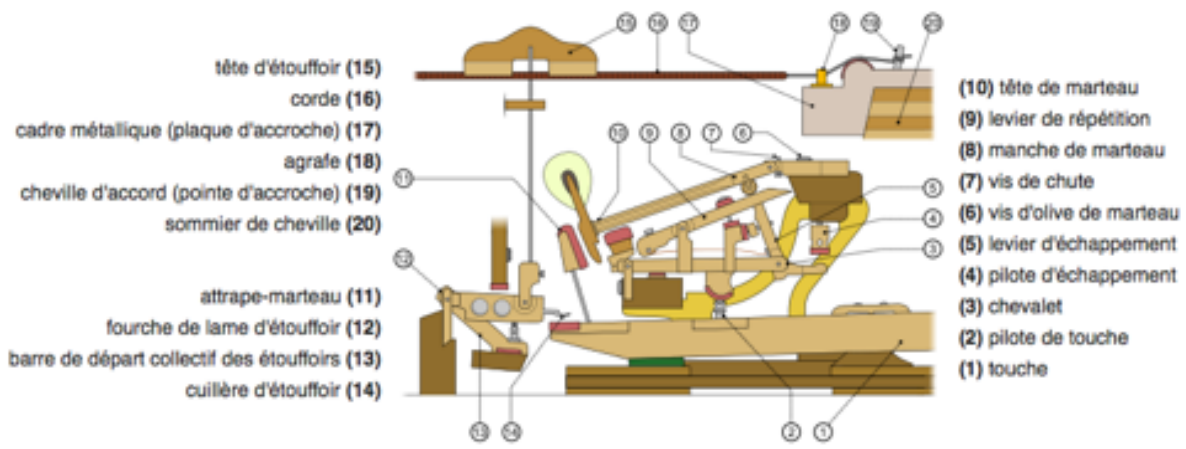
\includegraphics[width=15cm]{MECA_PIANO.png}\hss}\hfill\null
    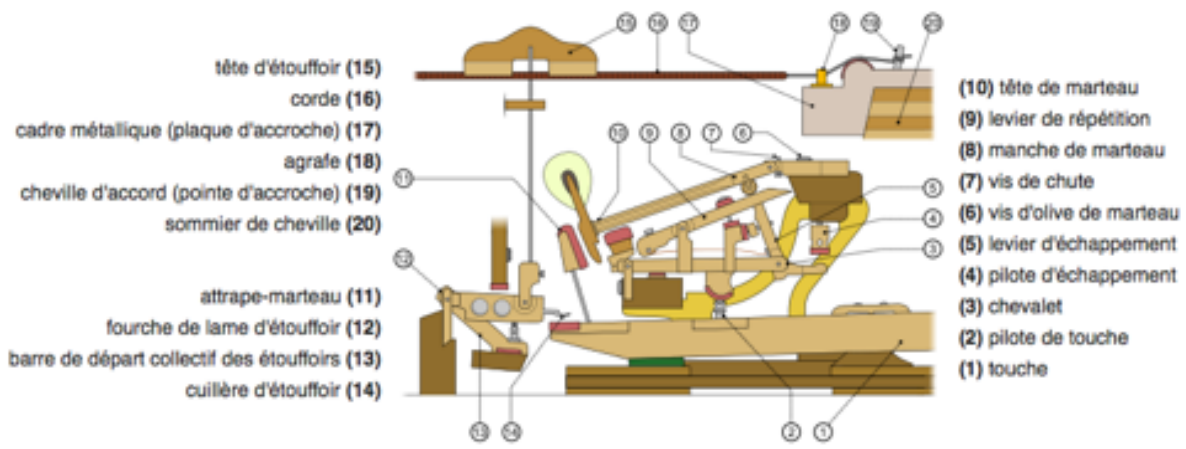
\includegraphics[width=15cm]{MECA_PIANO.png}
    \caption{Schéma de mécanique de Piano}
	\end{figure} 

Côté éléments actifs, l’essentiel des innovations concerne la reproduction autonome par l’instrument d’une musique jouée précédemment (sur lui même ou sur un instrument similaire), c’est le cas par exemple de la technologie "DisklavierTM" mise au point par Yamaha. Il n’y a pas d’interaction directe entre l’artiste et la mécanique augmentée. La mécanique de ces pianos enregistre le jeu de l’artiste puis le restitue sans son aide, avec une perte de sensibilité notable. Il n’y a donc pas d’exploration de nouvelles capacités sonores ou d’augmentation de la palette de couleur de l’instrument, bien au contraire. Notons cependant les explorations de certains chercheurs, comme par exemple Andrew McPherson6 et son “Magnetic Resonator Piano” où des électroaimants placés au-dessus des cordes les maintiennent en résonance sous le contrôle de l’interprète offrant ici très clairement de nouvelles options d’expression.

D’un autre côté, les salles de concerts sont de plus en plus grandes et demandent, malgré une acoustique souvent exceptionnelle, des instruments de plus en plus puissants. Notons également que les orchestres sont aussi plus larges et que les instruments eux-mêmes, des cordes aux cuivres, ont également gagné en puissance. Ainsi on trouve aujourd’hui des pianos de plus de 3m (Fazioli 3,08m) permettant en principe d’obtenir une puissance extrême mais c’est toujours la mécanique de Sébastien Érard qui est employée pour produire le son, une mécanique à la puissance limitée par celle que l’artiste peut lui fournir.

La puissance n’est cependant que l’un des paramètres sur lequel l’addition d’une source extérieure d’énergie permet d’intervenir. À puissance fixe, on peut explorer une répartition différente de l’énergie cinétique entre la masse du marteau et sa vitesse. Cette exploration est très limitée dans le cas d’une mécanique traditionnelle car l’inertie de l’ensemble doit être contenue afin que l’effort d’enfoncement des touches reste tolérable pour l’artiste, surtout à haute vélocité. Il en ressort que les masses des marteaux et le point de frappe, deux éléments qui ont une importance considérable dans la couleur du son, indépendamment de la dynamique, sont aujourd’hui fixés à des valeurs de référence choisies et considérées comme optimales par le fabricant dominant le marché actuel et pour l’essentiel copiées par tous les autres. Insistons néanmoins sur le fait que compte tenu des contraintes décrites ci-dessus (inertie, poids, morphologie), les variations sur ces paramètres sont très limitées, et c’est pourquoi nous nous proposons de lever une partie au moins de ces contraintes.

Ce constat est aussi celui que fait Laurent Bessières qui, après avoir exercé son métier d’accordeur préparateur concert pendant plus de 15 ans auprès des plus grands artistes et dans les plus grandes salles de concert de Paris, aimerait pouvoir offrir d’avantage à ceux qui le souhaitent. Les artistes ont en effet des exigences quant au toucher et à la sonorité souvent contradictoires compte tenu de ce qui peut être fait sur une mécanique ordinaire. Une plus grande latitude dans le mode de transfert d’énergie de la touche au marteau et du marteau à la corde permettrait une exploration d’une palette de couleurs beaucoup plus large et également une meilleure exploitation des nouvelles technologies de cadres et de cordes.

\section{Concepts} 

La mécanique des pianos à queue (figure 1) est constituée de trois pièces principales : la touche, le chevalet et le marteau. Lorsque la touche est enfoncée, elle transmet l’énergie du doigt qui l’enfonce au chevalet qui démultiplie la vitesse d’enfoncement afin de propulser à grande vitesse (jusqu’à plusieurs m/s) le marteau sur les cordes. Les réglages de la mécanique permettent de modifier la sensation de toucher et la production sonore. Ainsi, on peut obtenir un clavier plus léger ou plus lourd et un son plus puissant, plus doux, plus clair ou plus feutré.

Le transfert d’énergie des marteaux aux cordes passe par une impulsion mécanique dont l’amplitude dépend de l’énergie cinétique du marteau (l’énergie cinétique est proportionnelle au produit de la masse du marteau par le carré de sa vitesse) et dont la durée (à vitesse de marteau fixée) dépend de la dureté des feutres, du point de frappe et de l’élasticité des cordes. Les mécaniques standards imposant la masse des marteaux et le point de frappe, le préparateur ne peut jouer pour l’harmonisation que sur les feutres tandis que l’énergie maximale transmise est, toutes choses égales par ailleurs, fixée par la masse du marteau lui-même.

De nombreux articles, rédigés par des spécialistes, concluent (sur la base de leurs expériences) que le poids des marteaux est un élément essentiel de l‘harmonie du piano :

\begin{itemize}
	\item  “Le poids du marteau n'a pas seulement une grande incidence sur le toucher, il en a aussi une sur le son. En ce sens, nous devons bien inclure l'effet sonore du poids du marteau dans toute discussion au sujet du réglage du toucher”; c.f. Boddin Piano Service.

	\item  “[...] appréciation critique d'un piano à queue Steinway modèle S: les marteaux étaient légers, le son semblait irréprochable. Franz accrocha des poids de quelques grammes sur quelques manches de marteau et déplaça ainsi le dit poids dans la "high zone” [région désignant les pianos dits lourds, NDLR]. A l'écoute du son ainsi modifié, leur surprise fut très grande: ça n'était plus seulement du son, on pouvait carrément sentir le son occuper l'espace. La différence fut si importante que Wim s'exclama : "Mais alors, c'est quoi l'intonation !?" Ces mots nous interpellèrent tous. Voilà qui prouve que nous avons bien à réexaminer en profondeur l'idée et la pratique de l'intonation en y intégrant le rôle que joue le poids du marteau, [...]”.

	\item  “D'une façon générale, la majorité des améliorations successives ont toutes cherché à obtenir un son à la fois fort et tenu. La sonorité des pianos actuels donne l'illusion d'une continuité sonore que les facteurs ont toujours cherché à obtenir. A l'inverse, un système élaboré d'étouffoirs permet d'obtenir des sons extrêmement brefs, ce qui fut longtemps impossible. Pour obtenir cette double qualité, la dimension et le poids des marteaux, qui viennent frapper les cordes, se révèlent décisifs. [...] Le rapport de la masse de la corde à la masse du marteau se révèle ici le facteur déterminant” par René Caussé dans Résonance no 5, septembre 1993 Copyright © IRCAM.

\end{itemize}

Le poids d’enfoncement d’une touche de clavier est compris entre 45g et 60g, celui des marteaux est d’un peu moins de 12g dans les basses à moins de 5g dans les aigus, et ce depuis 200 ans. C’est le confort de jeu des pianistes qui l’impose. Pour maintenir l’inertie des touches à un niveau acceptable, il faut également que l’ensemble du poids mis en mouvement ne soit pas trop élevé et donc que le contre-poids (en plomb) mis dans les touches reste faible. Ces deux principes limitent la masse du marteau qui est le seul élément qui pourrait, si on augmentait sa masse, transmettre toute l’énergie qu’un piano de 3m (et plus!) peut développer.



\chapter{Les premières approches}

  \section{Mécanique et Electronique}
Nos premières réflexions sur la réalisation d’un système d’assistance et d’asservissement d’une mécanique de piano à queue démontrent qu’il faut faire appel à des technologies de pointe. Ce qui explique l’aspect novateur de notre projet. Par exemple, les contraintes mécaniques sur les moteurs susceptibles de seconder les doigts dans leur action sont nombreuses. Pour ne citer que les plus essentielles :\newline

	\begin{figure}[!ht]
    \center
    %\hfill\hbox to 0pt{\hss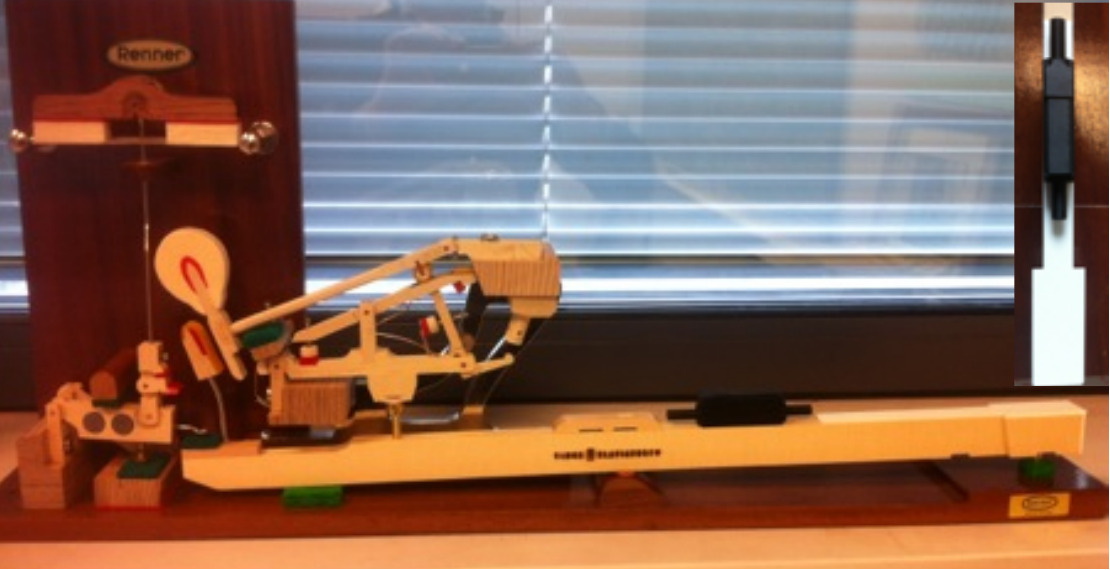
\includegraphics[width=13cm]{MECA_PIANO2.png}\hss}\hfill\null
    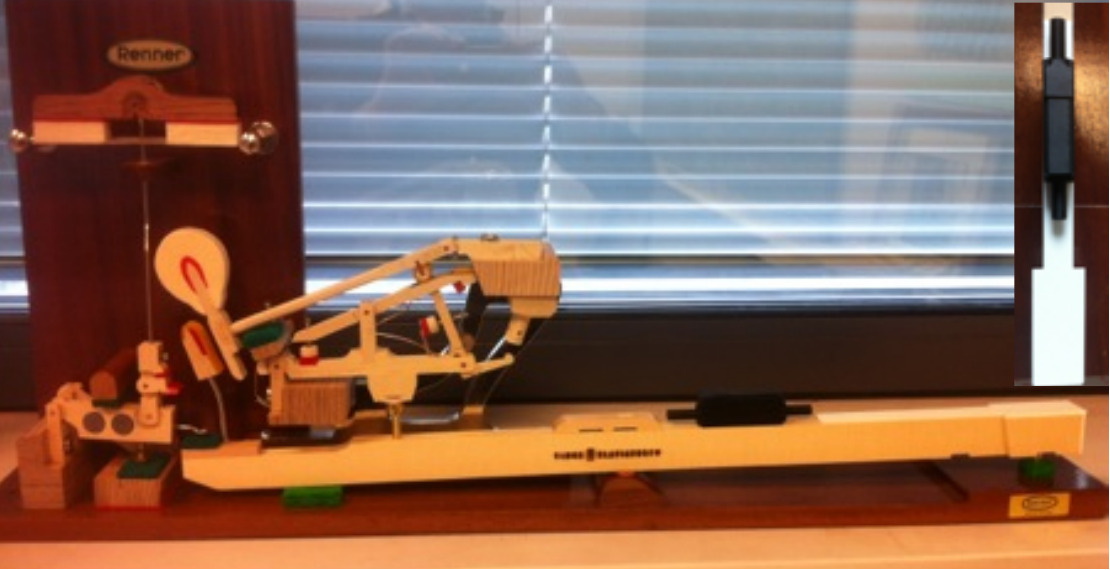
\includegraphics[width=10cm]{MECA_PIANO2.png}
    \caption{Mécanique de Piano}
	\end{figure} 

%Une mécanique de type Renner avec un modèle 3D de l’actuateur linéaire
%envisagé (en noir posé sur la touche) pour donner l’échelle. L’actuateur peut être soit intégré
%dans le sommier en tête de la mécanique sous la cuillère d’étouffoir ou bien positionné à
%l’arrière de celle-ci sur le sommier de cheville. Plusieurs positions seront étudiées. En insert
%une vue de l’actuateur sur la touche qui montre que sa largeur est parfaitement adaptée.

\begin{itemize}
	\item  rapidité : temps de réponse à la milliseconde, vitesse maximum de l’ordre du mètre par
	seconde, accélération de l’ordre de 10 ou 20 g (100 à 200 m/s2 ).

	\item Puissance : force en impulsion de l'ordre de 1kg ou 10N.

	\item encombrement faible: dimension de l'ordre de 1 cm(l) x 1 cm(p) x 5 cm(h).

	\item bruit, inexistant ou négligeable : 10-15 dB à moins de 1m.

	\item précision : positionnement du manche de marteau au dixième (0.1 mm).

	\item fiabilité : durée de vie de milliers d'heures et plus de 10 millions de mouvements.
\end{itemize}

Des moteurs avec ces caractéristiques sont disponibles aujourd’hui et font appel (entre autres) à de puissants aimants miniatures pour les mouvements et à des sondes à effet Hall intégrées pour le positionnement. La figure 5.2 montre un profil de mécanique (c’est à dire la mécanique complète d’une touche individuelle) de la marque Renner, d’autres modèles existent, notamment sur les Steinway, mais leurs caractéristiques essentielles sont semblables. Sur cette même figure, un modèle en impression 3D d’un moteur linéaire de la marque Faulhaber, aux performances mécaniques adaptées à notre problème, est posé sur la touche. On peut voir que ces dimensions sont idéalement adaptées à celles d’un clavier de piano.

L’électronique qui permet la mesure du déplacement des touches (connectée à un capteur de position et/ou un accéléromètre) et qui contrôle l’asservissement doit elle aussi être rapide et précise, si possible intégrée, fiable, puissante et programmable et fera donc appel à de la micro électronique compatible HT (100V) ainsi qu’à des FPGA pour la programmation de l’asservissement et le contrôle du toucher. L’expertise du LPNHE en électronique de pointe et mécanique de précision est un atout déterminant de cette réalisation.

	\begin{figure}[!ht]
    \center
    %\hfill\hbox to 0pt{\hss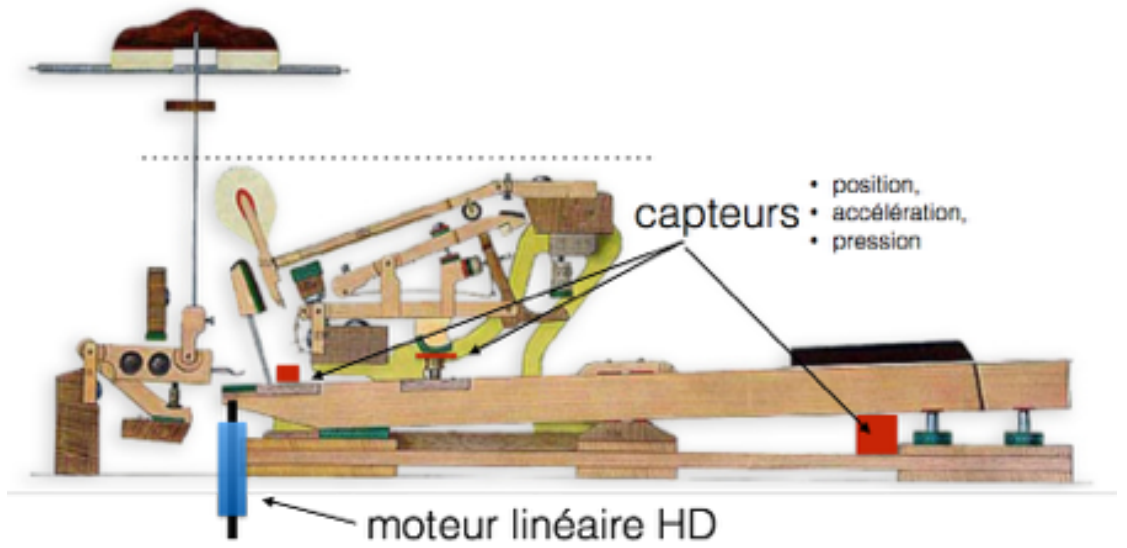
\includegraphics[width=15cm]{MECA_PIANO3.png}\hss}\hfill\null
   	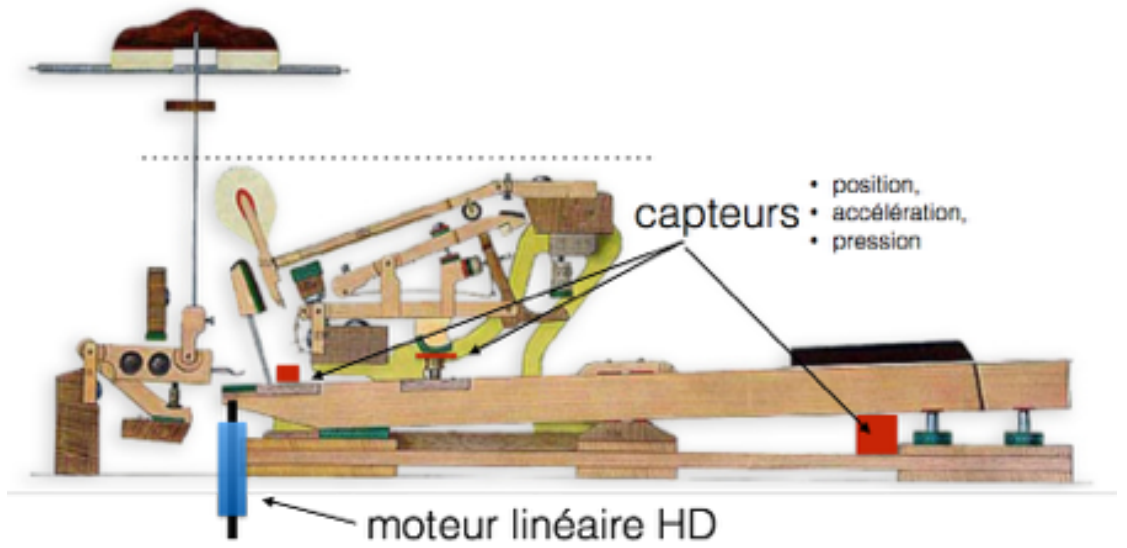
\includegraphics[width=15cm]{MECA_PIANO3.png}
 		\caption{Mécanique de type Renner avec un modèle 3D de l’actuateur linéaire}
	\end{figure}

Pour guider les idées, un schéma envisageable d’implémentation est proposé sur la figure 3. L’implémentation optimale nécessite bien sûr une étude plus approfondie, il s’agit simplement ici de se de fixer les idées. Le moteur et les capteurs de positions sont représentés par les rectangles bleus ou rouges. Sur cette proposition, le rapport (R) entre l’action du moteur et celui du marteau est le même que pour le doigt de l’artiste soit environ 5,5. Les modifications apportées à la mécanique originale sont minimales. Avec un réglage approprié, la sensation de toucher sera adaptable aux désirs de l’artiste et restera très proche des sensations offertes par la mécanique à répétition et ce même si les marteaux sont lourds car le moteur accompagne en le soutenant le mouvement de la touche mais ne s’y substitue pas totalement.

  \section{Boucle d'asservissement}

La qualité de la boucle de feedback est un point essentiel de notre entreprise. C’est ici que l’expertise de Laurent Bessières donne tout son sens musical au projet. L’asservissement devra d’une part donner aux artistes un confort de jeu digne des meilleures mécaniques avec en plus un équilibrage parfait sur toute l’étendue du clavier. D’autre part, et c’est peut être le plus important, un certain nombre de paramètres de la boucle d’asservissement seront modifiables.

L’échappement et la façon dont il se déroule constituent l’épicentre de l’expressivité. Nous en avons bien conscience et notre intention est bien de le conserver tel quel afin que l’artiste ne soit pas perturbé et puisse donner le meilleur de lui même. Le résultat final dépend également d’un mariage harmonieux entre la mécanique/clavier et l’ensemble harmonique et nous devrons procéder par étape. D’abord assurer que l’apport d’énergie peut se faire de manière quasi transparente pour l’artiste, ensuite exploiter les possibilités offertes par cet apport. Deux axes seront explorés en priorité :

\begin{itemize}
\item  le paramétrage de la courbe de réponse de la mécanique en fonction de l’énergie fournie par l’artiste. On peut élargir ou rétrécir la gamme dynamique et rendre la courbe de réponse non linéaire et des degrés aussi divers qu'imaginables.

\item  la modification physique des éléments de la mécanique, comme le poids et les têtes de marteaux et, en allant plus loin, le point de frappe.
\end{itemize}

Sur tous ces domaines, l’expertise de Laurent Bessières est fondamentale aussi bien pour identifier les paramètres de contrôle que pour qualifier leur gamme et pour la bonne intégration de l’ensemble dans l’instrument. La programmation des fonctionnalités dans le FPGA qui calculera les commandes du moteur à partir des données des capteurs sera elle réalisée par les ingénieurs du LPNHE.

\newpage

  \section{Modélisation}

Thomas Hélie, chercheur à l’IRCAM au Laboratoire des Sciences et Technologies de la Musique et du Son, est spécialiste de la modélisation physique d’instruments de musique. L’un de ses projets de recherche concerne notamment la modélisation, l’asservissement et la commande d’une bouche artificielle robotisée, pour le jeux de cuivre. Dans le cadre de notre projet, son expertise nous permettra de modéliser les performances de la boucle de feedback en fonction des paramètres mécaniques que nous pouvons ajuster (position de l’actuateur, nombre, nature et position des capteurs). Disposer d’un modèle nous permettra de choisir les configurations les plus prometteuses avant de les réaliser plutôt que d’avoir à toutes les construire et toutes les essayer.

La méthode des systèmes Hamiltionien à ports (Port Hamiltonian System ou PHS) nous permettra de réaliser ces modèles. Cette approche où le système physique étudié est représenté par un ensemble de composants (éléments stockant de l’énergie, éléments dissipatifs, sources externes) reliés par des connexions conservatives (bilan d’énergie ou de puissance) permet une modélisation numérique relativement simple des systèmes complexes. Cette représentation garantit par ailleurs que les lois de conservations sont satisfaites à toutes les interfaces. La modularité du PHS permet d’envisager une complexité graduelle de la modélisation jusqu’à représenter de manière très réaliste l’ensemble touche, chevalet, marteaux ainsi que les commandes d’étouffoir et les ressorts de rappel. Dans ce cadre, nous nous appuierons également sur les travaux de Xavier Boutillon concernant la modélisation extrêmement réaliste du toucher des mécaniques de piano à queue.

Notons également que l’approche PHS permet d’étudier les réponses non linéaires aux actions extérieures et de calculer les (pré-)contraintes à appliquer sur le signal d’entrée pour obtenir la réponse souhaitée (platitude). Cette approche nous permettra alors de calculer avec précision les paramètres de la boucle d’asservissement. Là encore l’expertise de Thomas Hélie nous permettra d’élaborer ces modèles de manière efficace et optimale.

	\chapter{Introduction au projet}
	
	\section{Synthèse et objectif du projet}
	
	Tel que présenté précédemment, le projet "CHAMP" est né de la rencontre de personnes et de la mise en commun de savoirs provenant d'univers variés, à savoir: 
	
	le milieu scientifique, au travers du LPNHE (Laboratoire de Physique Nucléaire et des Hautes Energies), représenté par Antoine LETESSIER SELVON, physicien des hautes énergies et directeur de recherche, Hervé LEBBOLO, ingénieurs de recherche et enfin Philippe REPAIN, mécanicien chef d'atelier.
	
	le milieu musical artisanal, représenté par Laurent BESSIERES détenteur du prestigieux titre d'Académicien Steinway. 
	
	De plus, depuis l'inauguration de le Philharmonique de Paris en janvier 2015, Laurent en est l'accordeur référant. Enfin, il travaille également avec d'autres prestigieuses salles, comme Steinway and Sons France, régie Pianos, la Salle Pleyel, la Salle Cortot ou le Studio de la Grande Armée qui font régulièrement appel à ses services.	
	
	Au travers de cette rencontre, plus que de vouloir proposer un piano de concert connecté, nouvelle génération, le projet prend racine au travers d'une idée simple mais précise: élargir les possibilités de l'instrument en modifiant la mécanique interne, tout en conservant inchangée, l'expérience utilisateur.
	
	Pour cela, décision fut prise de s'appuyer sur les techniques et les technologies modernes afin de faire évoluer l'instrument, le piano.	Ainsi, sans altérer l'expérience utilisateur, ce rapport étroit entre le musicien et son instrument, représentant de nombreuses années de pratique, les artistes auront à disposition de nouveaux moyens d'expression, offrant de nouvelles possibilités de jeux.
	
	\newpage
	
		\subsection{Un nouveau moyen d'expression}
		
		Afin de proposer de nouveaux moyens d'expression, il a tout d'abord fallu identifier au sein du piano, l'élément étant la source de l'identité "musicale" ; des harmoniques de l'instrument. C'est en modifiant, en retravaillant la mécanique autour de cette pièce, que nous pourrons apporter de nouvelles expériences de jeux.
		
		Grâce aux articles de spécialistes, précédemment cités, le marteau, plus que la touche ou le chevalet, apparaît comme l'élément ayant l'incidence majeure sur l'harmonisation de l'instrument, au travers de son poids.
		
		L'intégration de nouvelles technologies au sein du projet, aura donc pour but de permettre une variation du poids du marteau, afin de fournir une large palette d'harmonique au musicien, qui n'aura plus qu'à laisser libre cours à son imagination et à sa technique afin de tirer le meilleur de l'instrument lors de compositions musicales.
	
	\section{Rôle au sein du projet}	
	
	Recruté en tant que stagiaire, assistant ingénieur, sur ce projet. Mon rôle fut de prendre connaissance du projet, étudier l'état de l'art quant aux recherches déjà effectuées et d'avoir un regard critique sur ces dernières. Être force de propositions sur l'intégration de solutions techniques, sur des problématiques directes, ainsi que sur des fonctionnalités futures; les développer et enfin mener leurs intégrations au sein du projet.
	
	Avant mon arrivée, l'équipe en place avait déjà commencé à travailler sur une preuve de concept, s'appuyant sur une base d'électronique analogique, cœur de métier du laboratoire. Mais suite à mon arrivée, nous avons ensemble redéfini le cadre du projet afin de garder les idées et concepts testés et approuvés lors de cette première approche, tout en faisant évoluer le projet en basculant sur une base orientée électronique numérique, système embarqué.
	
	De plus, j'ai eu pour rôle de faire part de l'avancement de mon travail, ainsi que mes observations autour du projet, à mon maître de stage et directeur de recherche, lors de réunions durant lesquelles nous définissions ensemble l'avancement des différentes étapes, et discutions de nouvelle(s) fonctionnalité(s) pouvant être intégrée(s) au projet.
	
	Enfin, j'ai pu être force de proposition quant aux futurs fonctionnalités du projet; ce dernier étant une preuve de faisabilité, il dispose d'un cahier des charges au contour assez vague, induisant une plus grande liberté d'esprit, quant aux innovations pouvant être apportées.	
	
	
	\chapter{Les travaux menés}
	
	Tel qu'expliqué précédemment, suite à mon arrivée au LPNHE, j'ai commencé par prendre connaissance de l'architecture globale du projet (figure ci-dessous) et des concepts et idées qui avaient déjà été pensés et proposés, ainsi que des diverses solutions techniques à l'étude concernant des choix de composants.
	
	J'ai ainsi commencé par travailler sur le développement de la chaîne de contrôle, la plus simple pouvant être mise en place, afin d'éprouver les choix et solutions techniques retenus.
	Cette chaîne, représentant l'action d'une touche du piano, se comporte comme suivant: un accéléromètre mesurant l'accélération du marteau (due à une force appliquée sur une touche du piano) communiquant avec une carte programmable munie d'un FPGA, appliquant un filtre numérique sur les données reçues, pour ensuite les faire parvenir à un convertisseur numérique analogique (CAN), assurant la transmission des données à notre contrôleur moteur.\newline
	
	\begin{figure}[!ht]
    \center
    %\hfill\hbox to 0pt{\hss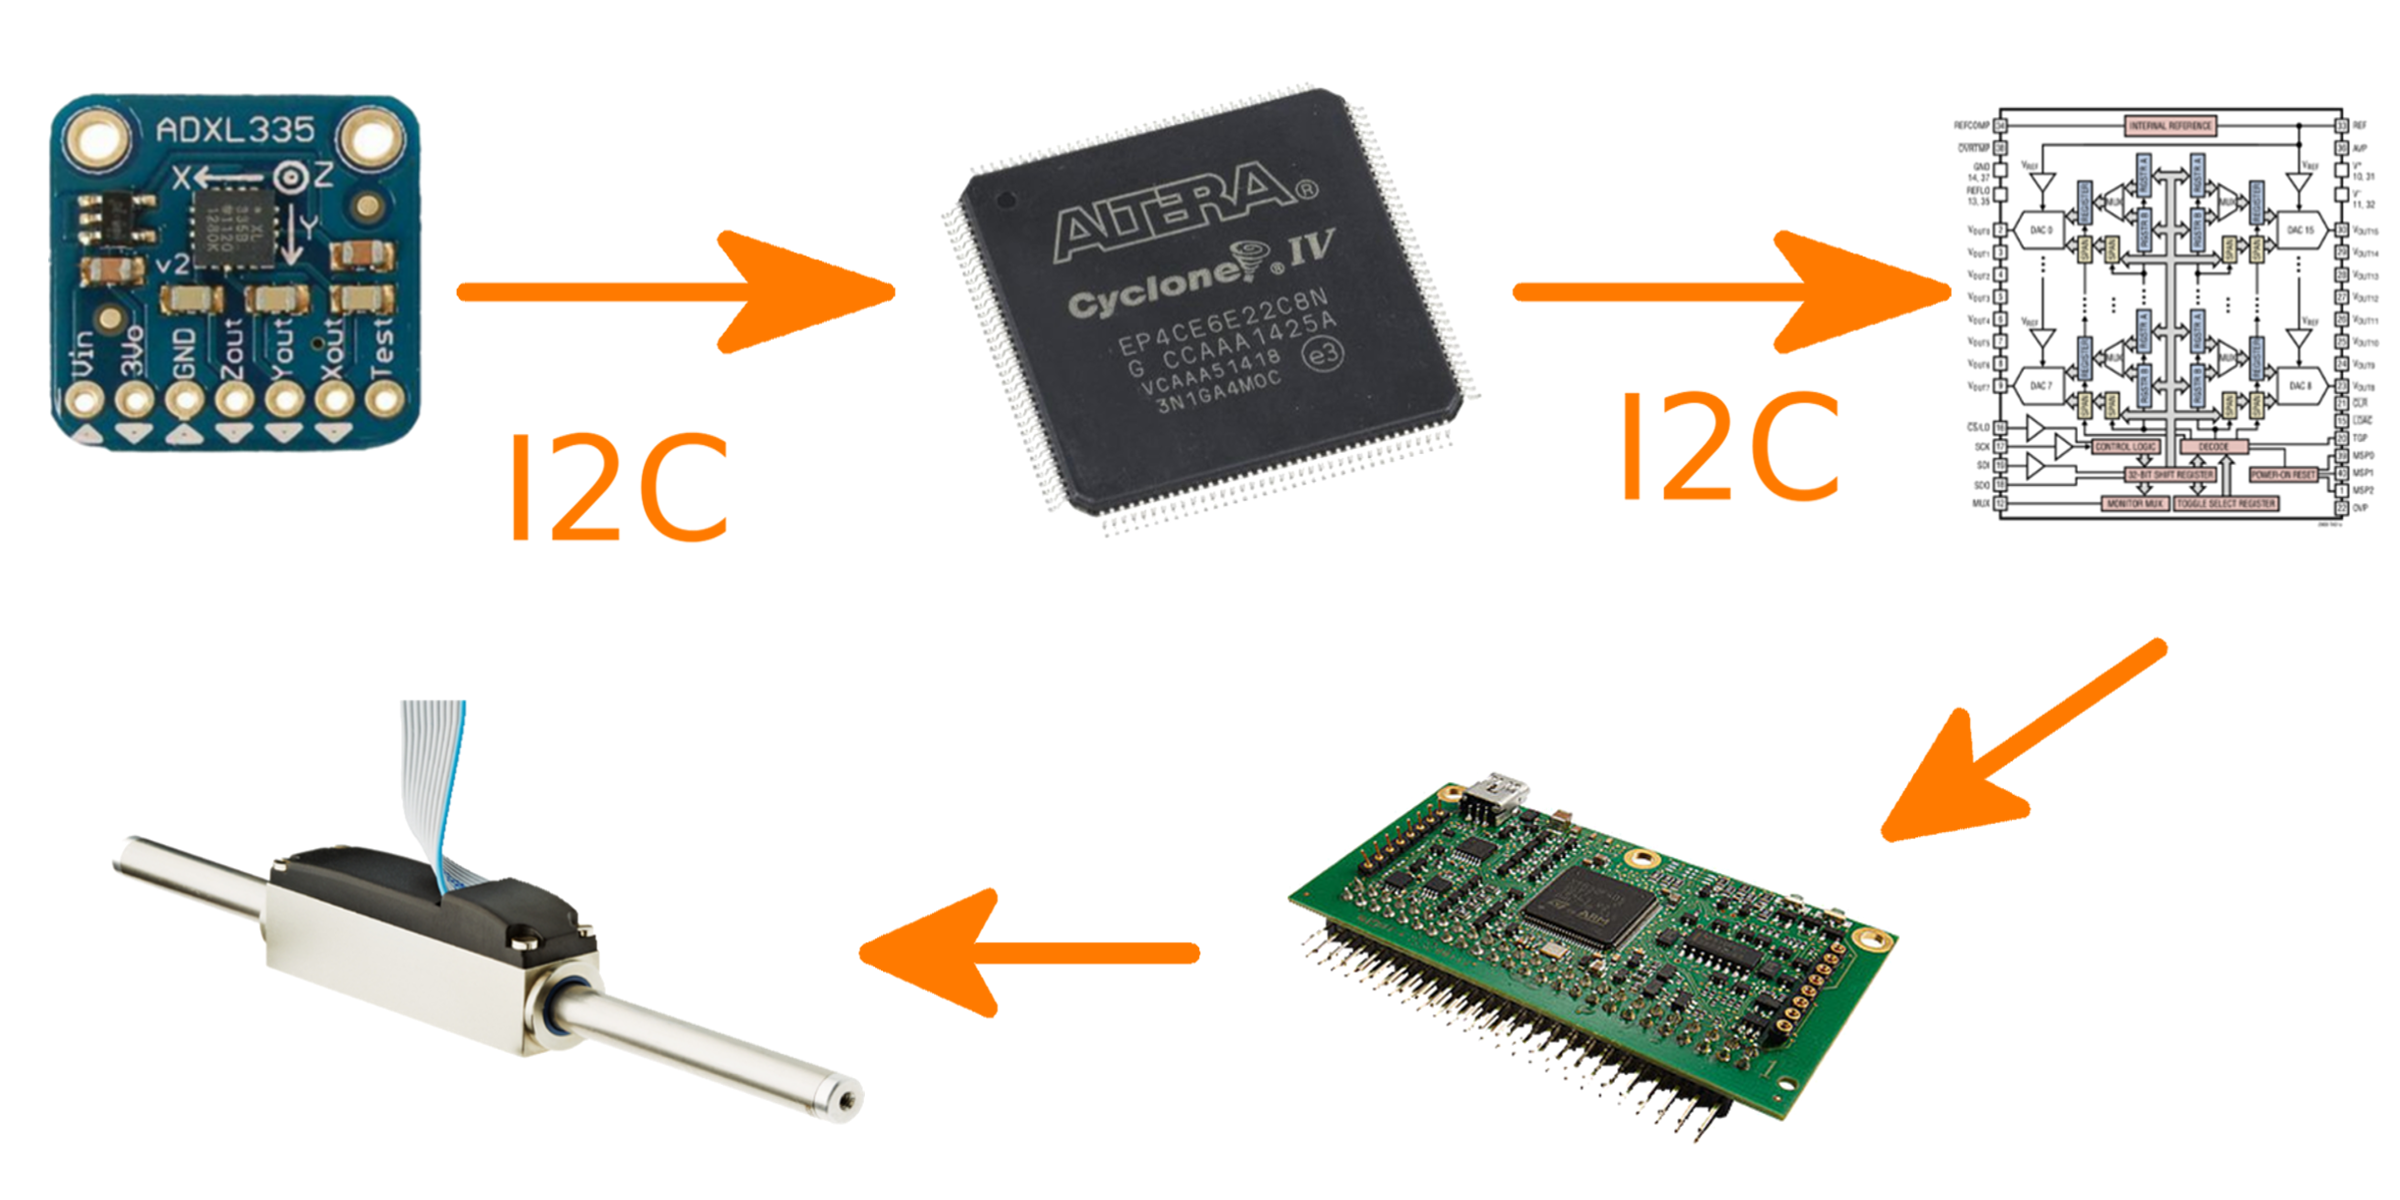
\includegraphics[width=17cm]{CH.png}\hss}\hfill\null
  	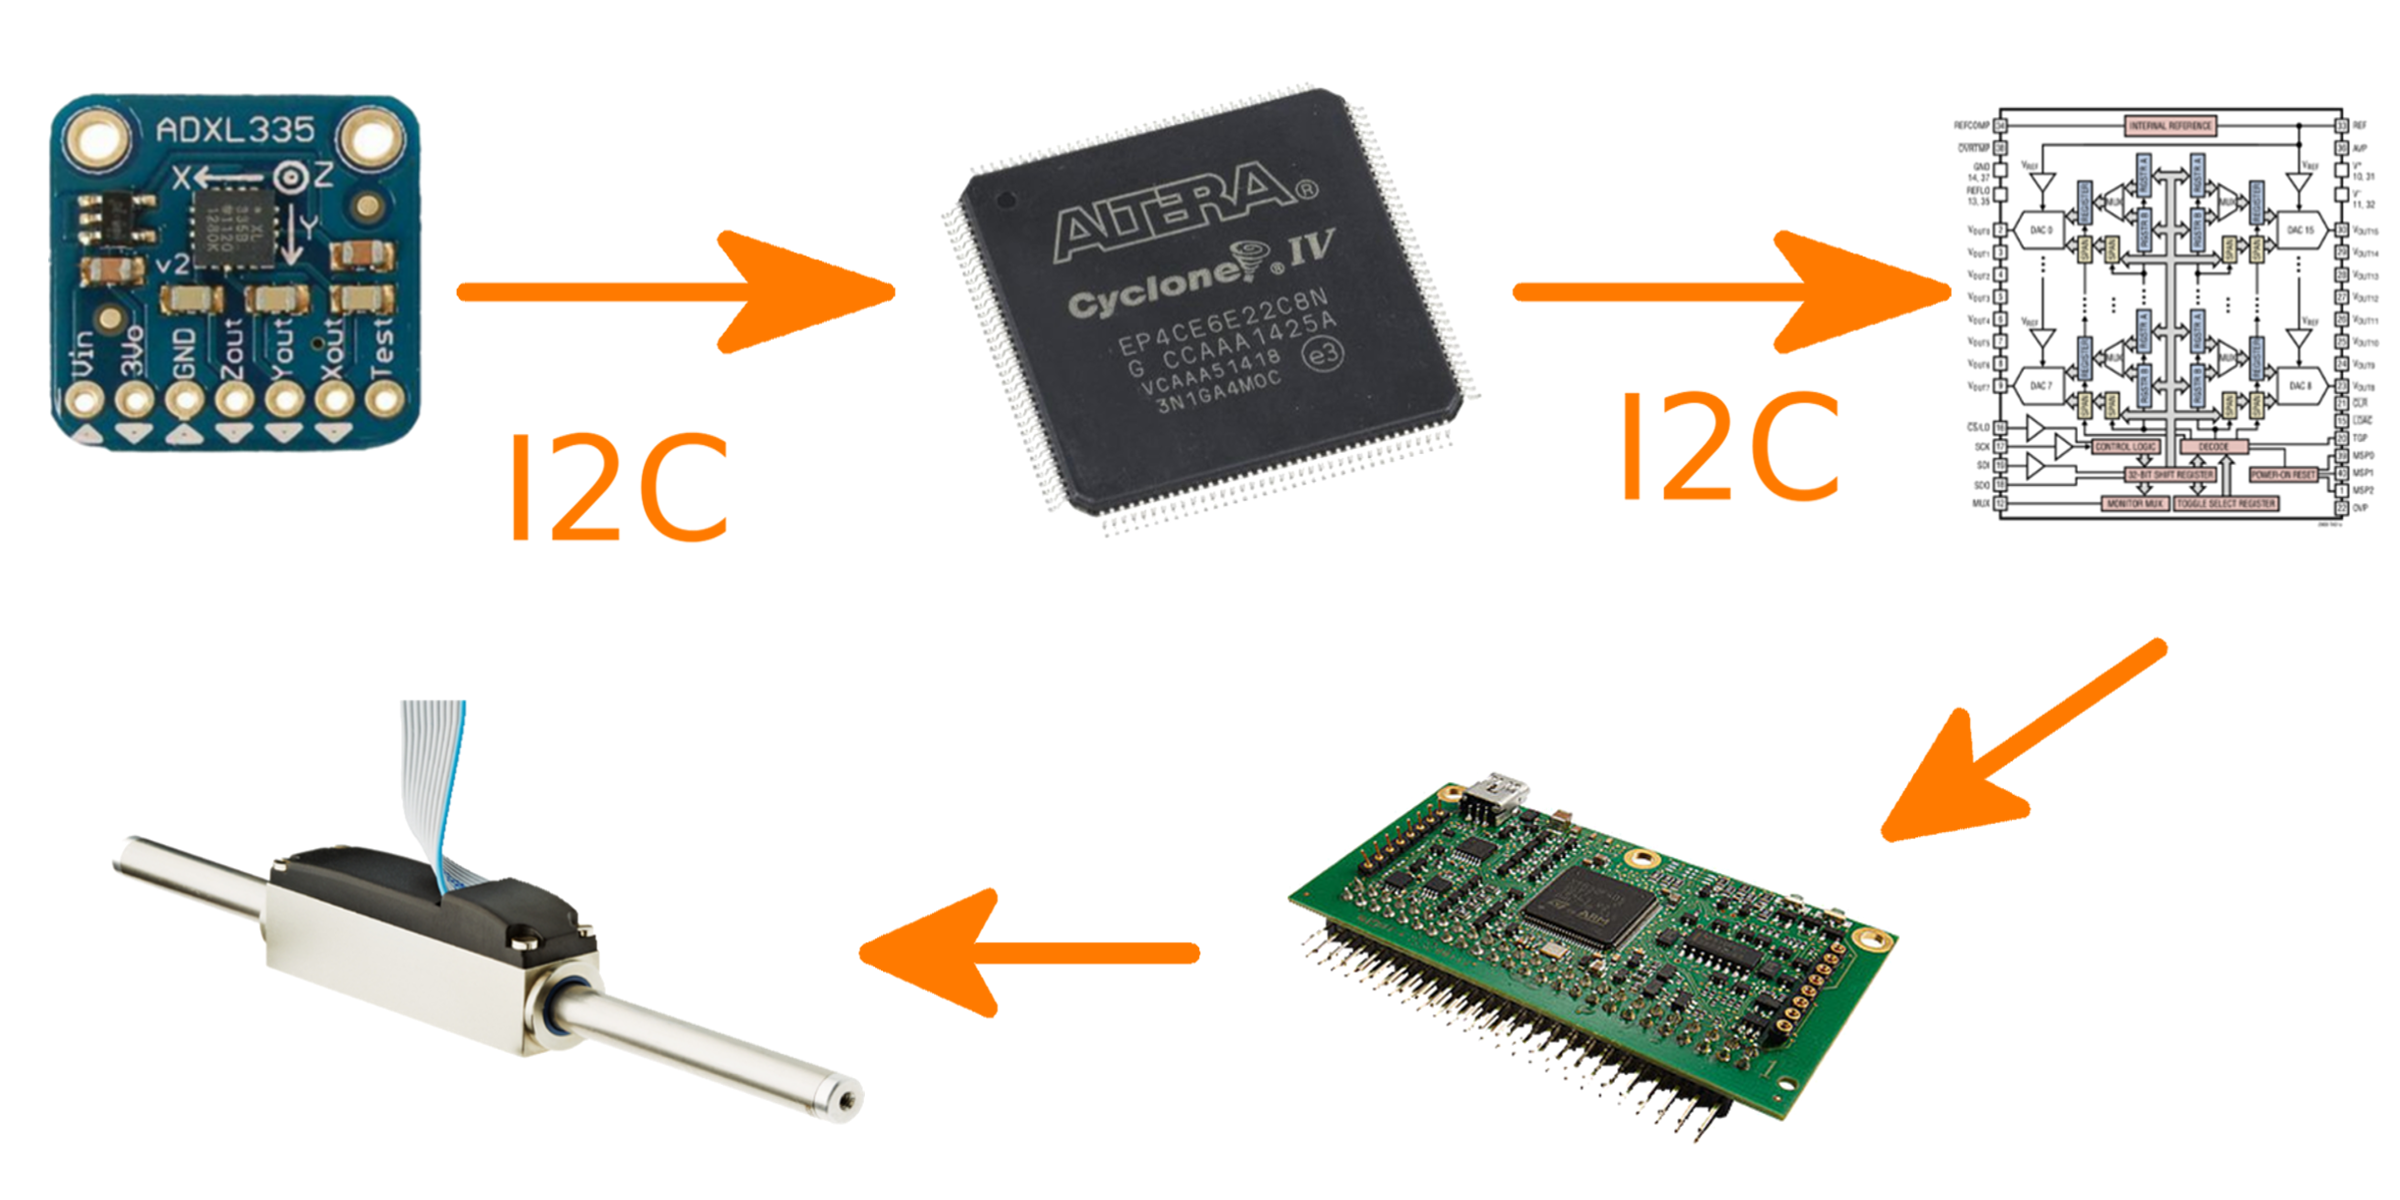
\includegraphics[width=17cm]{CH.png}
    \caption{Chaîne de contôle d'une touche de Piano}
	\end{figure}	
	
	Ainsi, la toute première tâche réalisée fut de mener une étude de cas entre les deux bus de communication à disposition, le bus I2C et le bus SPI, afin de déterminer lequel serait le plus adapter à notre projet.
	
	Cette étude de cas m'a par la suite conduit à éprouver un "hack" sur notre accéléromètre. Notre choix de bus de communication induisant un grand nombre de câble de branchement, que nous souhaitions faire diminuer.
	
	La suite logique à cette étape fut d'étudier le bus de communication sélectionné, afin de l'instancier au sein du projet, en se basant sur le langage VHDL. Ce bus de communication étant présent en deux endroits de la chaîne, entre l'accéléromètre et la carte programmable FPGA et entre cette dernière et notre convertisseur numérique analogique, notre intégration devait répondre aux spécificités des deux cas d'utilisation, afin de ne pas faire doublon dans la mise en place de solution, ainsi que dans les potentielles sources d'erreurs.
	
	Puis, après avoir éprouvé l'échange de données, entre les différentes entités, un filtrage numérique fut intégré à notre carte programmable. Ce filtrage ayant pour but de mettre en place un asservissement numérique sur le contrôle des moteurs.

	Par la suite, différents prototypes de cartes électroniques (PCB) ont dû être réalisés et réévalués tout au long du projet, afin de répondre aux impératifs d'intégration matérielle au sein du piano.
	
	Enfin, une étude de "rétro-engineering" fut menée en salle de test sur des éléments électroniques tiers, fournie par notre partenaire technique, l'entreprise "Faulhaber", afin d'en vérifier le bon fonctionnement, mais également d'en valider le comportement vis-à-vis de l'utilisation souhaitée.
	
	Mais comme expliqué en ce début de partie, ce module, illustré ci-dessus, n'est qu'un douzième du prototype final; ne permettant la récupération et le traitement que d'un seul accéléromètre à la fois et donc, d'une seule touche à la fois.
	
	La maquette à réaliser étant composée de 12 touches, il nous faudra par la suite généraliser notre module afin de récupérer et traiter les informations de nos 12 touches, de manière parallèle.
	Ce travail étant un peu plus complexe que le module précédemment présenté, il demande une refonte d'une partie de la chaîne, vis-à-vis de l'échange de données entre la carte programmable (FPGA) et le convertisseur numérique analogique (CNA).
	
	\chapter{Planning}

	Ci-dessous sont présentés, sous forme de diagrammes de Gant, le calendrier prévisionnel ainsi que le calendrier réel du travail réalisé tout au long du stage.
	On y retrouve un descriptif complet et détaillé des différentes tâches réalisées.
	
	On peut observer sur le calendrier réel que les phases de test, de débug, n'avaient pas été prises en compte lors de l'établissement du calendrier prévisionnel.
	À l'avenir, ces tâches ne seront plus sous-estimées, étant donné le caractère important de celles-ci, du fait de leur capacité à bloquer l'avancement d'un projet et induire des retards plus ou moins importants.
	
	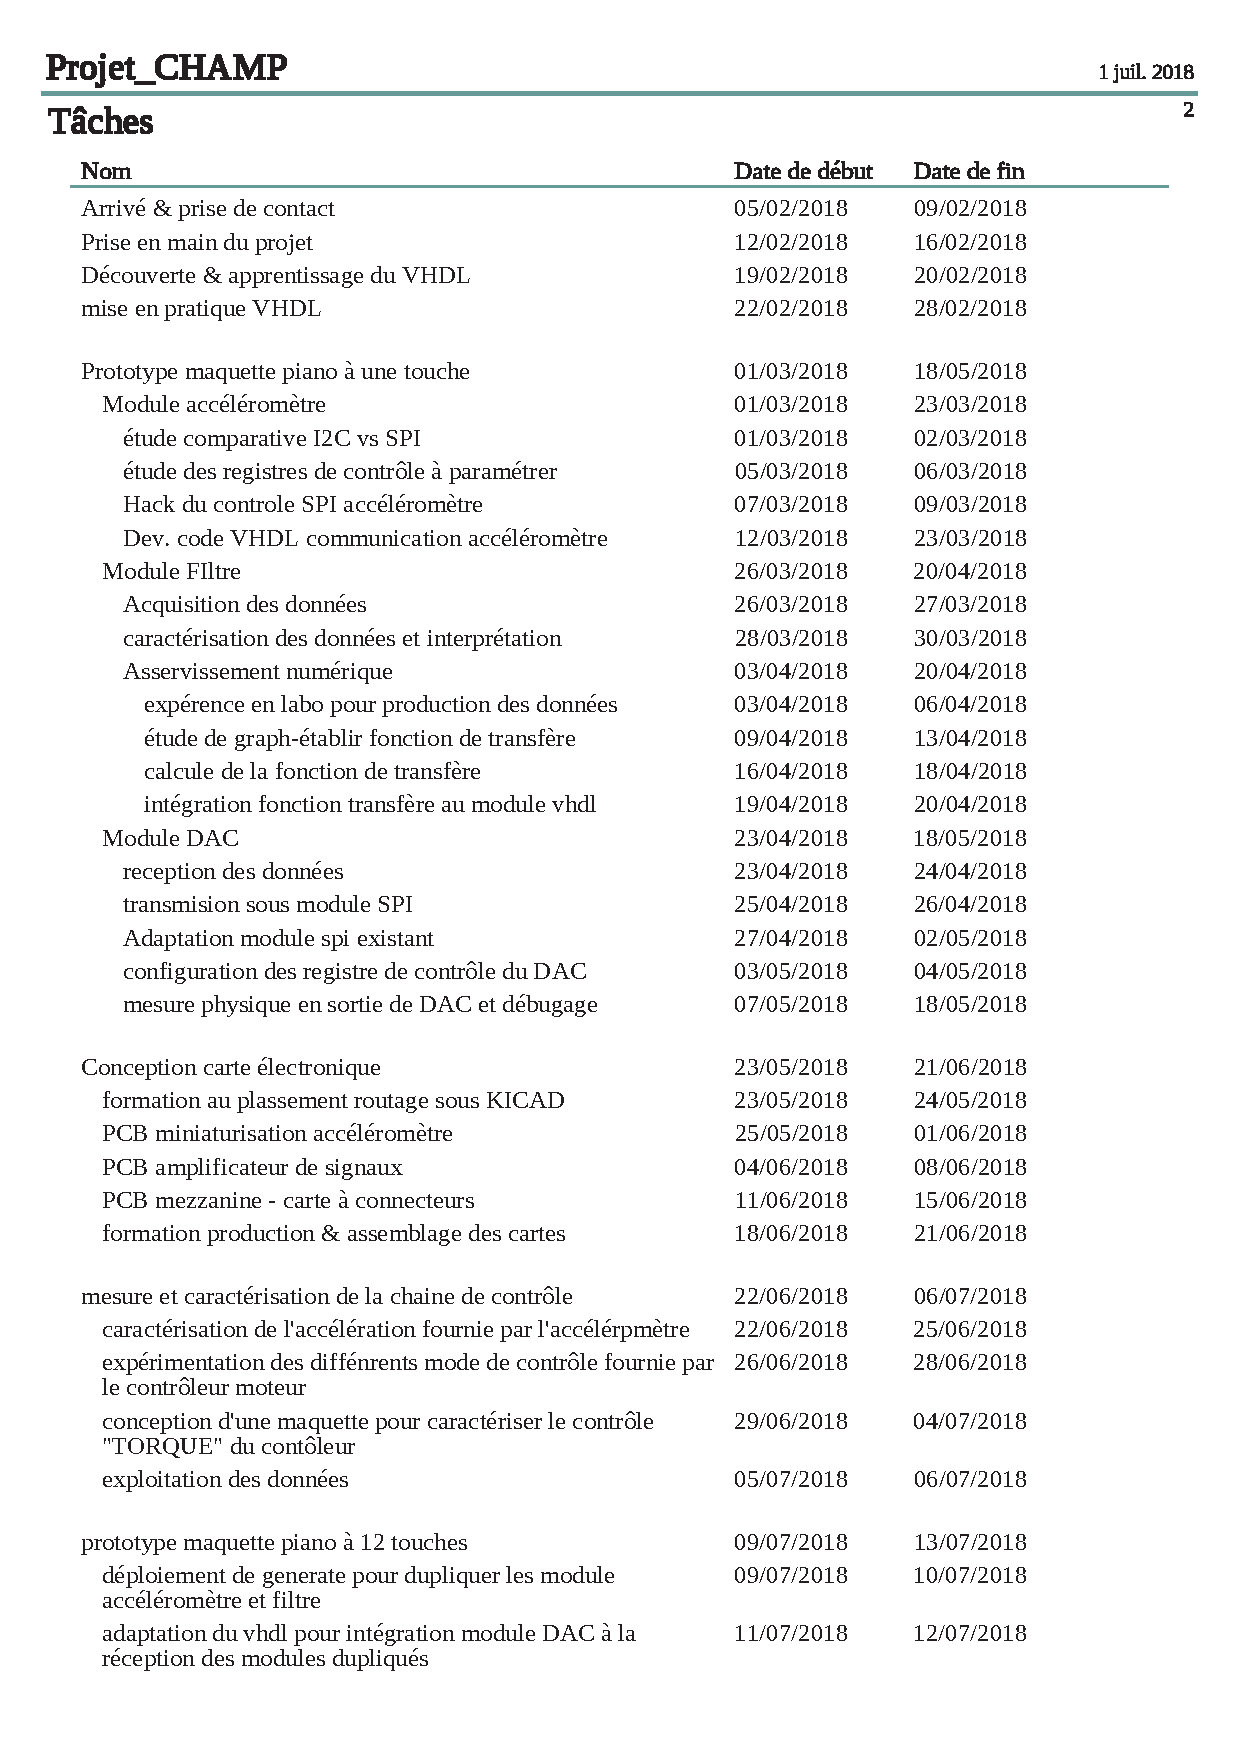
\includepdf[scale=1, pages=-]{calendrier_Previsionnel_defA}
	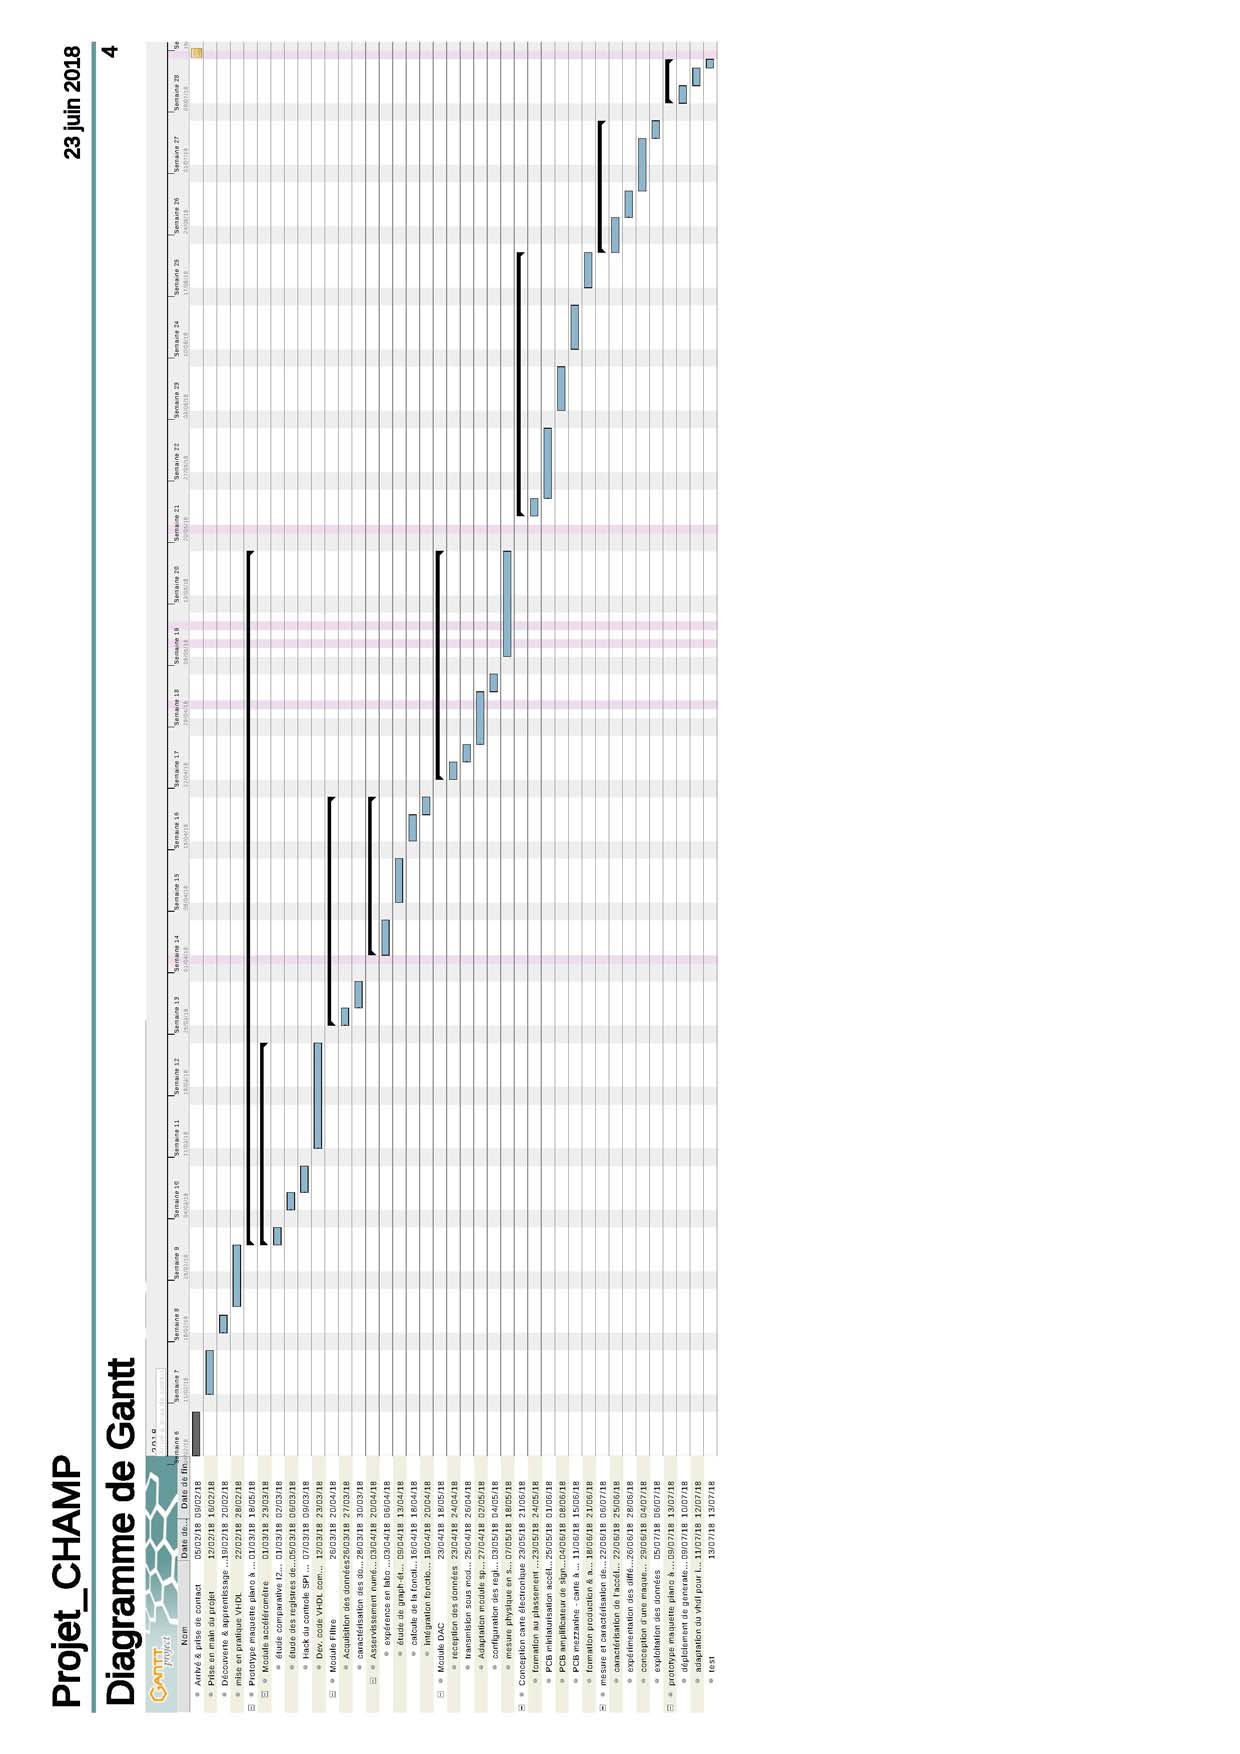
\includepdf[scale=1, pages=-]{calendrier_Previsionnel_defB}
	
	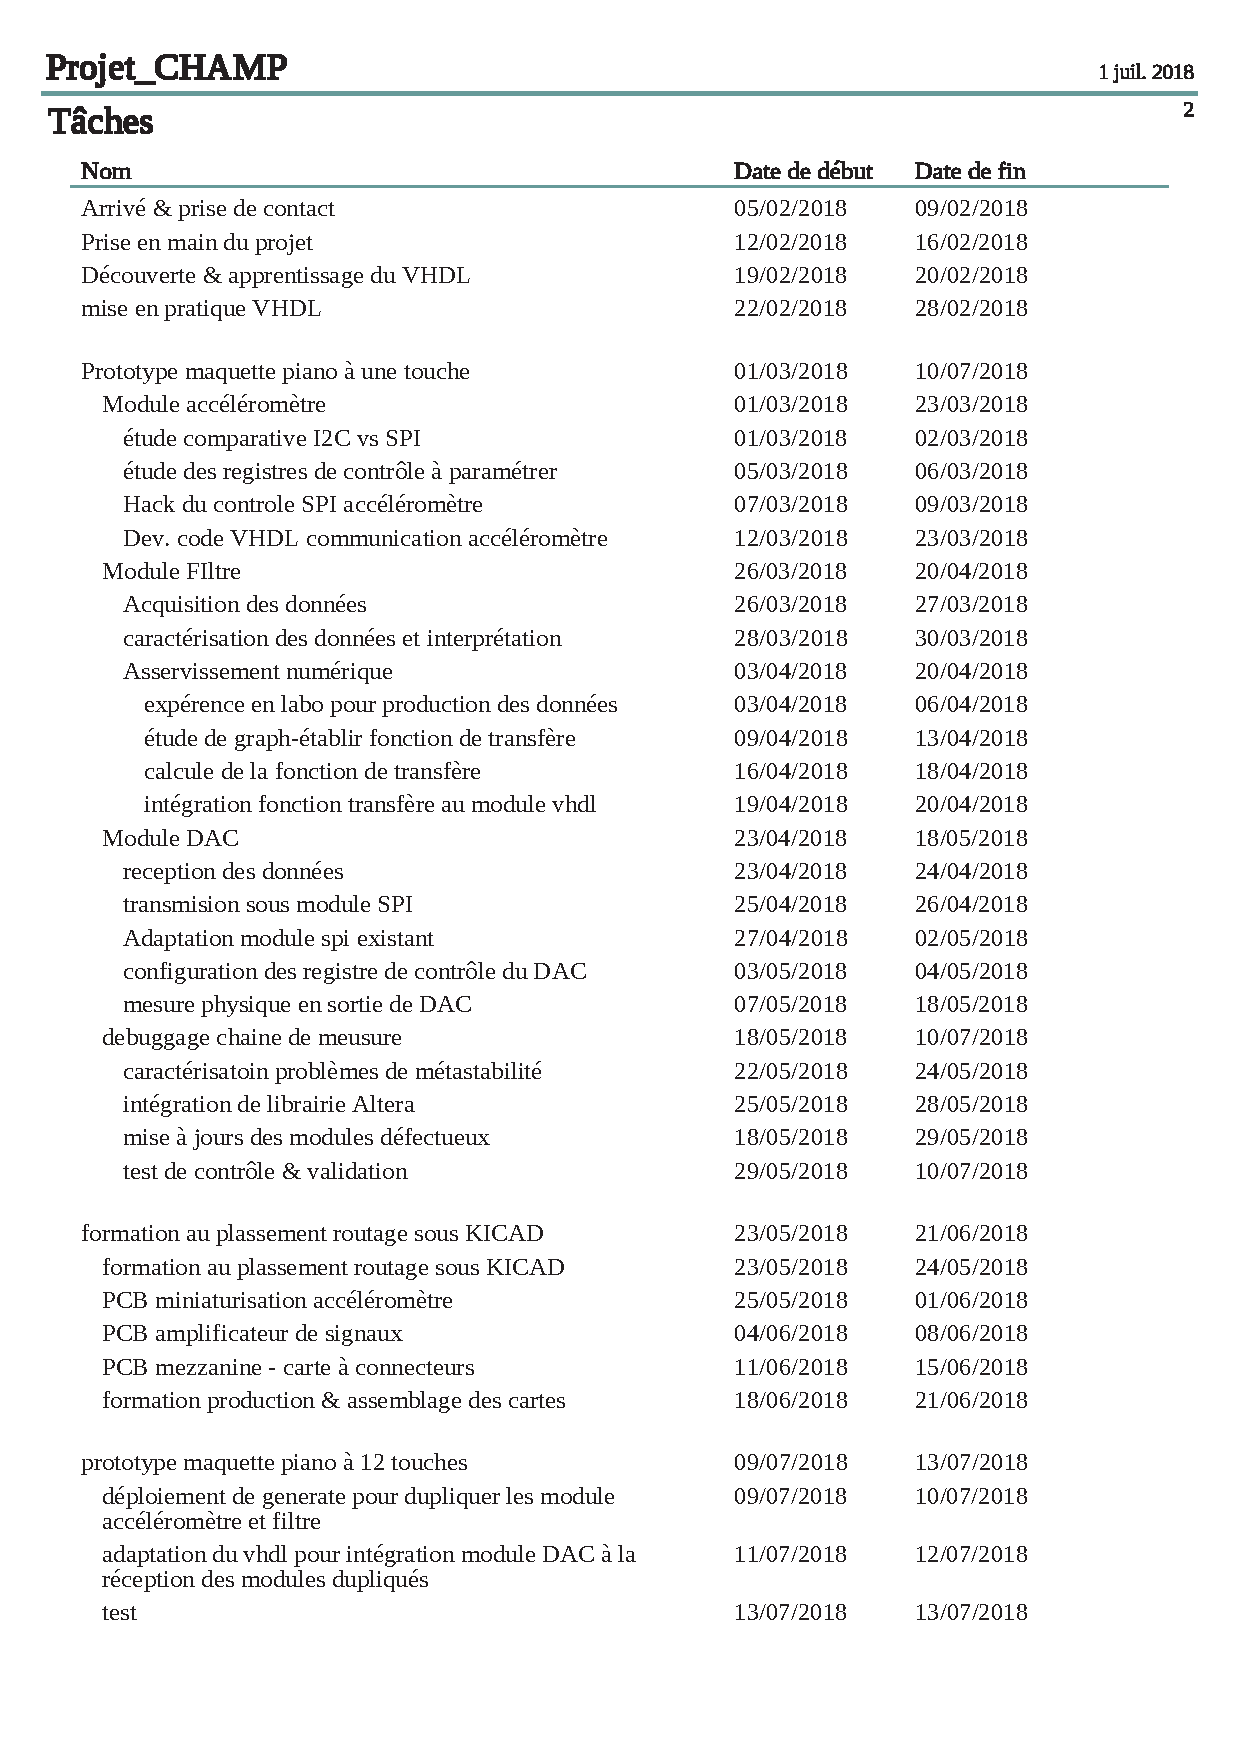
\includepdf[scale=1, pages=-]{calendrier_reel_defA}
	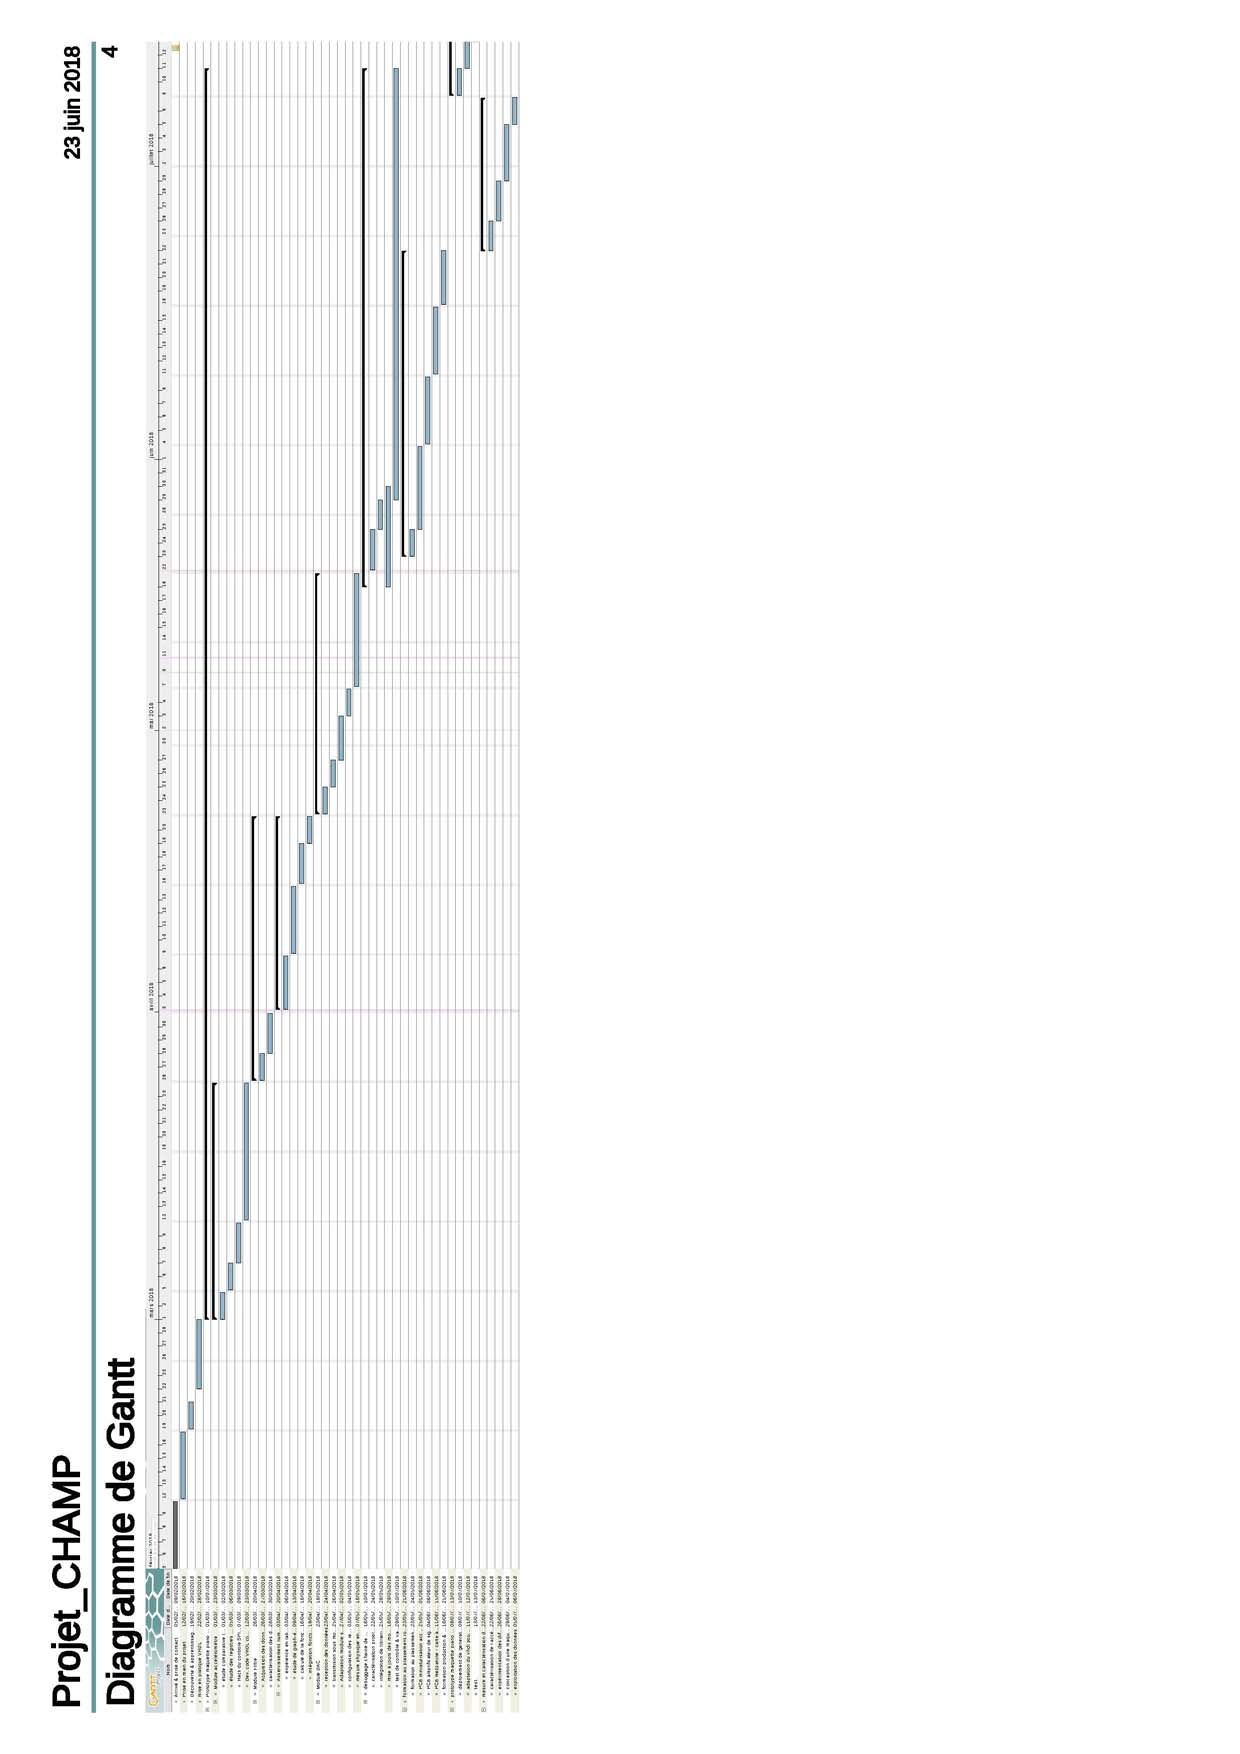
\includepdf[scale=1, pages=-]{calendrier_reel_defB}	
	
	
	
	
%--------------------------------------------------------------------------------------
%
%	Présentation et Détail des travaux Réalisés durant le stage
%
%--------------------------------------------------------------------------------------
	
	\part{Réalisation de la chaîne de contrôle}	
	
	Maintenant que le cadre du projet a été présenté, ainsi que les objectifs visés au travers de cette preuve de concept, nous allons maintenant nous concentrer sur la réalisation pratique, ainsi que sur les aspects techniques du projet.
	
	Ainsi, au sein de cette partie, nous allons aborder la conception de la première maquette de notre projet, cette dernière ayant pour rôle de mettre en situation l'action d'une touche; représentant l'action primaire d'un piano, une action sur une touche, permettant la frappe d'une corde par un marteau. Par la suite, lorsque cet aspect sera maîtrisé, nous pourrons passer au développement d'une deuxième maquette se basant sur un ensemble plus complet d'une douzaine de touches, afin de disposer d'un jeu sur une octave et demie.
	
		\chapter{La chaîne de contrôle}
		
		Cherchant à mettre en place une nouvelle mécanique interne afin de permettre la frappe d'une corde par un marteau, suite à une pression sur une touche de piano, nous avons cherché à développer une nouvelle chaîne de contrôle électronique.
		Mais comme expliqué précédemment, nous cherchons à proposer une nouvelle expérience de jeu aux pianistes, sans altérer l'expérience utilisateur liée à la pratique de l'instrument. C'est pourquoi notre nouvelle chaîne de contrôle ne vient pas remplacer la mécanique interne, dite "classique" du piano; cette dernière venant se "greffer" autour de l'ancienne, tout en nécessitant une adaptation de l'existante.
		
		Notre chaîne de contrôle électronique se compose comme suivant:
		\begin{itemize}
			\item Un accéléromètre, mesurant l'accélération du marteau, suite à une pression sur une touche du piano.
			\item Une carte programmable FPGA, nous permettant d'effectuer un traitement du signal sur nos données renvoyées par notre accéléromètre.
			\item Un convertisseur numérique analogique (CAN), pemettant de convertir le signal numérique fournit par le FPGA, en un signal analogique (dans notre cas, un niveau de tension)
			\item Un contrôleur moteur, assurant le contrôle en triphasé de notre moteur brushless.
			\item Un moteur brushless, assurant le rôle de marteau, afin de frapper une corde.
		\end{itemize}
		
		\begin{figure}[!ht]
    \center
    %\hfill\hbox to 0pt{\hss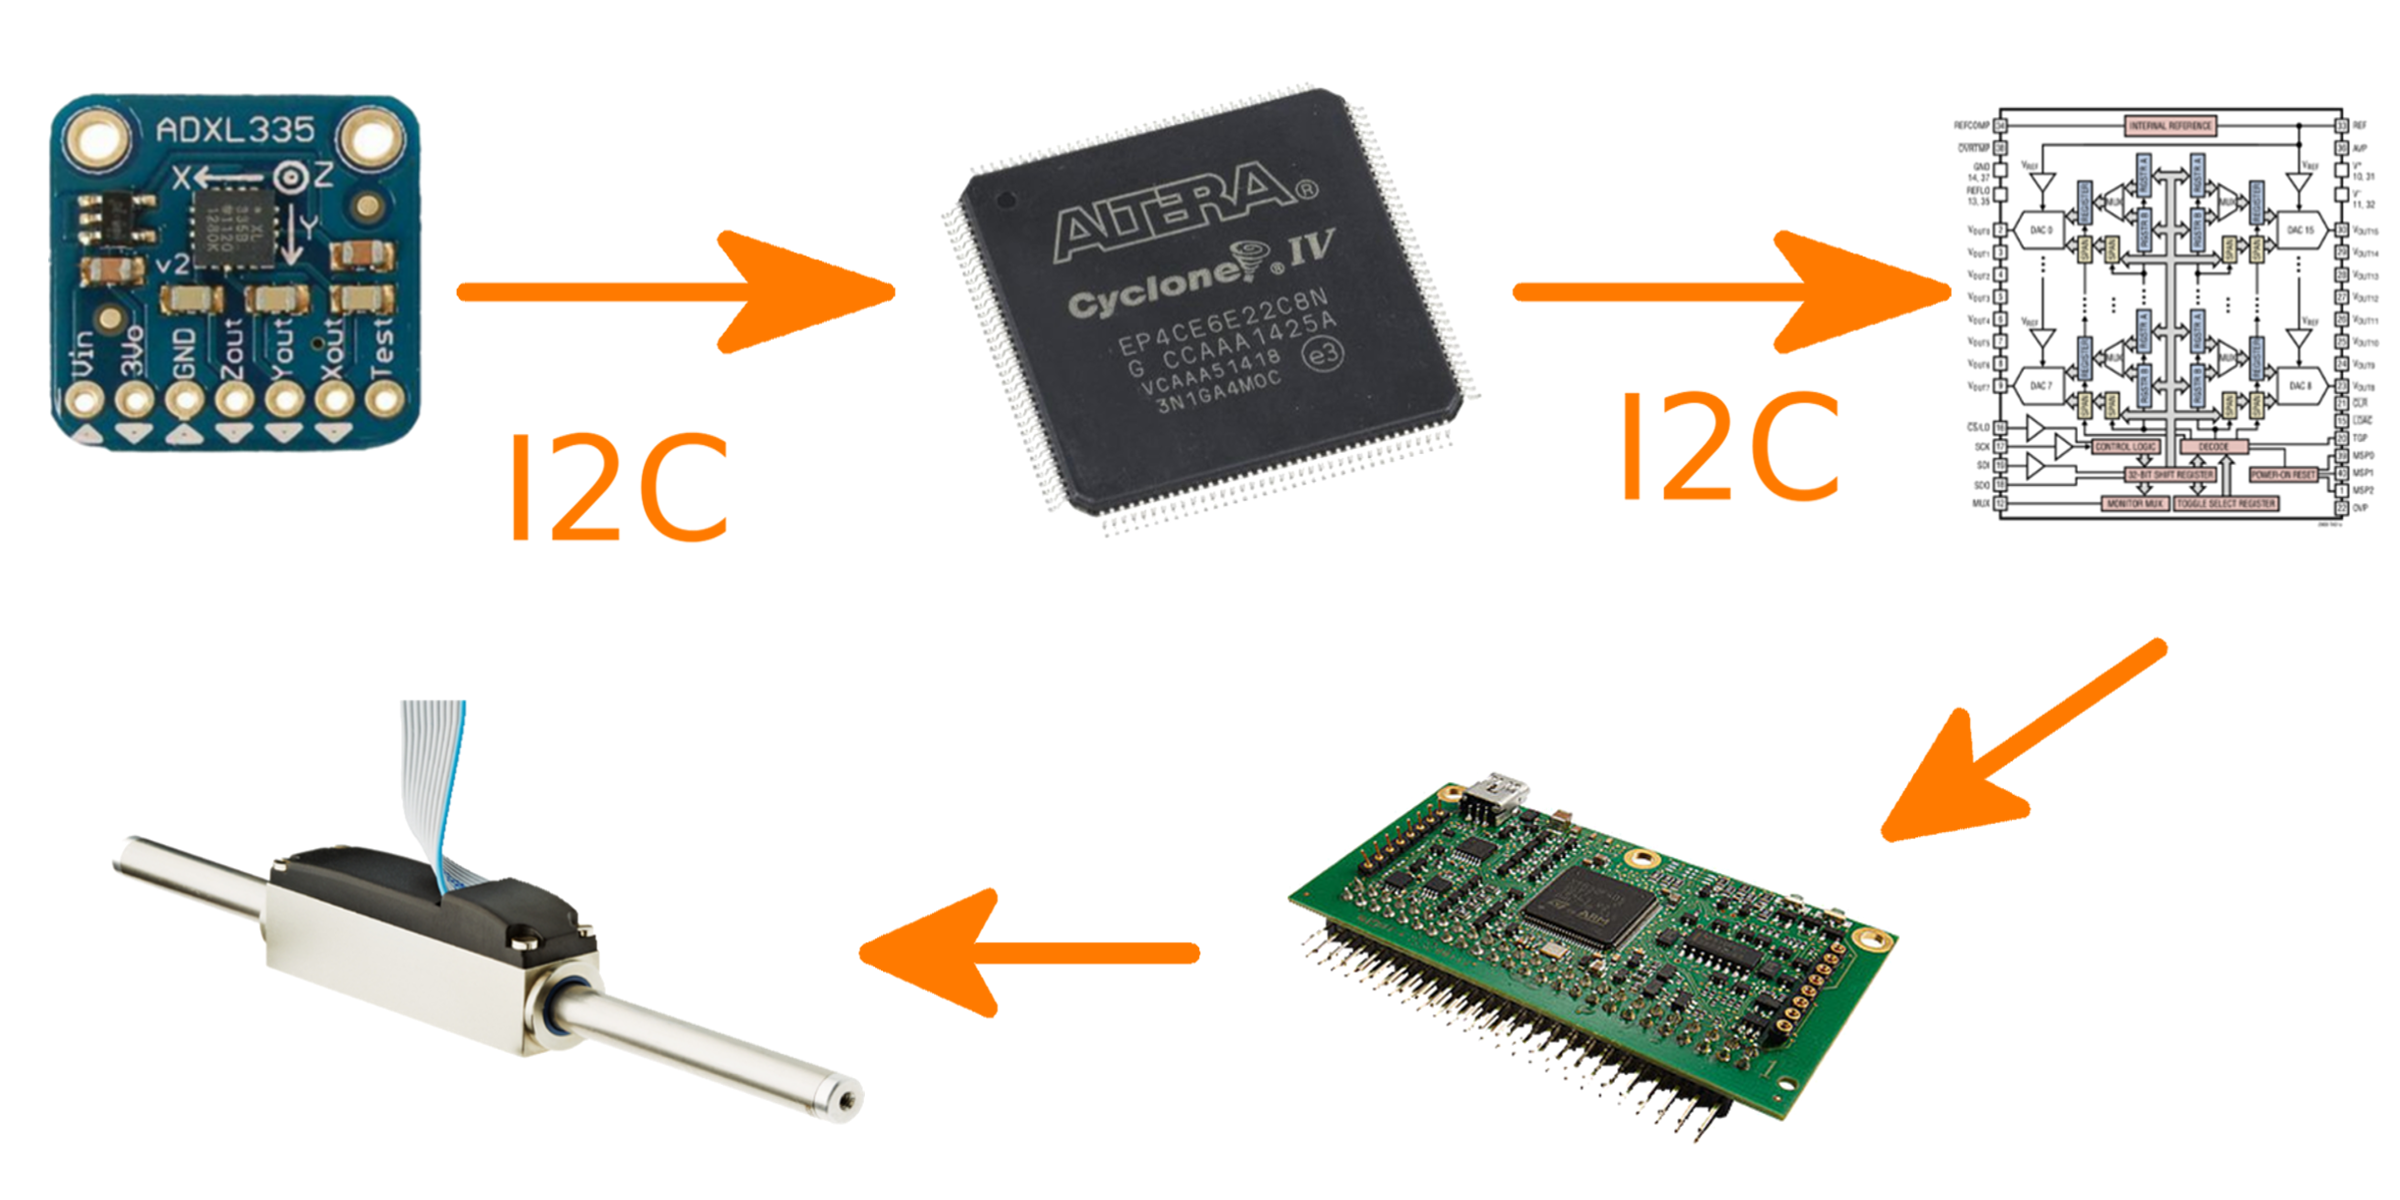
\includegraphics[width=17cm]{CH.png}\hss}\hfill\null
  	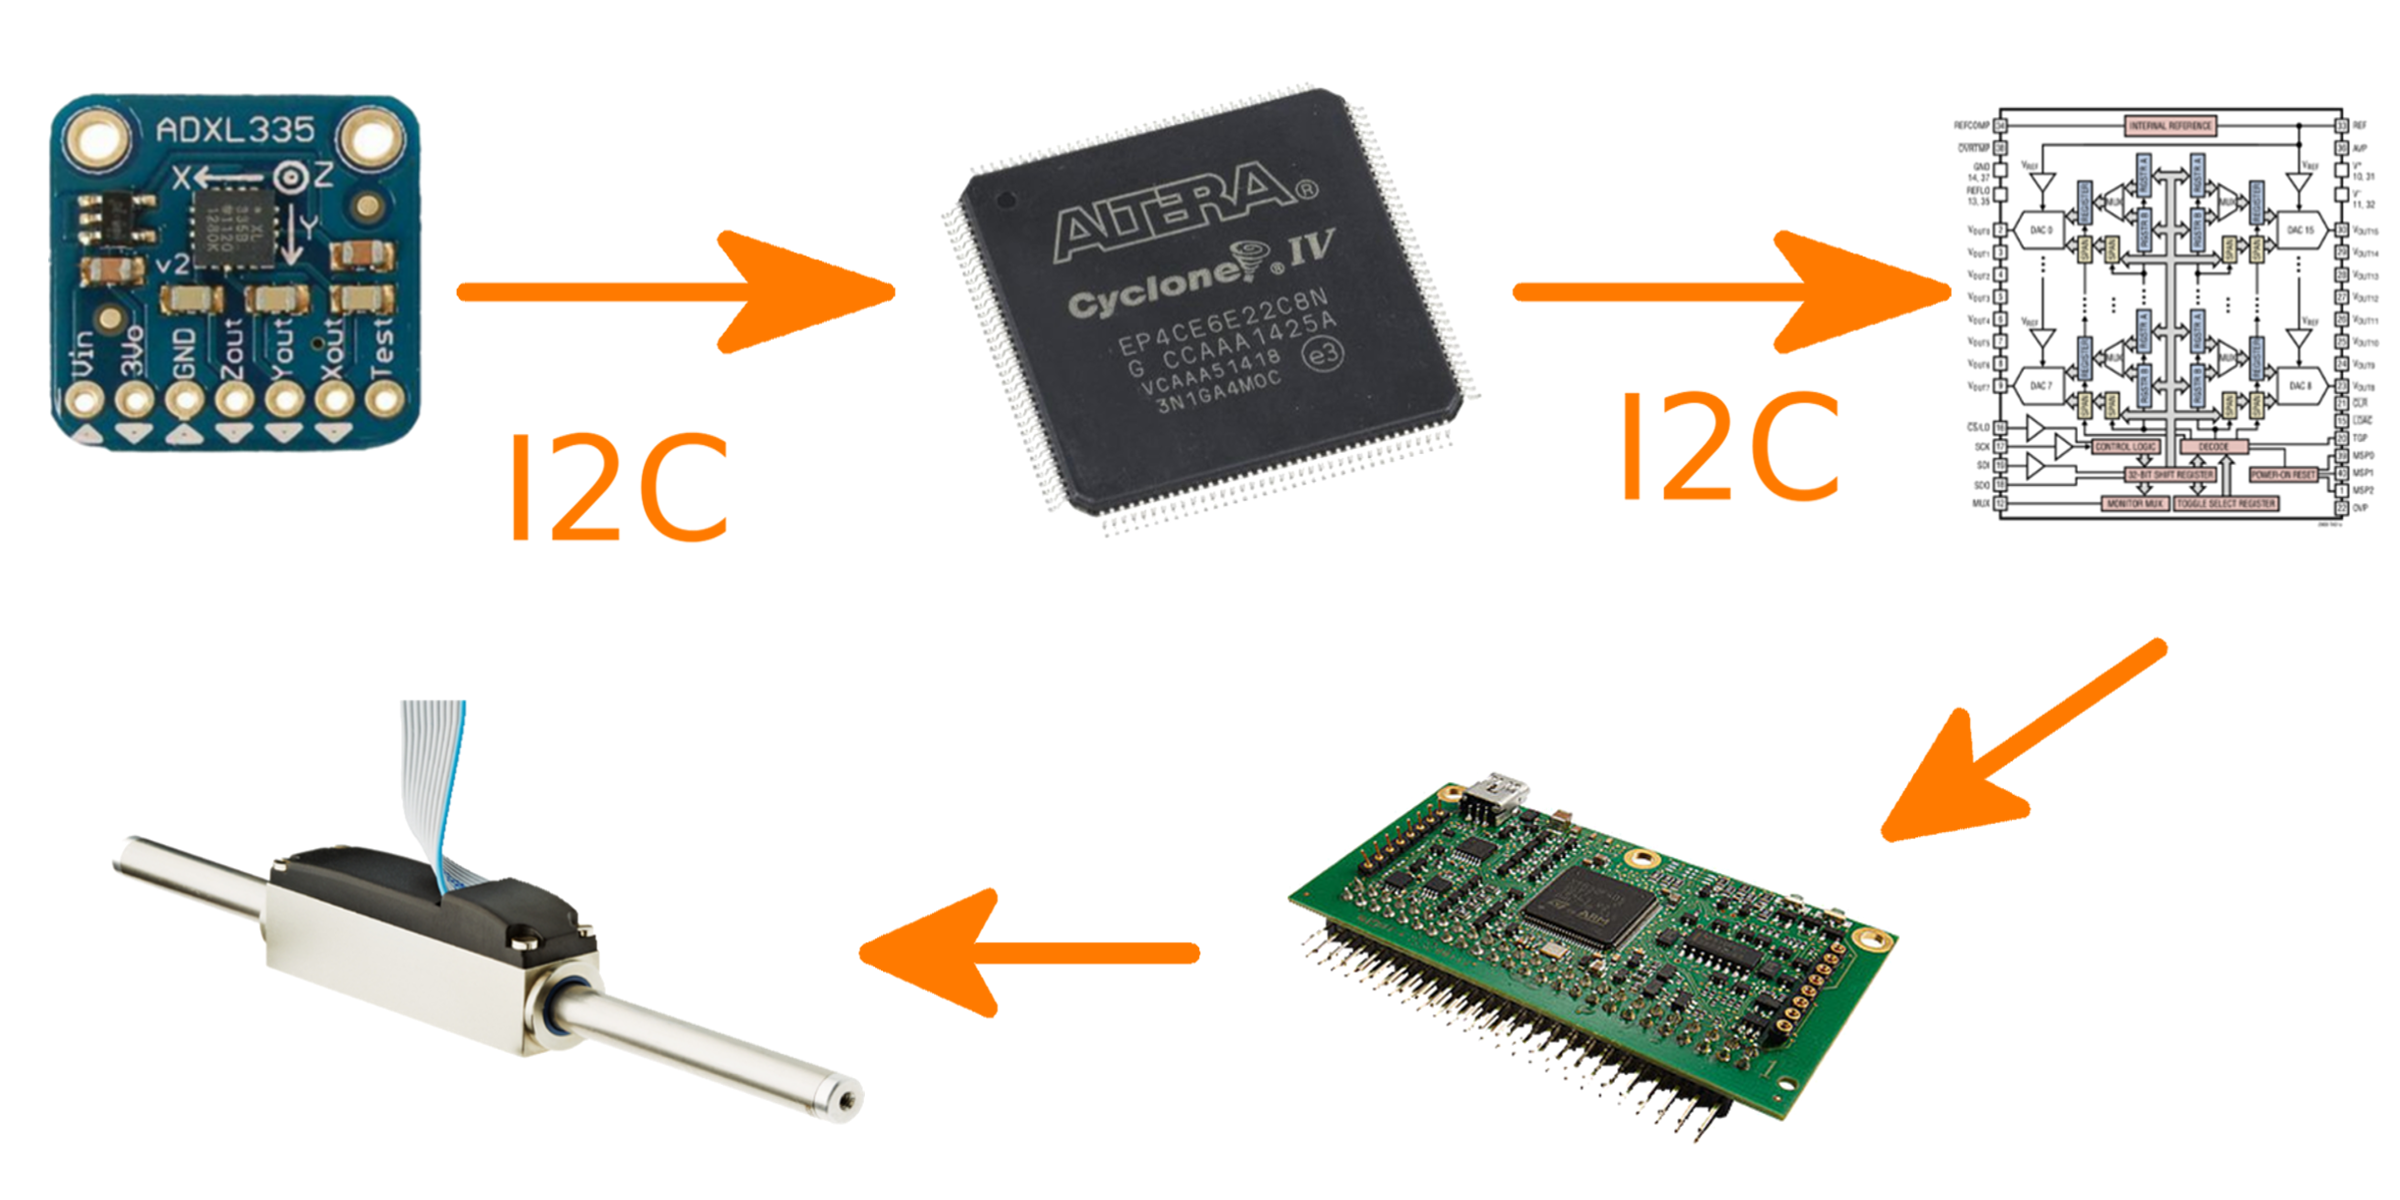
\includegraphics[width=17cm]{CH.png}
    \caption{Chaîne de contôle d'une touche de Piano}
	\end{figure}
	
			\section{l'accéléromètre}
						
			Comme nous l'avons vu lors de la précédente partie, la réalisation d'un système d'assistance et d'asservissement d'une mécanique de piano à queue induit l'appel à des technologies de "pointe"; technologie que nous retrouvons et côtoyons au quotidien au travers de nos smartphones, notamment celle nous permettant de mesurer une accélération (technologie qui sera une composante principale de notre projet).
 
La mesure de l'accélération est la composante clef de notre projet, étant donné que ce seul élément rend possible la mesure de l'accélération (sur trois axes x,y,z) de la touche jouée par le pianiste, ainsi que la mise en place de la boucle d'asservissement contrôlant les moteurs devant actionner les marteaux en coton frappant les cordes.

			%\subsubsection{Matériel utilisé}
			
			Pour ce projet, une première maquette utilisant des composants électroniques analogiques fut réalisée, se basant sur le modèle de la figure (dernière figure). Ce prototype avait pour but de montrer la manière de procéder et de vérifier le postulat de départ quant à la faisabilité du projet.
 
% PHOTO de la maquette initiale de Hervé
 
Suite à mon arrivée au sein du projet "CHAMP", j'ai commencé le développement de la nouvelle maquette (toujours basée sur le même schéma de fonctionnement) qui est maintenant basée sur des composants électroniques numériques.
 
Le capteur numérique utilisé, et choisi par l'équipe qui a initié le projet, est l'accéléromètre ADXL355 du fabriquant "ANALOG DEVICE". Ce composant nous permet de mesurer une accélération sur 3 axes (x,y,z) avec une précision de +/- 8 fois la force gravitationnelle.
 
Le module ADXL355 permet l'échange de données avec notre FPGA (unité de traitement et de calcul) via des transmissions série synchrones. Il peut ainsi communiquer via deux protocoles de communication, le SPI ou le protocole I2C.
			
			\section{le FPGA}
			
			Concernant l'utilisation d'une carte programmable munie d'un FPGA pour le projet, cet élément fut un choix technique pris par les responsables du projet, étant donné l'utilisation majeure de ce type de technologie au sein du laboratoire.
			
			Ainsi, la carte programmable utilisé est une DE2-115, un kit de développement et de prototypage, embarquant une large gamme de technologie utilisable, dont voici une liste exhaustive. On retrouve à disposition un FPGA (35.000 LE) comme coeur, de plusieurs types de mémoire (SRAM, SDRAM et Flash), de convertisseurs audio, vidéo et TV, ainsi que d'interfaces IrDA, Ethernet et USB. De plus, la carte est munie d'afficheurs LED et LCD et d'un grand nombre de boutons poussoirs ainsi que d'interrupteurs.
			
			L'utilisation de ce genre de kit permet une grande souplesse lors du développement étant donné la grande disponibilité de technologies par défaut. Ainsi, l'intégration de nouvelles fonctionnalités au fur et à mesure du projet en devient plus aisé. C'est une fois le prototypage fini, que nous concevrons une carte sur mesure, avec seulement les technologies requises afin de minimiser les coûts de fabrication et d'encombrement.
			
			\section{Le convertisseur analogique numérique}
			
			L'utilisation du Convertisseur Numérique Analogique (CNA) fut également un choix imposé par le laboratoire.
			Ce convertisseur nous permet de transformer le signal numérique provenant de notre FPGA, en un signal analogique, à destination de notre contrôleur moteur.
			
			Ainsi le choix du laboratoire s'est porté sur le CNA "LTC 2668" fabriqué par Analog Device.
			Ce dernier disposant d'une entrée de signal numérique sur un mot de 16 bits non signé, de plus plusieurs niveaux de tension de sortie possibles, [0V; 5V], [0V; 10V], +-2.5V, et enfin le mode qui nous intéresse, +-10 volts, étant donné que notre contrôleur moteur est contrôlé avec un niveau de tension variant entre +-10 volts.
	
			\section{Le contrôleur moteur et le moteur brushless}
			
			À propos du choix du contrôleur moteur et du moteur brushless, le choix du laboratoire s'est porté sur des moteurs en translation "LM1247\_11\_FMM" fabriqués par l'entreprise Faulhaber. Ce dernier est le seul fabriquant au monde à produire ce genre de moteur, avec un contrôleur offrant divers modes de contrôle.
			
			
		\chapter{Accéléromètre, du produit au besoin}
			
			\section{Accéléromètre \& choix du protocole de communication}
				Comme nous l'avons vu plus tôt, notre accéléromètre peut être utilisé avec les deux protocoles de communication suivant: le bus SPI ainsi que le bus I2C. Afin de déterminer quel bus de communication nous devons utiliser, nous avons commencé par effectuer un comparatif des deux technologies, pour déterminer lequel serait le plus en adéquation avec nos besoins.
				
			\subsection{Bus SPI}
			
			Une Liaison SPI (Serial Peripheral Interface) est un bus de données synchrone baptisé par Motorola, opérant en Full-Duplex et qui peut transférer des données sur de courtes distances à des vitesses élevées. Les circuits communiquant selon un schéma Maître/Esclave, où le maître s'occupe totalement de la communication. Plusieurs esclaves peuvent coexister sur un même bus; dans ce cas, la sélection du destinataire se fait par une ligne dédiée entre le maître et l'esclave appelée "Chip Select" (CS) ou Slave Select (SS).
 
			\subsubsection{Principe de fonctionnement}
			
			Durant le transfert de données, le dispositif peut travailler soit en maître, soit en esclave. L'interface SPI permet de connecter un ou plusieurs esclaves à un seul maître via le même bus.
			
	\begin{figure}[!ht]
    \center
    %\hfill\hbox to 0pt{\hss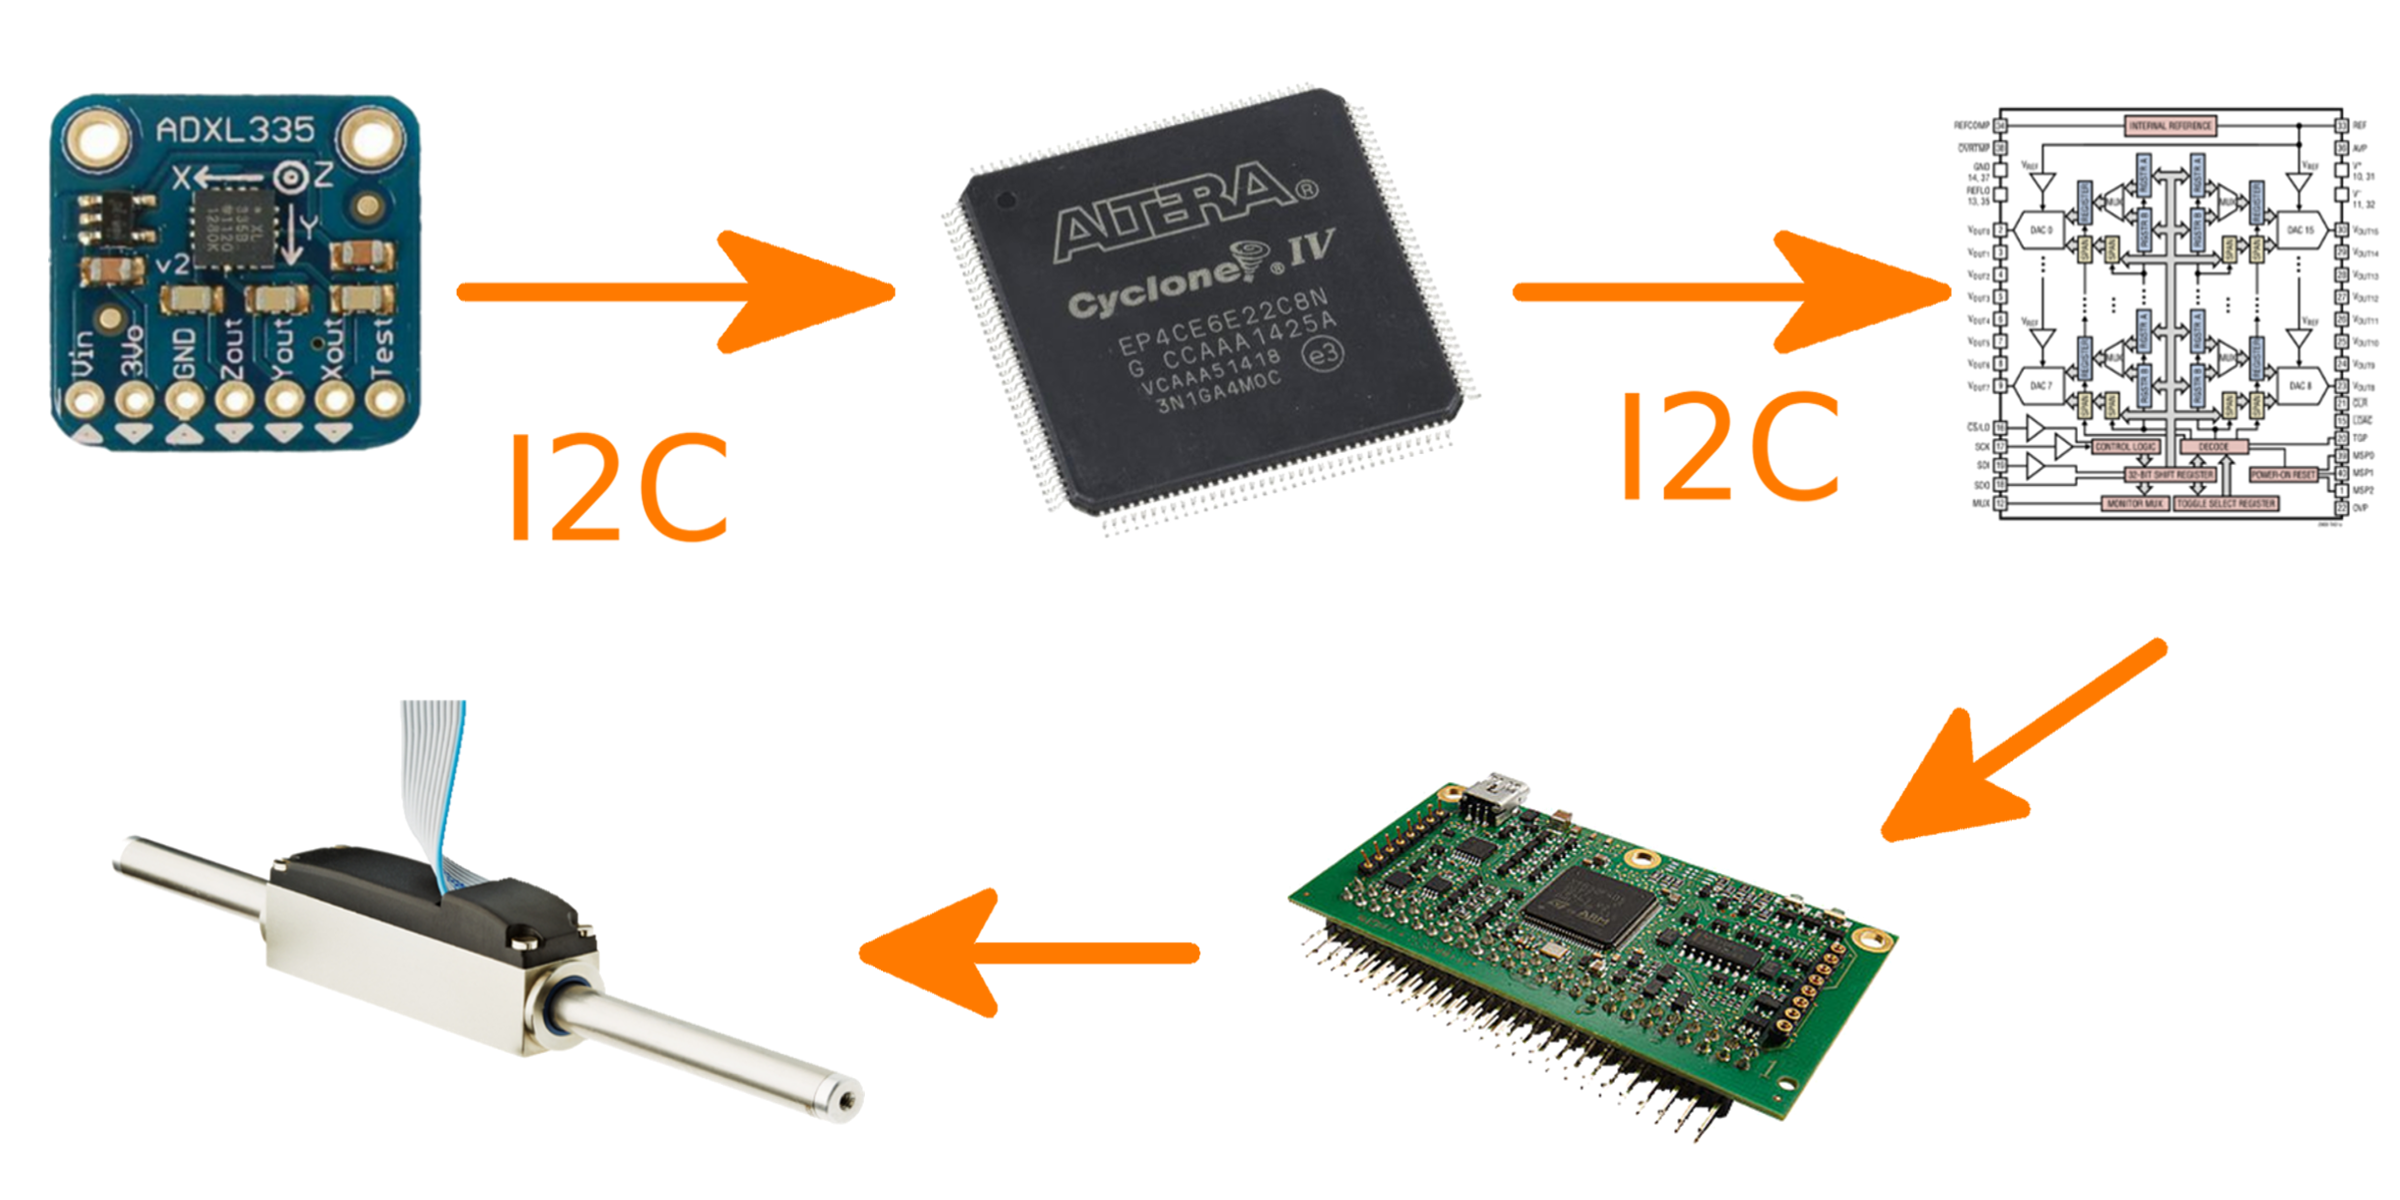
\includegraphics[width=17cm]{CH.png}\hss}\hfill\null
  	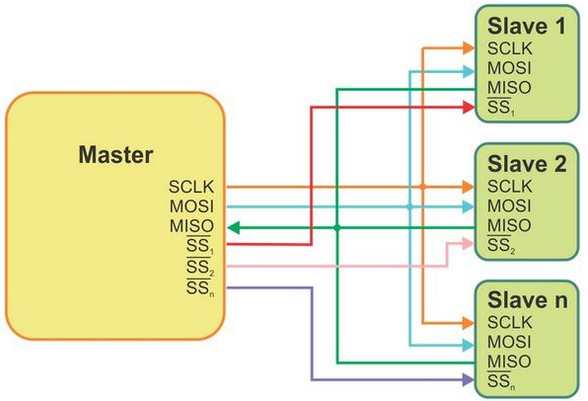
\includegraphics[width=9cm]{SPI1.png}
    \caption{SPI shema block}
	\end{figure}	
 
 
	Le bus SPI utilise quatre signaux logiques :
 
	\begin{figure}[!ht]
    \center
    %\hfill\hbox to 0pt{\hss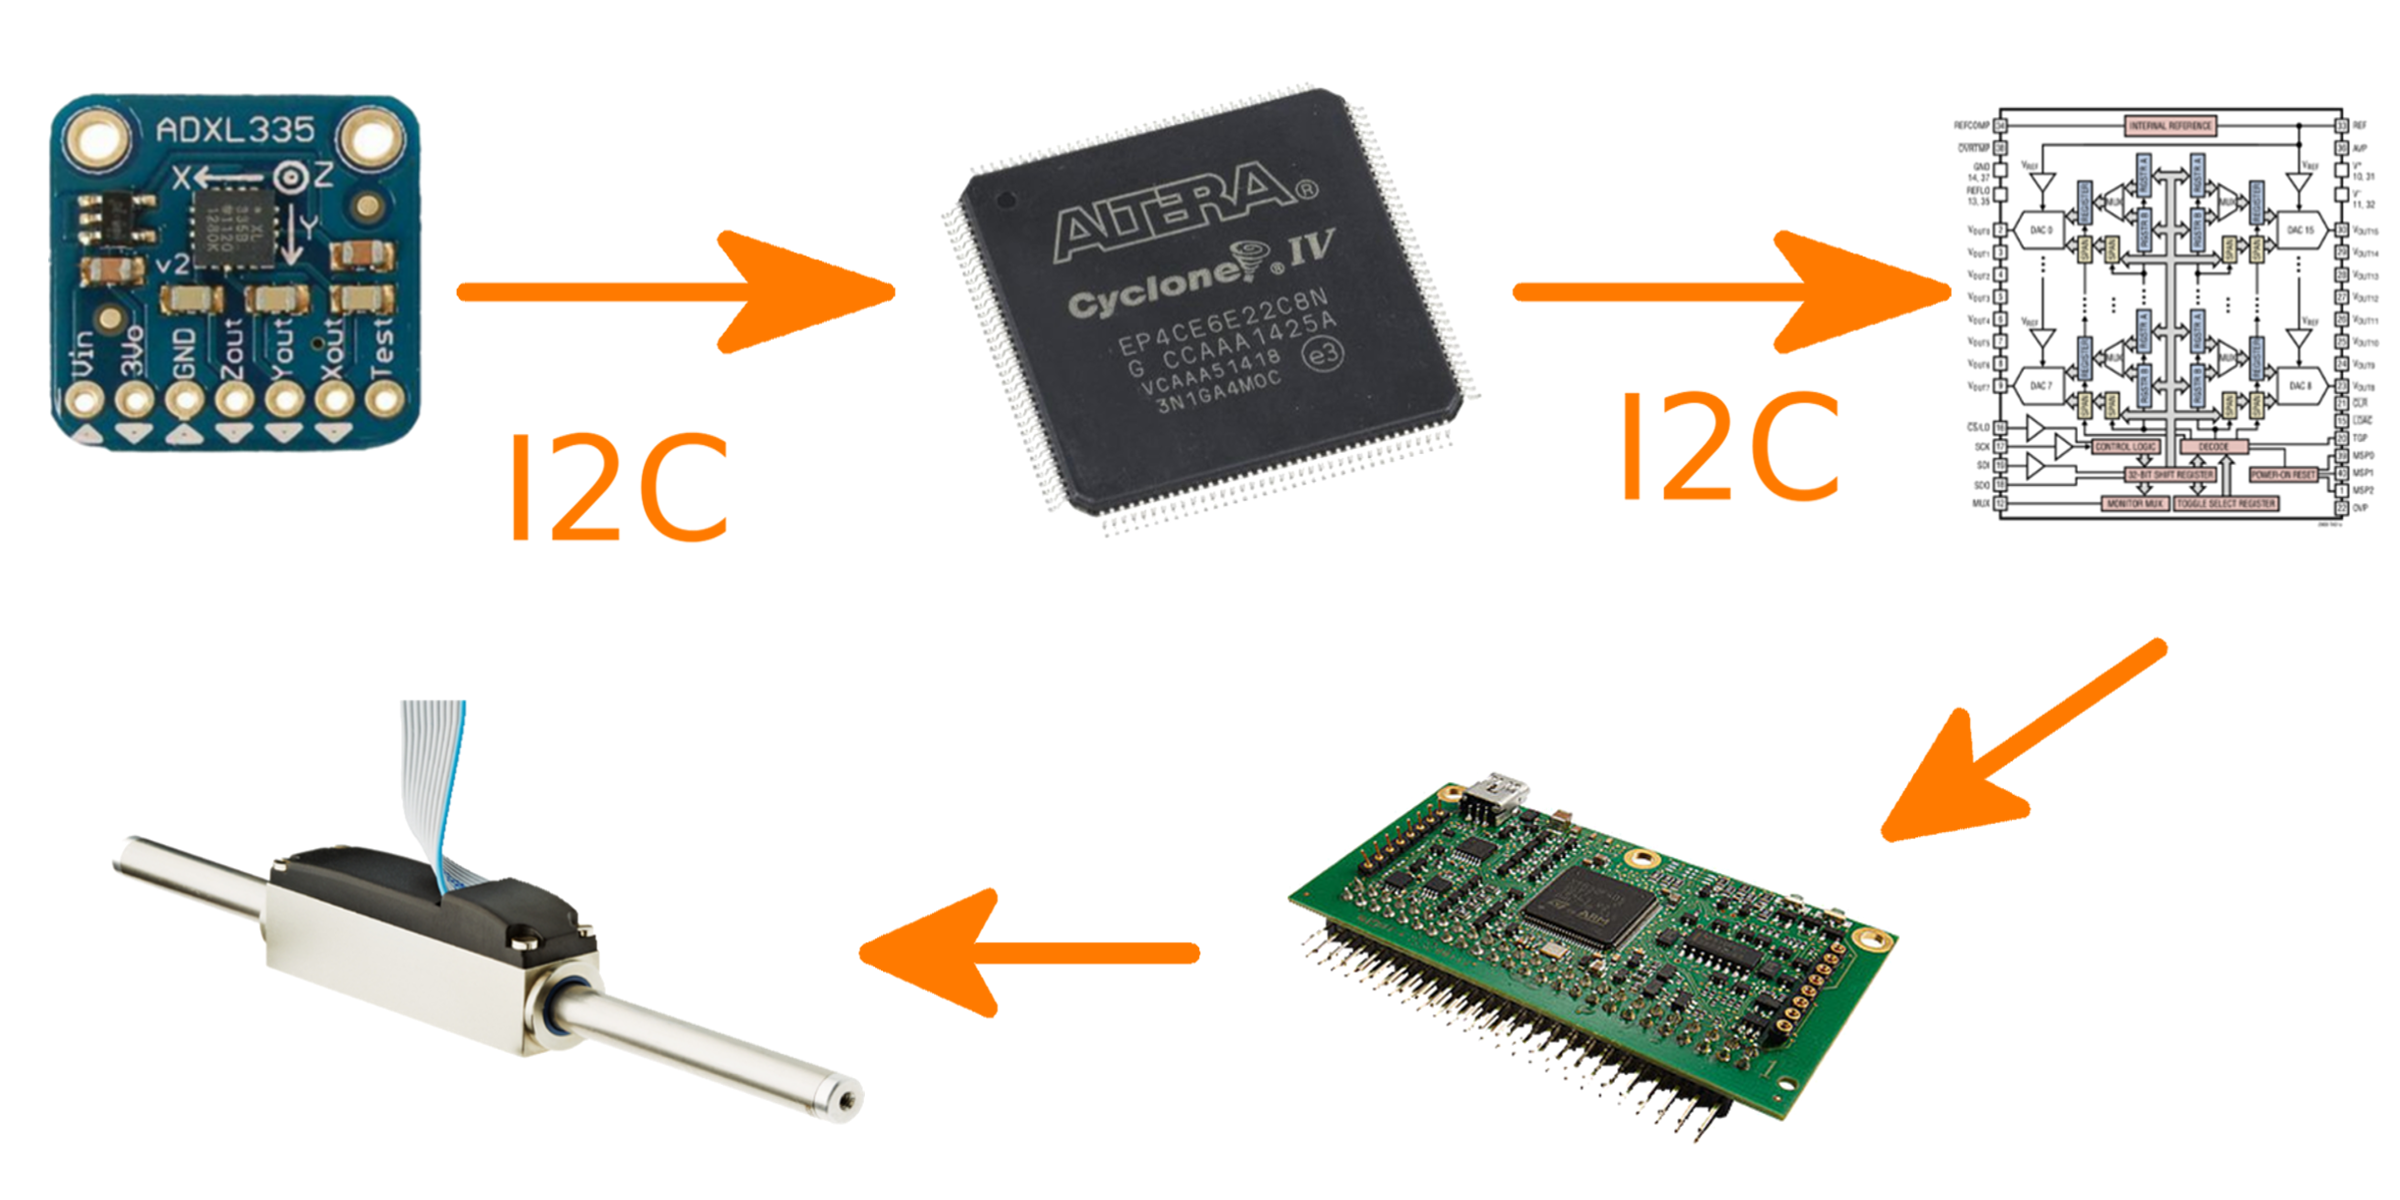
\includegraphics[width=17cm]{CH.png}\hss}\hfill\null
  	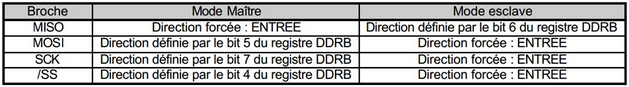
\includegraphics[width=14cm]{SPI2.png}
    \caption{SPI - signaux logiques}
	\end{figure}	
 
	\begin{itemize}
	\item SCLK (Serial Clock): Le signal d'horloge, il est utilisé pour synchroniser les données échangées entre le maître et 	les esclaves. Cette ligne est nécessairement une sortie sur le maître et une entrée sur le ou les esclaves.
 
	\item MOSI (Master Output, Slave Input): est utilisé pour transférer les données du maître vers l'esclave.
 
	\item MISO (Master Input, Slave Output): est utilisé pour transférer les données de l'esclave vers le maître.
 
	\item SS (Slave Select): le maître utilise ce signal pour choisir avec qui il veut dialoguer. Ce signal est actif à l'état bas. Les esclaves ne peuvent pas communiquer entre eux. Seul le maître peut autoriser un esclave à dialoguer, cela dit l'esclave ne peut commencer le dialogue que s'il n'a pas l'autorisation.
\end{itemize}
 
	On parlera aussi de liaison à trois fils : permet de véhiculer l’information dans les deux sens (bidirectionnelle), un fil différent étant dévolu à chaque sens de transfert d’information. Comme ceci permet la communication simultanée dans les deux sens de transmission, on parlera de liaison full-duplex : pendant que le maître transmet des données sur la ligne MOSI, vers l’esclave sélectionné, il en reçoit de celui-ci par la ligne MISO.

  		\subsubsection{Principe de transmission}
  		
			Une transmission SPI typique est une communication simultanée entre un maître et un esclave :
Tout d'abord, le maître initie la communication en sélectionnant l'esclave avec qui il veut communiquer par l'utilisation du signal SS qui est actif bas.
Ensuite, le maître et l'esclave préparent les données à envoyer dans leurs registres à décalage.
Enfin, le maître génère des impulsions d'horloge pour synchroniser les données échangées.
 
À chaque coup d'horloge, le maître et l'esclave s'échangent un bit. Après huit coups d'horloge le maître a transmis un octet à l'esclave et vice versa. La vitesse de l'horloge est réglée selon des caractéristiques propres aux périphériques.

	\begin{figure}[!ht]
    \center
    %\hfill\hbox to 0pt{\hss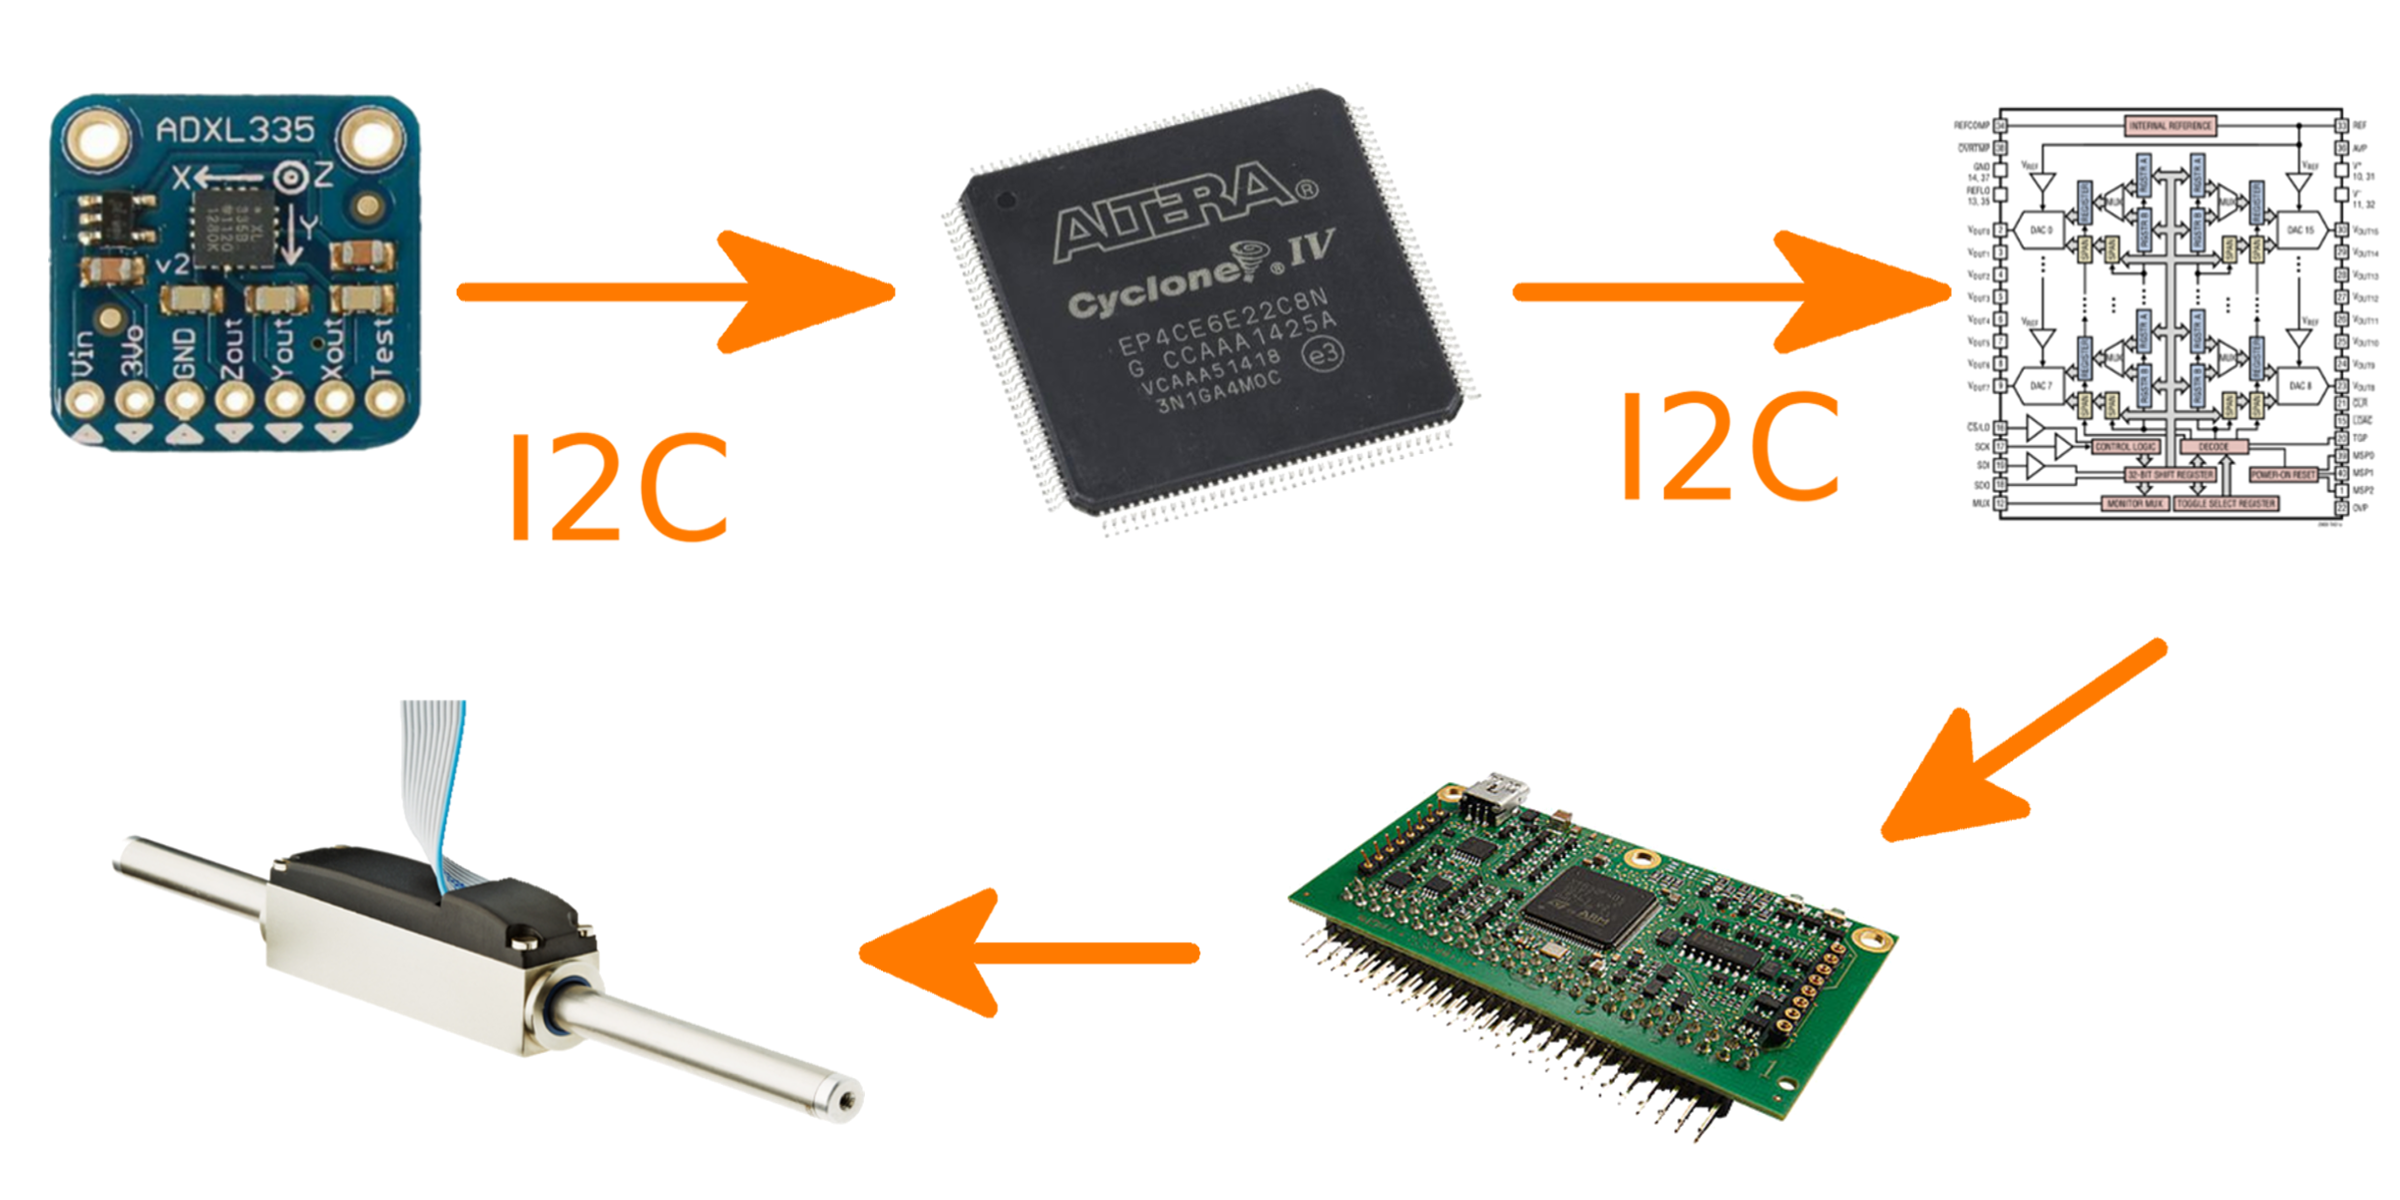
\includegraphics[width=17cm]{CH.png}\hss}\hfill\null
  	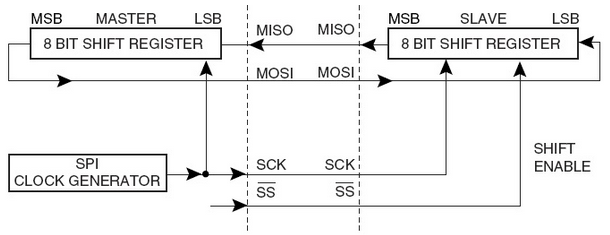
\includegraphics[width=10cm]{SPI3.png}
    \caption{SPI - shift register 1}
	\end{figure}
 
Pendant que le maître transmet les données sur la ligne MOSI, vers l’esclave sélectionné, il en reçoit de celui-ci par la ligne MISO.
Voici le tout sous forme de dessin. En rouge les bits reçus, en bleu les bits envoyés :

	\begin{figure}[!ht]
    \center
    %\hfill\hbox to 0pt{\hss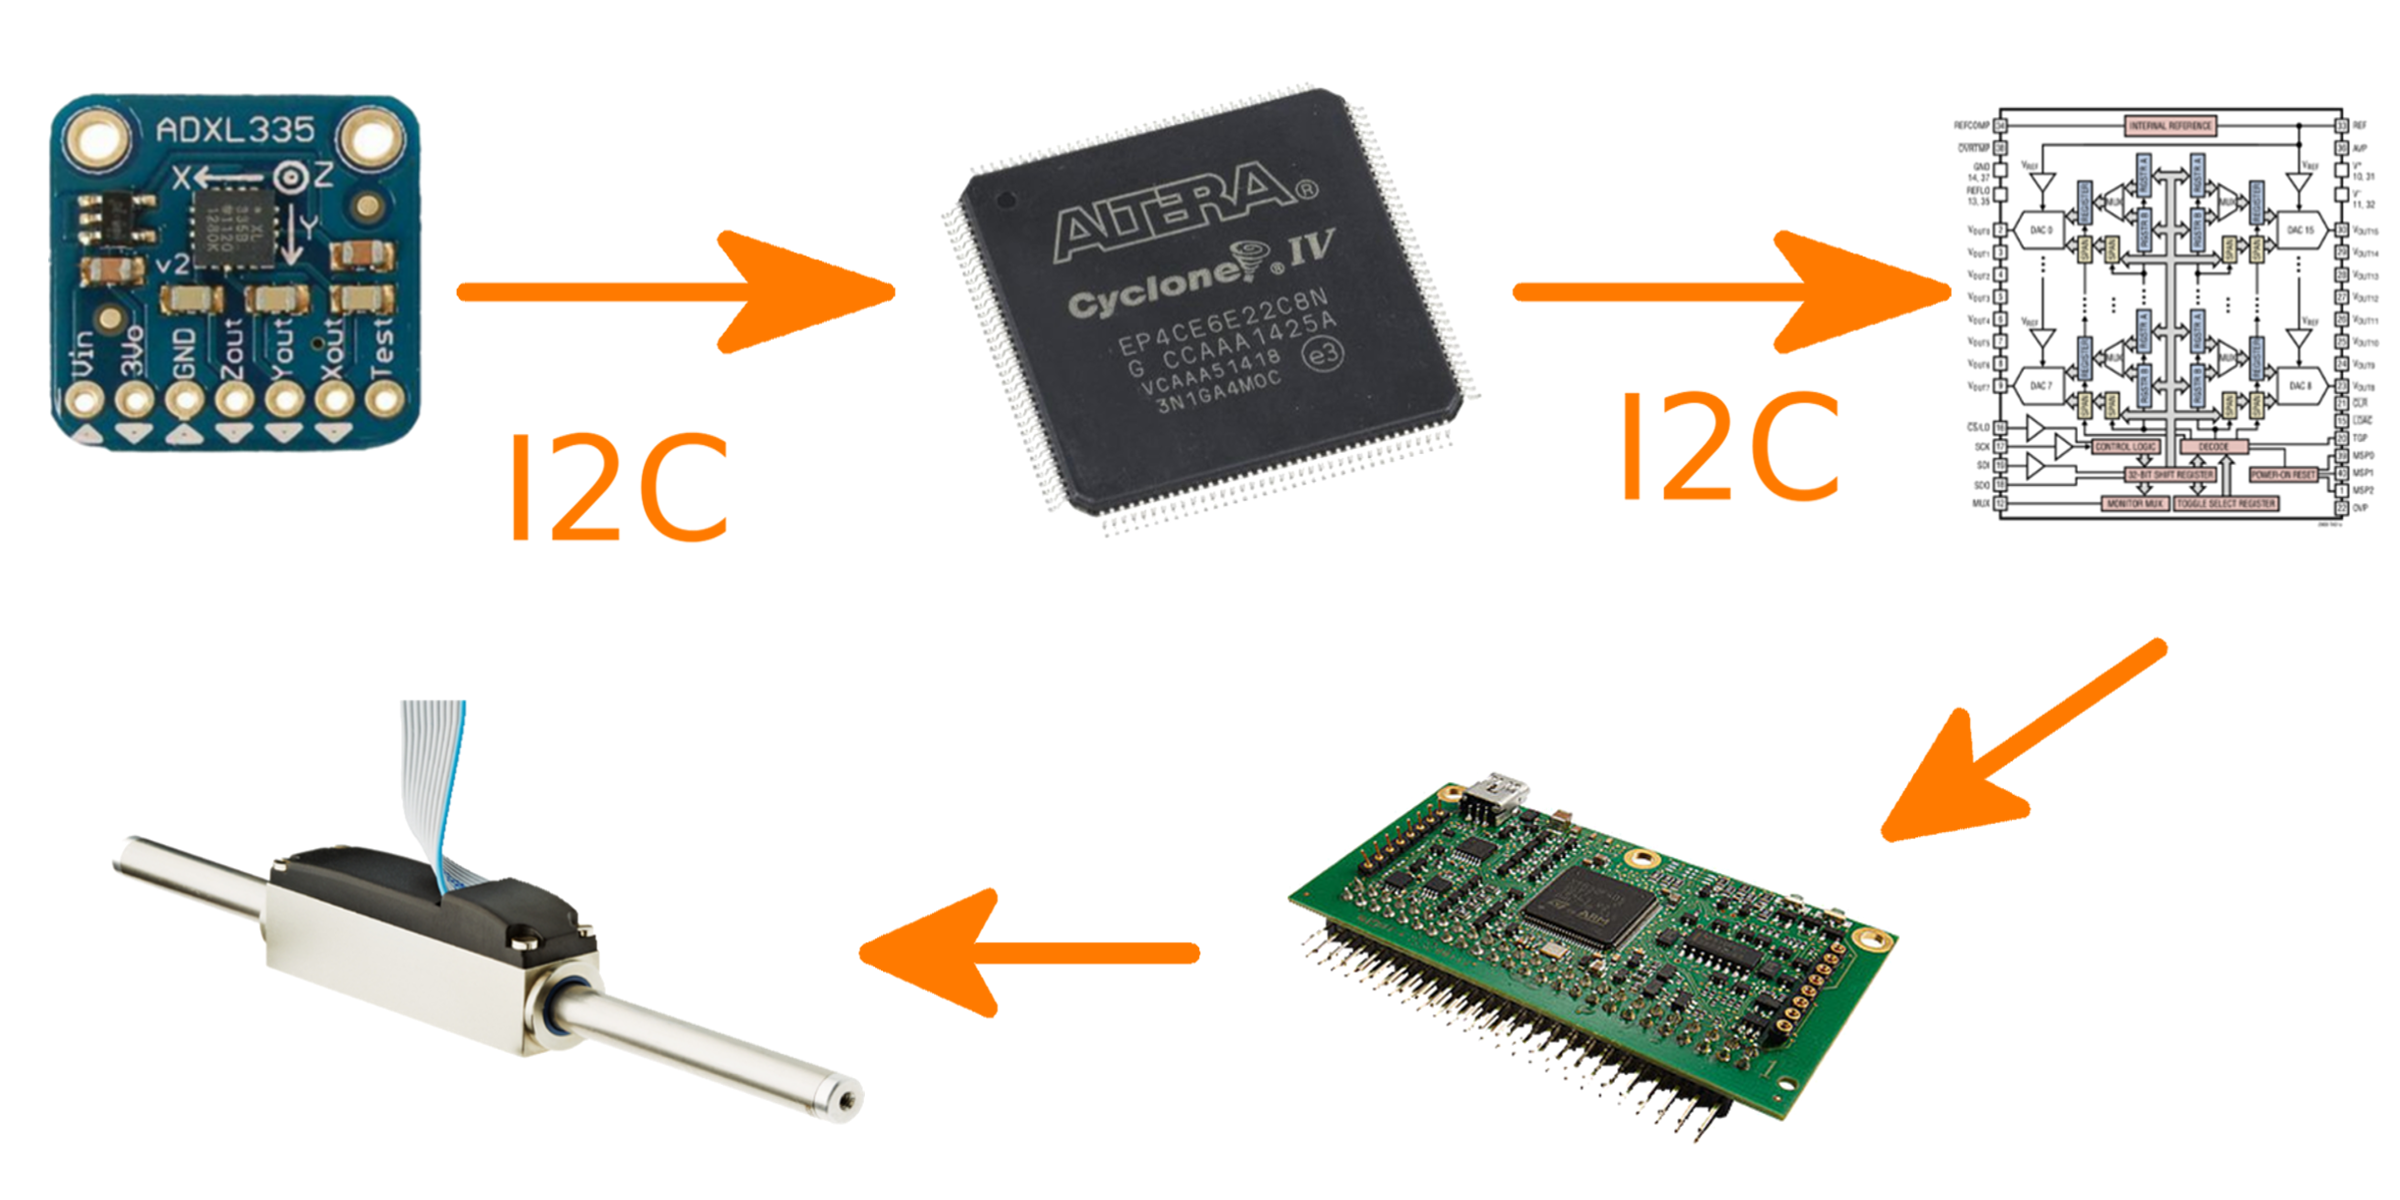
\includegraphics[width=17cm]{CH.png}\hss}\hfill\null
  	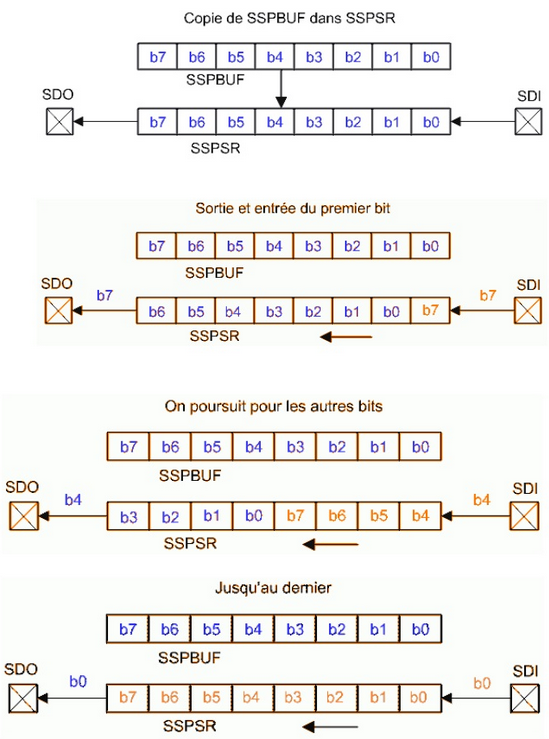
\includegraphics[width=7cm]{SPI4.png}
    \caption{SPI - shift register 2}
	\end{figure}
 
  		\subsubsection{Mode maître}
  		
  		Lorsqu'il est configuré en tant que maître, l'interface SPI n'a aucun contrôle automatique de la ligne de SS. Pour la configuration en mode maître, nous devons déclarer : MOSI, SS et SCLK en sortie ; MISO en entrée ; mettre le bit MSTR à '1' dans le registre SPCR. La mise de SS à l’état bas permet d'établir la communication avec l’esclave.
Le principe de transmission suit cet ordre :
 
    Ecriture d’un octet dans le registre de données (SPDR).
    Génération du signal d'horloge.
    Envoi des données contenues dans le registre de données vers l’esclave via la ligne MOSI.
    Arrêt du signal d'horloge.
    Mise du bit SPIF = 1 (flag de fin de communication)
    Si SPIE = 1 (autorisation de l’interruption) : interruption demandée, 2 options :
        chargement de l’octet suivant dans le registre
        mise de SS à l’état haut pour signaler la fin du paquet de données
 
	Le dernier octet entrant sera conservé dans le registre tampon pour une utilisation ultérieure.
 
  		\subsubsection{Mode esclave}
  		
  		Pour la configuration en mode esclave, nous devons déclarer : MOSI, SS et SCLK en entrée ; MISO en sortie ; Mettre le bit MSTR à '0' dans le registre SPCR. L’esclave reste en mode sommeil jusqu’à ce que le maître l'appelle (en mettant la ligne SS à l’état bas). La mise de SS à l’état bas permet d'établir la communication avec l’esclave. Le principe de transmission suit cet ordre :
 
    Sélection de l'esclave avec qui communiquer
    Génération du signal d'horloge par le maître
    Envoi des données contenues dans le registre des données vers l’esclave via la ligne MISO.
    Mise du bit SPIF = 1 (flag de fin de communication)
    Si SPIE = 1 (autorisation de l’interruption) :
        interruption demandée
        chargement de l’octet suivant dans le registre

			\subsubsection{Avantages}
 
			\begin{itemize}
			\item Communication full-duplex.
			\item Vitesse assez importante par rapport à l’I2C (10-100MBits/s).
			\item Partage d’un bus commun pour l’horloge, MISO et MOSI entre les périphériques.
			\item Simplicité de l’interface matérielle.
			\item Aucun arbitre nécessaire car aucune collision possible.
			\item Les esclaves utilisent l’horloge du maître et n’ont donc pas besoin d’oscillateur de précision.
			\end{itemize}
 
  		\subsubsection{inconvénients}
 
			\begin{itemize}
			\item Utilise plus de pattes d’un boitier que l’I2C qui en utilise seulement 2 (et la masse).
			\item Aucun adressage possible : il faut une ligne de sélection par esclave en mode non chaîné.
			\item Le protocole n’a pas d’acquittement. Le maître peut parler dans le vide sans le savoir.
			\item Il ne peut y avoir qu’un seul maître sur le bus.
			\item Ne s’utilise que sur de courtes distances contrairement aux liaisons RS-232, RS-485 ou bus CAN.
			\end{itemize}
 
 
 			\subsection{Bus I2C}
 			
 			Le bus I2C permet de faire communiquer entre eux des composants électroniques très divers grâce à seulement trois fils : un signal de données (SDA), un signal d'horloge (SCL), et un signal de référence électrique (masse).
Il s'agit d'une liaison en mode série synchrone (un bit est transmis à chaque coup d’horloge). Le nombre de composants qu'il est ainsi possible de relier est essentiellement limité par la charge capacitive des lignes SDA et SCL : 400 pF.
Un circuit maître et un ou plusieurs circuits esclaves peuvent être connectés au bus. Les échanges se font toujours à l’initiative du maître. La transmission est half duplex : mode écriture ou mode lecture, pas possible de manière simultanée.
 
  		\subsubsection{Connexion électrique}
  		
  		Tel qu'indiqué précédemment, pour se connecter à un bus I2C, il faut une masse et deux fils de communication. Le premier fil, SDA (Signal Data), est utilisé pour transmettre les données. L'autre fil, SCL (Signal CLock) est utilisé pour transmettre un signal d'horloge synchrone (signal qui indique le rythme d'évolution de la ligne SDA). Les tensions associées aux niveaux logiques vont dépendre de la technologie des circuits en présence (CMOS, TTL). Il faudra que tous les circuits connectés au bus I2C utilisent les mêmes potentiels pour définir les niveaux hauts et bas. En définitive, cela implique que tous les composants connectés à un même bus soient alimentés de façon identique.
  		
  \begin{figure}[!ht]
    \center
    %\hfill\hbox to 0pt{\hss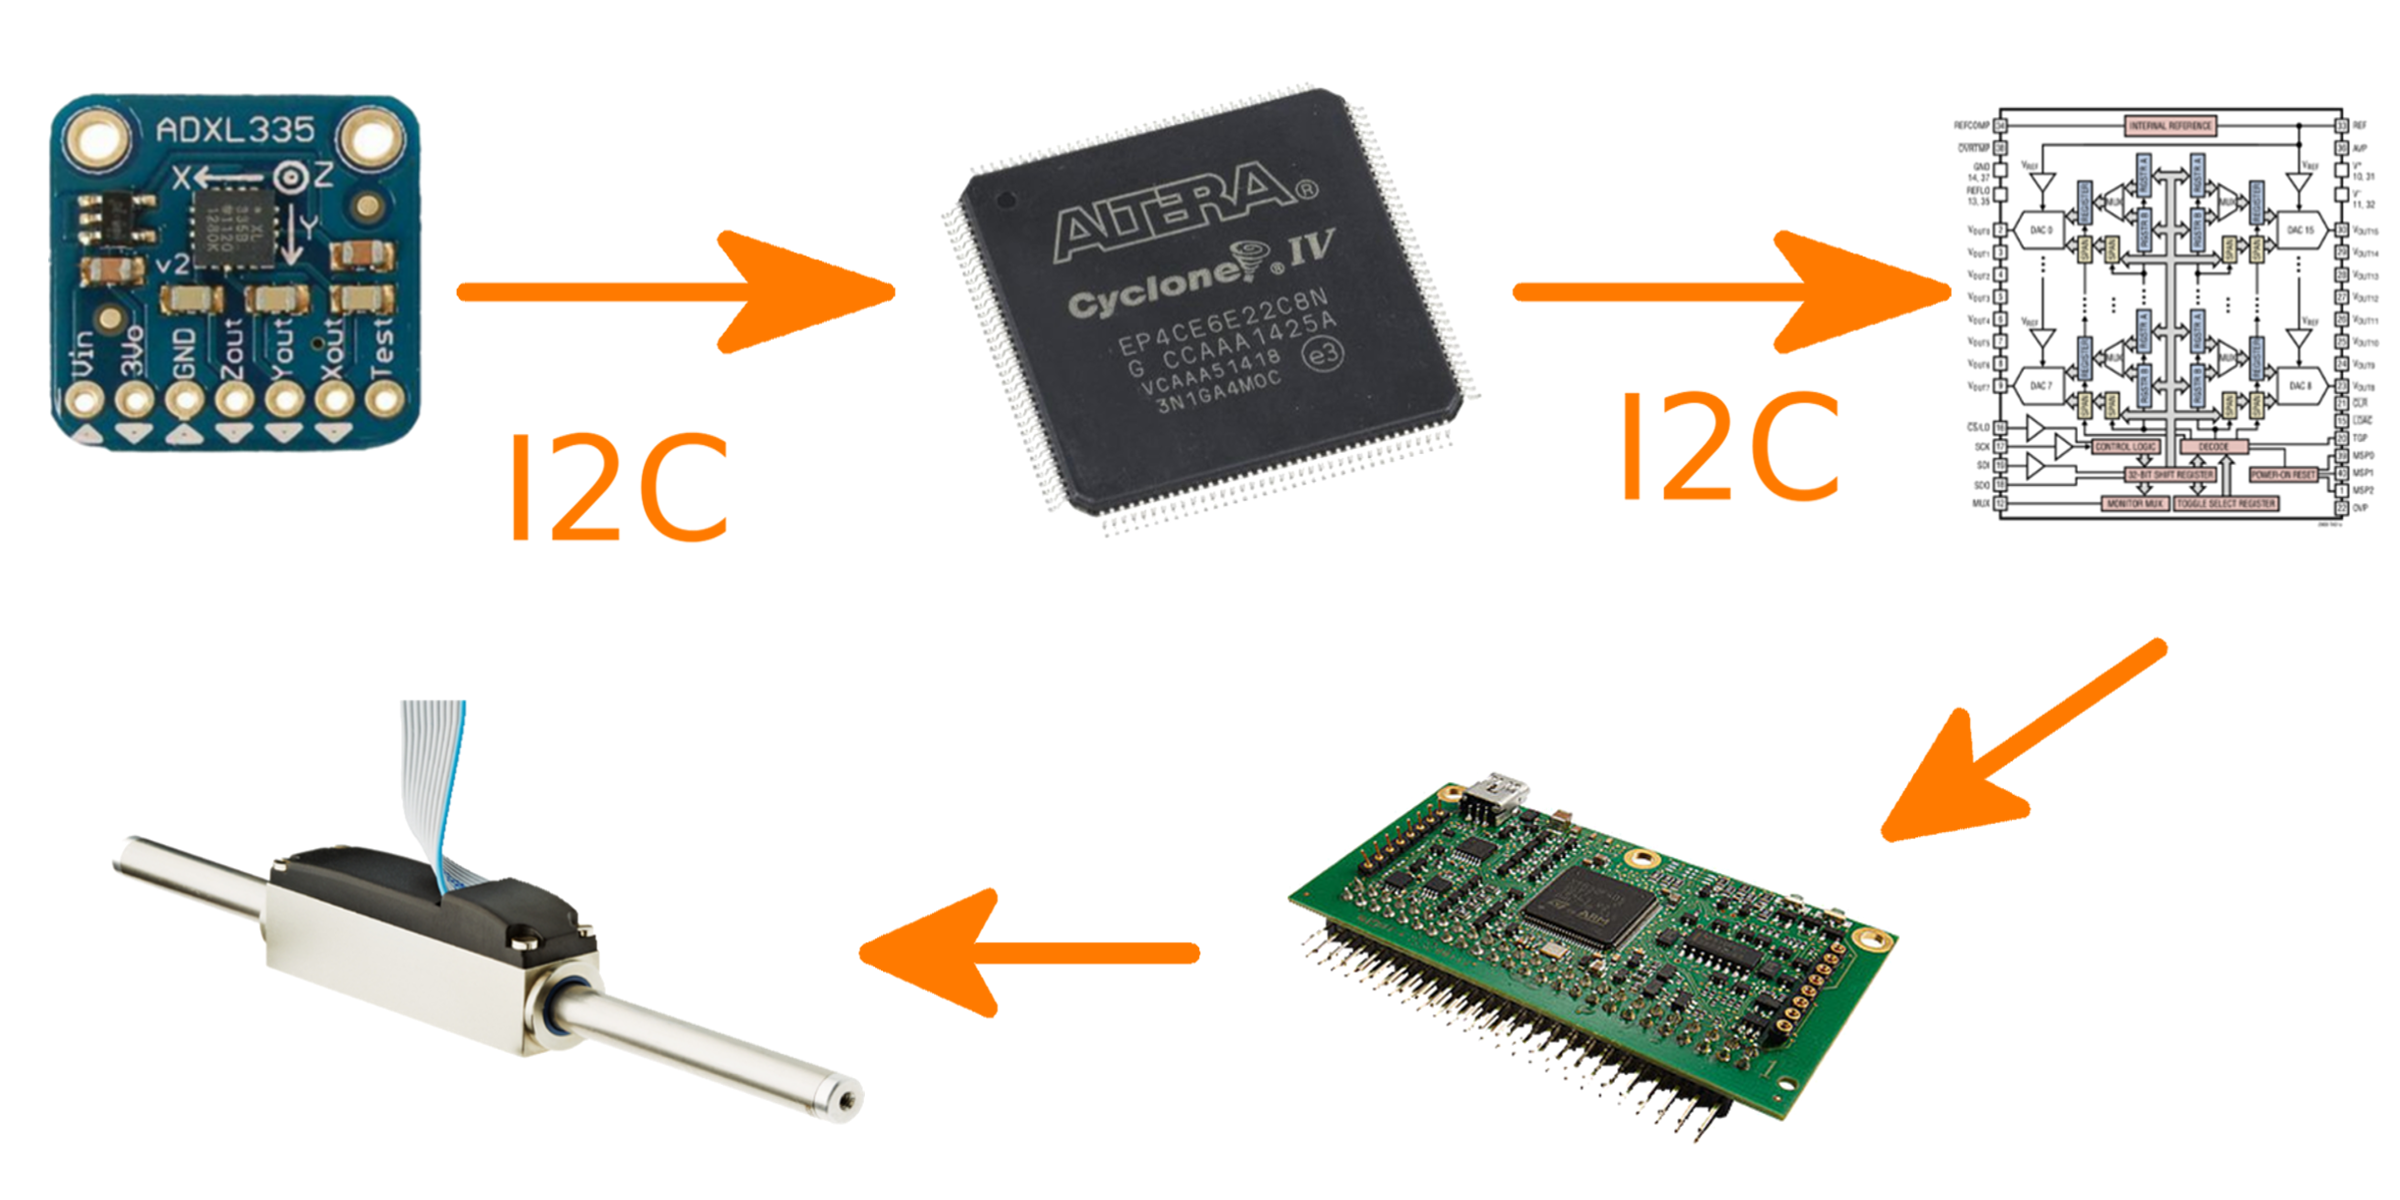
\includegraphics[width=17cm]{CH.png}\hss}\hfill\null
  	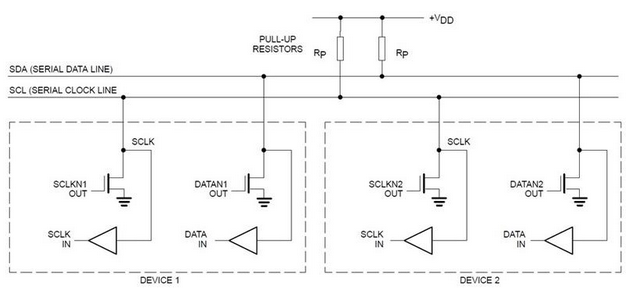
\includegraphics[width=12cm]{SPI5.png}
    \caption{SPI - electronique implémentation}
	\end{figure}
 
En ce qui concerne la lecture des signaux SDA et SCL, cela ne pose pas de problème. Les signaux peuvent être lus en permanence sans risque d'interférer sur le niveau de la ligne.
Au repos, tous les circuits connectés doivent imposer un niveau haut sur leurs sorties respectives. Si les lignes SDA et SCL sont au niveau haut dans ces conditions, cela signifie qu'aucun circuit ne tente de prendre le contrôle du bus. Si une des lignes SDA ou SCL passe à un niveau bas dans les mêmes conditions, c'est qu'un des circuits désire prendre le contrôle du bus. Mais il peut aussi y avoir deux circuits qui tentent de prendre le contrôle du bus en même temps (ou à quelques nanosecondes d'écart près). Il faut donc mettre en place un protocole pour gérer les conflits possibles.

   		\subsubsection{Protocole I2C}
	Le protocole I2C présente différentes caractéristiques:
 
			\begin{itemize}
			\item Maître-esclaves, car seul un nœud maître peut communiquer avec les esclaves du réseau (1 ou tous)
			\item Multi-maître, car plusieurs maîtres peuvent être présents sur le réseau
			\item Synchrone, car on utilise un mécanisme de requête/réponse
			\item Half-duplex, car on peut communiquer dans les deux sens, mais pas simultanément
			\end{itemize}
 
On utilise un adressage sur sept bits pour identifier les nœuds, ce qui permet (en théorie) jusqu’à 128 nœuds sur le réseau. Certaines adresses sont réservées pour le broadcast (communiquer vers tous les nœuds en même temps). En pratique, les constructeurs ont tendance à fixer l’adresse de certains nœuds, ce qui peut causer des collisions.
 
 
  		\subsubsection{Avantages}
			\begin{itemize}
			\item Utilise seulement deux lignes (+ le fil de masse) et simplicité de connexion (uniquement deux résistances de pull-up à rajouter) 
			\item Le protocole limite automatiquement la vitesse de transmission à la vitesse de l’élément le plus lent. 
			\item Le bit de reconnaissance qui permet de savoir si l’esclave est bien connecté et également si les données ont été correctement transmises ou non. 
			\item Interconnections de multiples périphériques
			\end{itemize}
 
  		\subsubsection{Inconvénients}
			\begin{itemize}
			\item Impossibilité d’utiliser un mode full-duplex 
			\item Vitesse relativement lente pour la plupart des périphériques esclaves (100 à 400kbits/s) 
			\item Consommation relativement élevée due à la configuration en collecteur/drain ouvert 
			\item Distance de communication limitée car les lignes du bus ne sont pas protégées des perturbations et envoient des fronts montant et descendant. Cette distance est donc limitée par la vitesse de communication, les résistances de pull-up, la capacité du bus (en général, autour des 400pF).
\end{itemize}
 
 \subsection{Contrainte et choix de réalisation}
Concernant les contraintes techniques auxquelles nous avions à faire face, nous retrouvons, une vitesse d'échange de données relativement importante (supérieur à 1 Mega), une simplicité vis-à-vis de l'interface matérielle afin de minimiser le nombre de fils utilisés, un bus stable sans interférence et enfin une distance de communication assez longue.

Au final, bien que de base, le bus I2C n'implique l'utilisation que de deux fils de communication (contrairement au bus SPI en nécessitant plus), le bus SPI répond aux principaux critères de vitesse de communication et une distance de transmission élevée. De plus, ce choix est renforcé du fait que nous avons réussi à réaliser un "hack" sur le protocole SPI de notre accéléromètre afin de minimiser le nombre de fil, comme nous le verrons dans la prochaine partie.


\chapter{"Hack" du protocol SPI}
	Nous l'avons vu précédemment, le nombre de fils branchés entre notre accéléromètre et notre carte programmable (FPGA) est une contrainte que nous souhaitons minimiser le plus possible; ainsi, le choix du SPI, en plus des qualitées de ce bus de communication, fut renforcé car nous nous sommes aperçus qu'un détournement de la technologie était possible, afin de diminuer le nombre de fils.
	
	Dernièrement, nous avons vu que le bus SPI fonctionnait comme suivant, étant basé sur quatre éléments distincts de communication:
	
	\begin{itemize}
		\item SCLK (Serial Clock) 
		\item MOSI (Master Output, Slave Input) 
		\item MISO (Master Input, Slave Output) 
		\item SS (Slave Select)
	\end{itemize}
	
	Dans cette configuration, chacun de ces quatre canaux représente un fil de communication. Nous avons donc cherché à identifier quels canaux pouvaient être supprimés ou mutualisés. Concernant la "Clock" et le "Select Slave", la suppression d'un de ces canaux entraînerait la paralysation du protocole, et il en va de même pour une mutualisation; c'est donc vers les canaux de communication que nous nous sommes tournés.
	
	En effet, de deux fils de communication unidirectionnels, il serait intéressant de pouvoir les mutualiser afin d'offrir un canal de communication bidirectionnel. Cette observation est de plus renforcée, étant donné que notre contrôleur FPGA met à disposition des broches pouvant être utilisées simultanément en entrée ainsi qu'en sortie; au sein du langage VHDL, ce type de broche est défini comme suivant: "INOUT".
	
	Sachant maintenant que l'implémentation d'une broche bidirectionnelle est possible du côté de notre processeur, il nous faut déterminer si elle est également possible du côté de notre accéléromètre. Pour cela, avec un oscilloscope, nous allons chercher à déterminer si la ligne MISO ou la ligne MOSI "drive" la ligne au repos ou non.
	
	Afin de déterminer si oui ou non notre accéléromètre drive la ligne, nous avons mis en place une petite manipulation mettant en oeuvre un oscilloscope, une résistance, ainsi que notre accéléromètre. Nous avons utilisé notre résistance en tant que résistance de tirage à la masse (pull-down); ce montage nous permet d'appliquer un niveau "mou" à la ligne en externe, ainsi nous allons pouoir observer si la ligne diffère de la valeur par défaut.	
	
	À partir de là, deux situations étaient possibles: soit le niveau de la ligne se maintient à la valeur par défaut (apporté par le montage pull-down), soit le niveau de la ligne diffère de cette dernière; c'est alors que la ligne est drivée par un composant, rendant ainsi toute possibilité de mutualisation impossible.
	
	Suite à notre manipulation, nous avons pu mettre en évidence que notre accéléromètre ne "drive" pas la ligne, étant donné que cette derrière ne diffère pas de la valeur par défaut, nous permettant de mettre en place la mutualisation souhaitée des lignes MISO MOSI.
	
	Ayant pu adapter le protocole SPI de notre accéléromètre à nos besoins, afin d'en minimiser le nombre de fils, il nous est maintenant possible de nous concentrer sur la mise en place de la chaîne dans son ensemble.
	
	\chapter{De l'accéléromètre au FPGA}
	
		Afin de mettre en oeuvre un échange de données entre notre accéléromètre et notre carte programmable (FPGA), il nous a fallu mettre en place notre protocole de communication précédemment sélectionné, le bus SPI. Le protocole devant être impléménter au travers du langage VHDL, propre au circuit logique programmable.
		
		Mais disposant d'un temps limité par le stage, ainsi que par la volonté de mettre en place une chaîne de contrôle complète, et de plus, ayant au début du stage des connaissances limitées en VHDL ainsi que de la philosophie, de la façon de penser et de concevoir des programmes, qui est en tout point différent de la progammation logiciel sur micro-contrôleur, nous avons fait le choix de nous tourner vers un module "SPI MASTER" open-source.		
		Ce module "SPI MASTER" va s'intégrer pour travailler au plus près du matériel, afin de mettre en place une interface entre le comportement physique du SPI de notre accéléromètre et notre interface plus "haut niveau" au travers de laquelle nous exploitons le protocole SPI.
		
		"Ce module "SPI MASTER" permet une programmation flexible de composant logique, afin de mettre en place une communication avec divers esclaves au travers d'une interface parallèle. Il permet la communication avec un nombre d'esclaves à définir, pouvant être traités de manière indépendante, au travers du champ de données et de la fréquence de contrôle."
		
		\section{Contexte}
			Le schéma de la communication SPI revient à interface full-duplex (transport simultané de l'information dans les deux sens) utilisant quatre fils. L'horloge (SCLK) drivée par le maître, mettant à disposition une horloge synchrone. Ensuite, le maître transmet la donnée via la sortie "Master out, Slave In" (MOSI) et reçoit celle du capteur par la ligne "M	aster In, Slave Out" (MISO).
			
			Un maître peut communiquer avec un module esclave de diverse manière, mais la méthode commune revient à configurer chaque module esclave avec une ligne "Select Slave" indépendante et en partageant les autres lignes (horloge, miso, mosi) entre les différents modules esclaves. Grâce à cette méthode, un module va ignorer les lignes partagées, tant que les lignes "SS" ne seront pas activées (mises à l'état bas).
			
	\begin{figure}[!ht]
    \center
    %\hfill\hbox to 0pt{\hss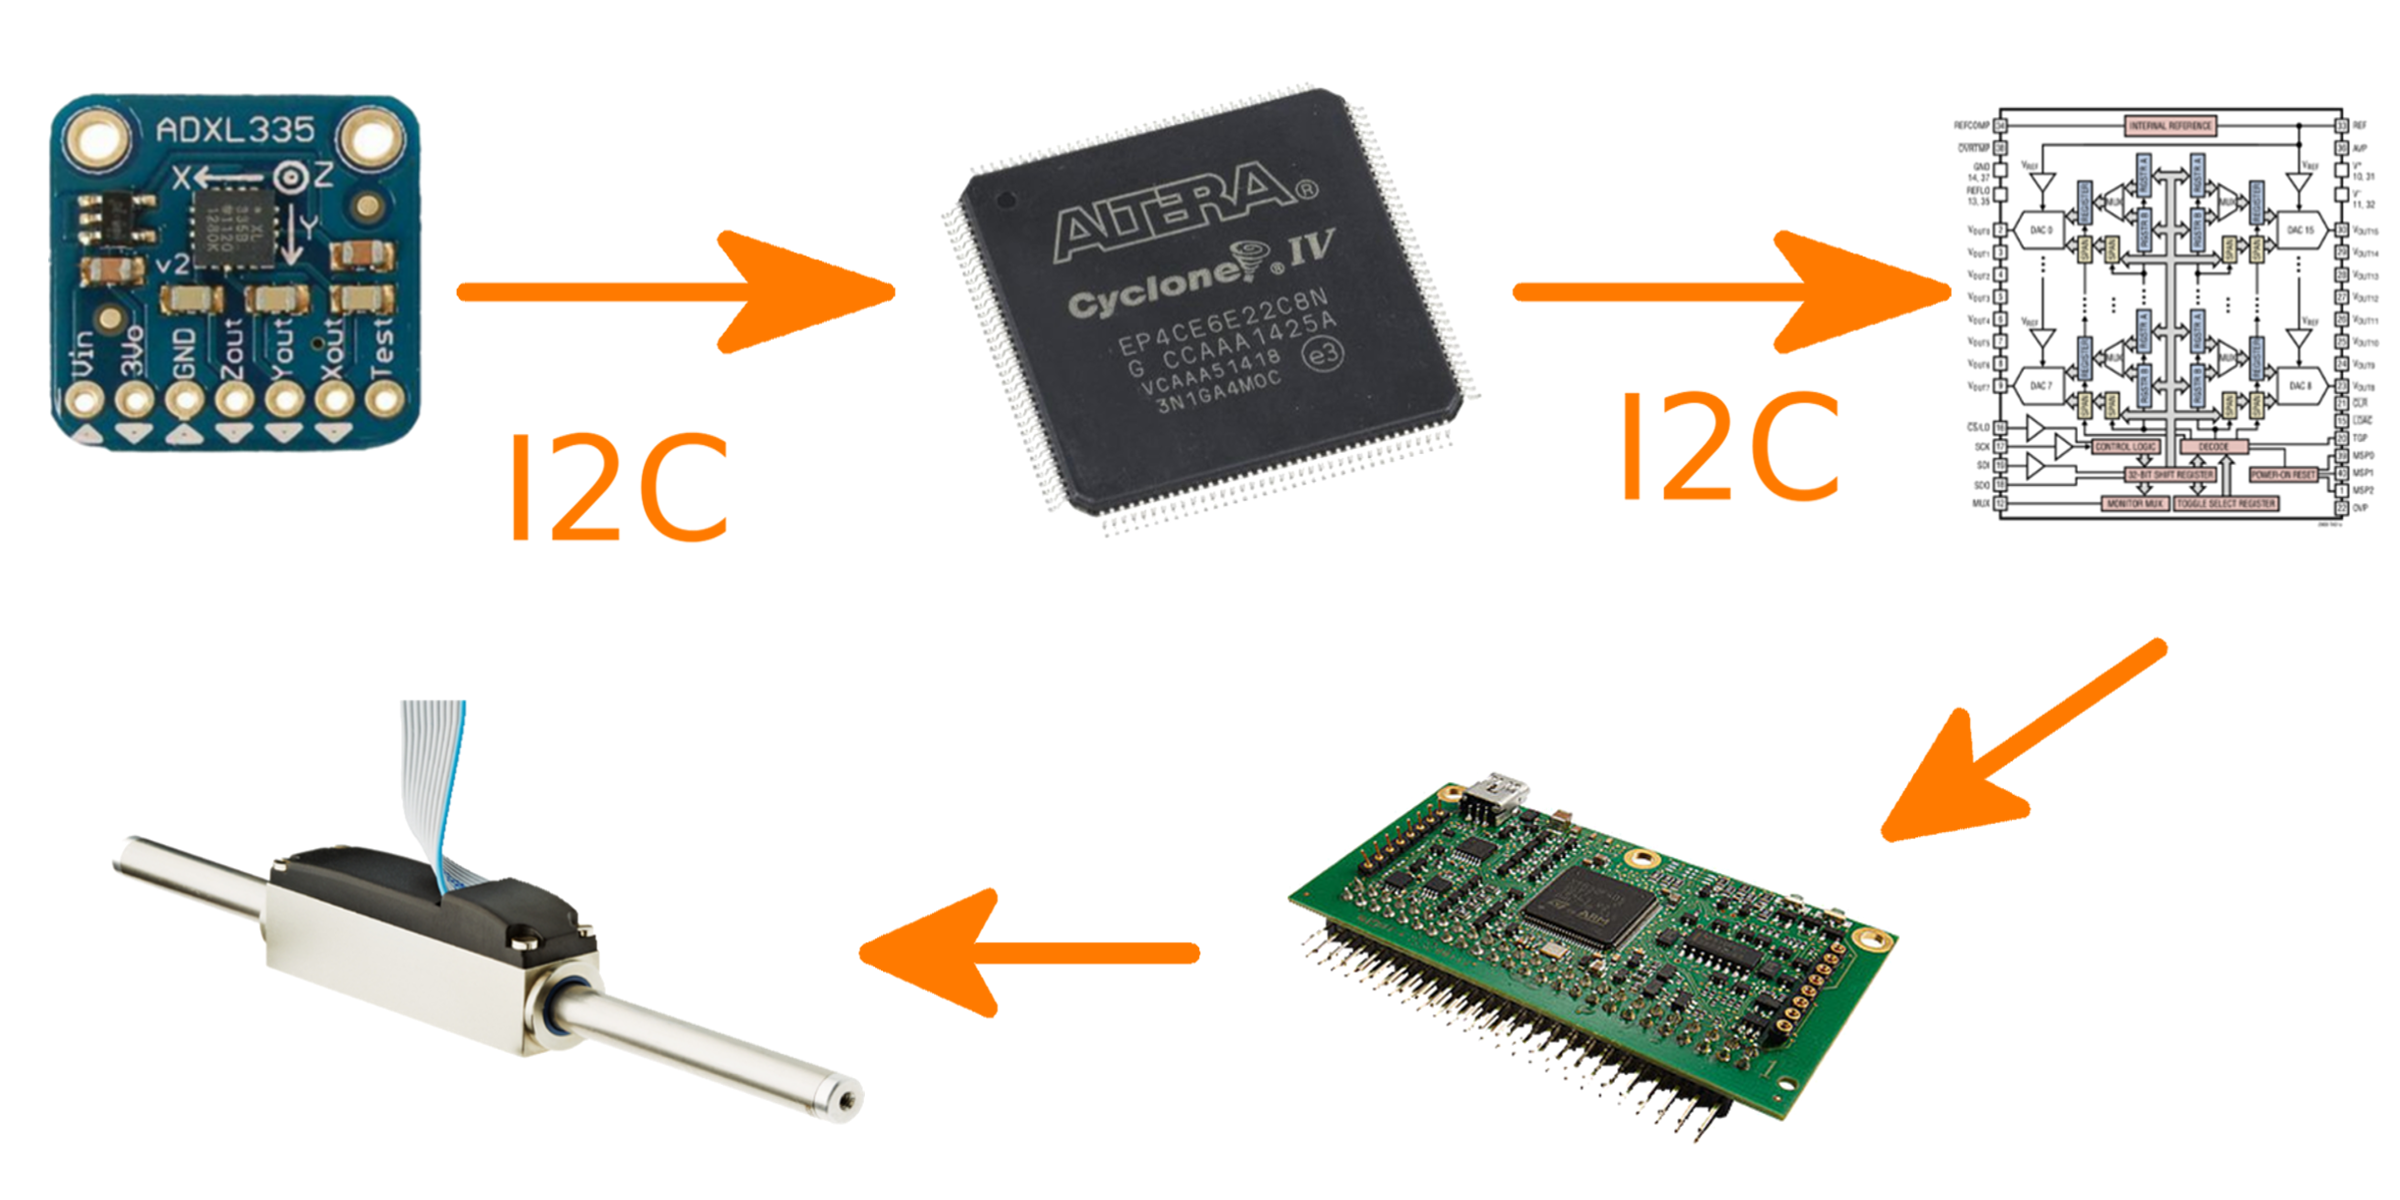
\includegraphics[width=17cm]{CH.png}\hss}\hfill\null
  	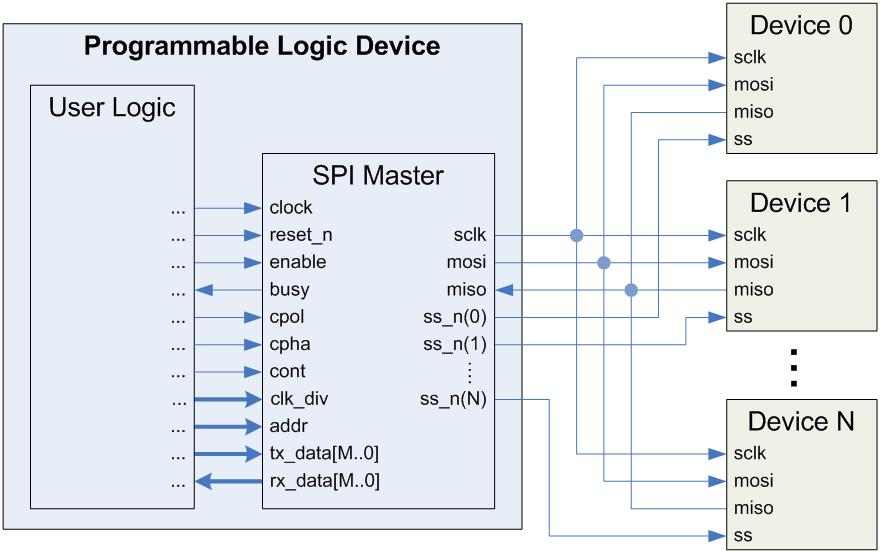
\includegraphics[width=10cm]{spi_master_block.JPG}
    \caption{SPI - implémentation commune}
	\end{figure}
	
	Le protocole SPI a quatre modes de déploiement, basés sur deux paramètres, clock polarity (CPOL) et clock phase (CPHA). Le maître et l'esclave doivent utiliser le même mode de communication. 
	Dans le cas ou CPOL serait à zéro, alors SCLK doit être à l'état haut, et le premier front de l'horloge serait un front montant.
	CPHA, lui, définit l'alignement des données, ainsi si CPHA est à zéro, alors le premier bit de données écrit, lors du front descendant de la ligne "SS" est lu lors du premier front de l'horloge. Si CPHA est à un, la donnée est écrite sur le premier front de l'horloge et lu sur le deuxième front.
	Toute la procédure décrite ci-dessus est décrite dans la figure suivante:
	
	\begin{figure}[!ht]
    \center
    %\hfill\hbox to 0pt{\hss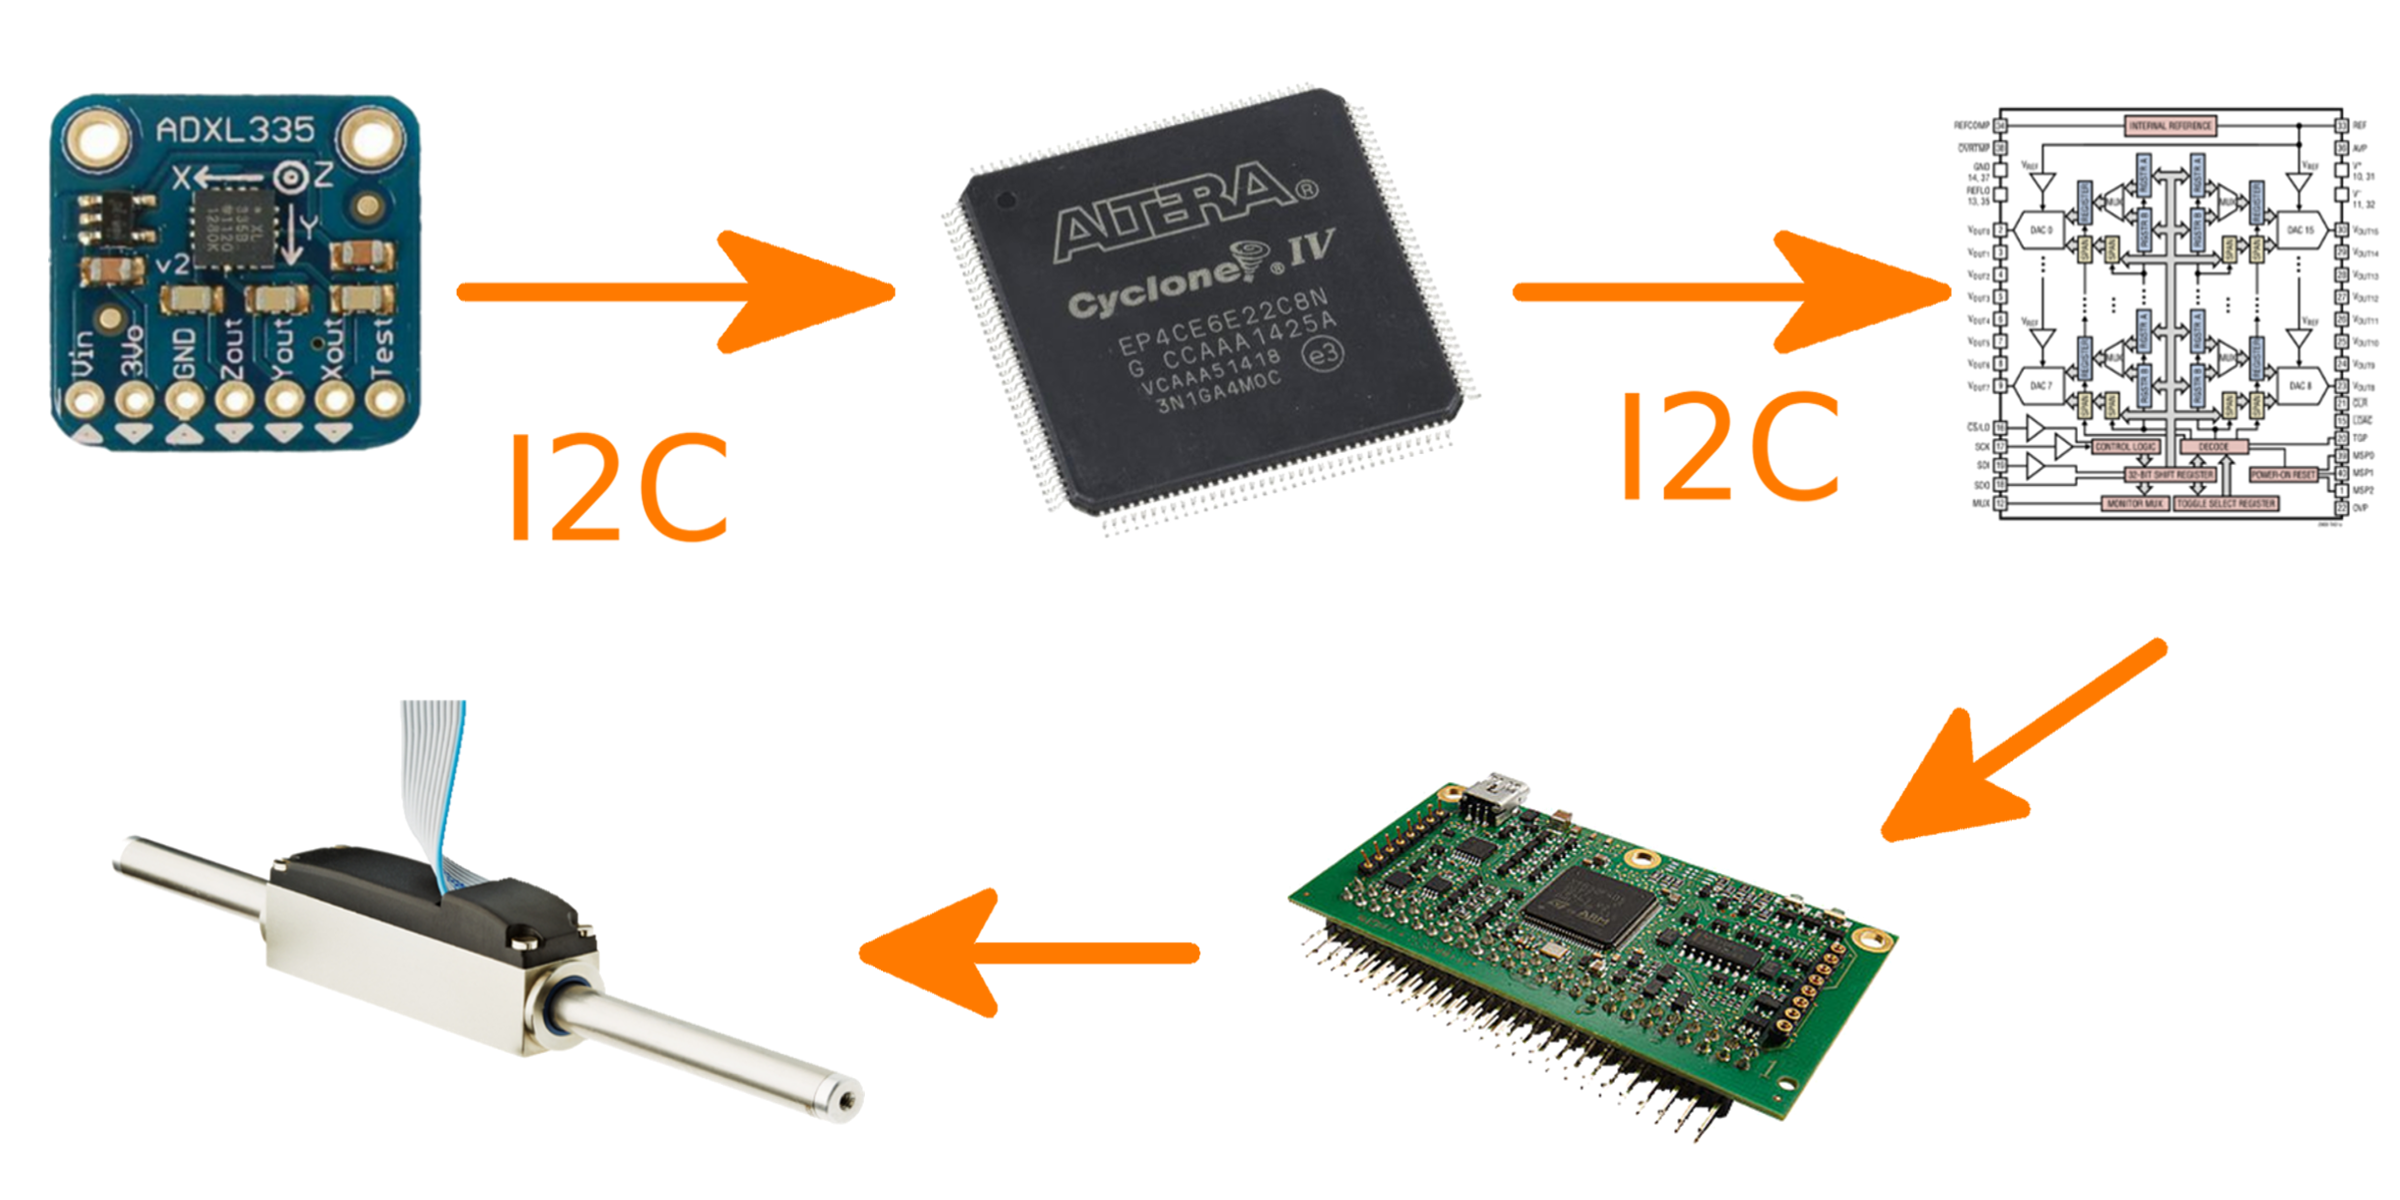
\includegraphics[width=17cm]{CH.png}\hss}\hfill\null
  	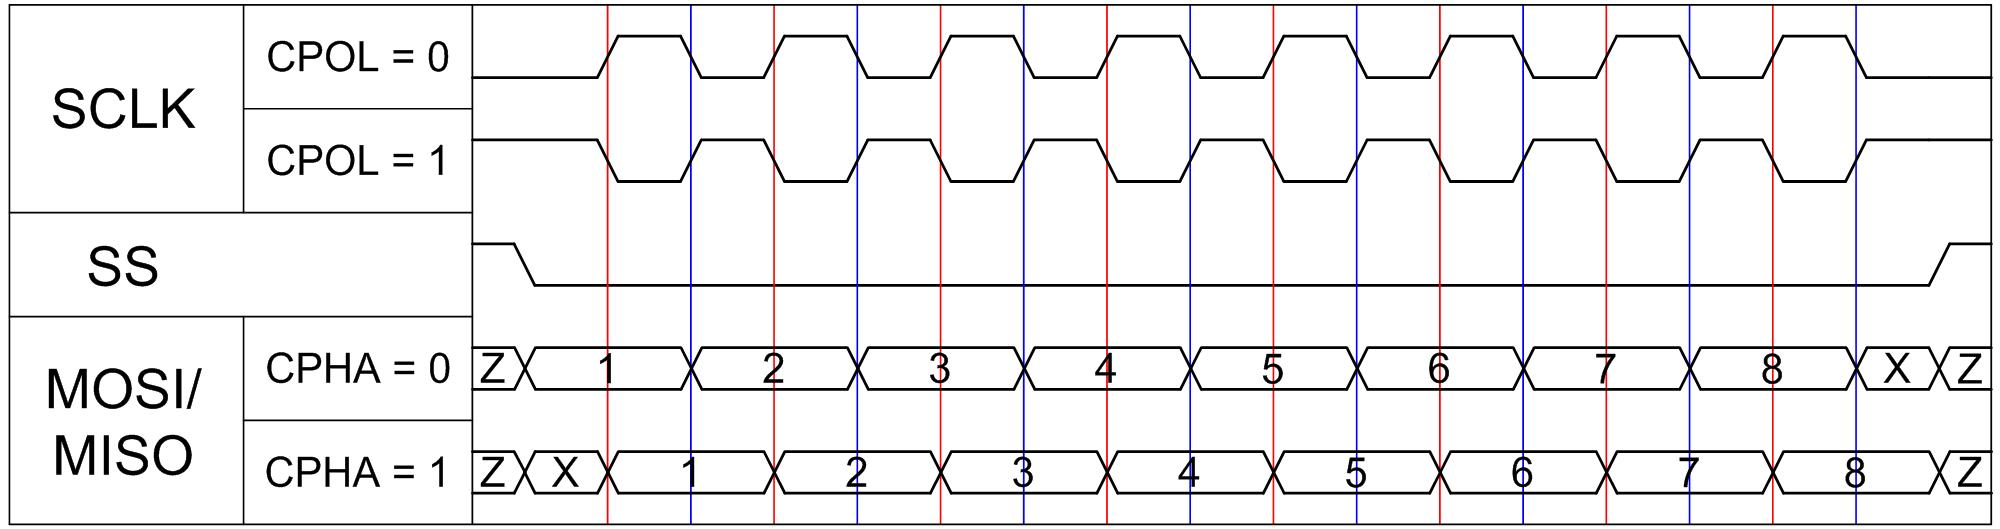
\includegraphics[width=12cm]{spi_timing_diagram.JPG}
    \caption{SPI - CPOL , CPHA}
	\end{figure}
	
	\section{Port utilisé}
		\begin{itemize}
			\item clock - Input - système clock
			\item reset\_n - Input - reset à l'état bas asynchrone
			\item enable - Input - loquet permettant d'initier une transaction
			\item CPOL - Input - SPI clock polarity
			\item CPHA - Input SPI clock phase
			\item clk\_div - Input - prescaler de la fréquence système
			\item Addr - Input - adresse de l'esclave ciblé
			\item Tx-data - Input - données à transmettre
			\item miso - Input
			\item mosi - Input
			\item sclk - inuput
			\item  ss\_n - input
			\item busy - out - signal pour la lecture des données
			\item rx-data - out - Données reçues de l'esclave.
		\end{itemize}
	
	\section{transaction}
		Un état sur le port "busy" indique que le composant est prêt à accepter une commande. Le composant verrouille les paramètres (adresse et données) pour la transmission sur le premier front montant de l'horloge, lorsque le port "enable" sera confirmé. Ensuite, sur la clock suivante, le composant configure le signal "busy" et commence la transaction. Une fois complète, ce dernier reçoit les données sur le port "rx\_data" et ce bit de données reste sur le port jusqu'à l'arrivée du projet, généralisant ce fonctionnement tant que la transaction ne sera pas terminée.		
		
		La figure suivante illustre une transaction typique. Le module maître transmet la donnée "1001" au module esclave, configuré avec CPOL = 1 et CPHA = 1, le maître reçoit en retour la donnée "1010".
		
	\begin{figure}[!ht]
    \center
    %\hfill\hbox to 0pt{\hss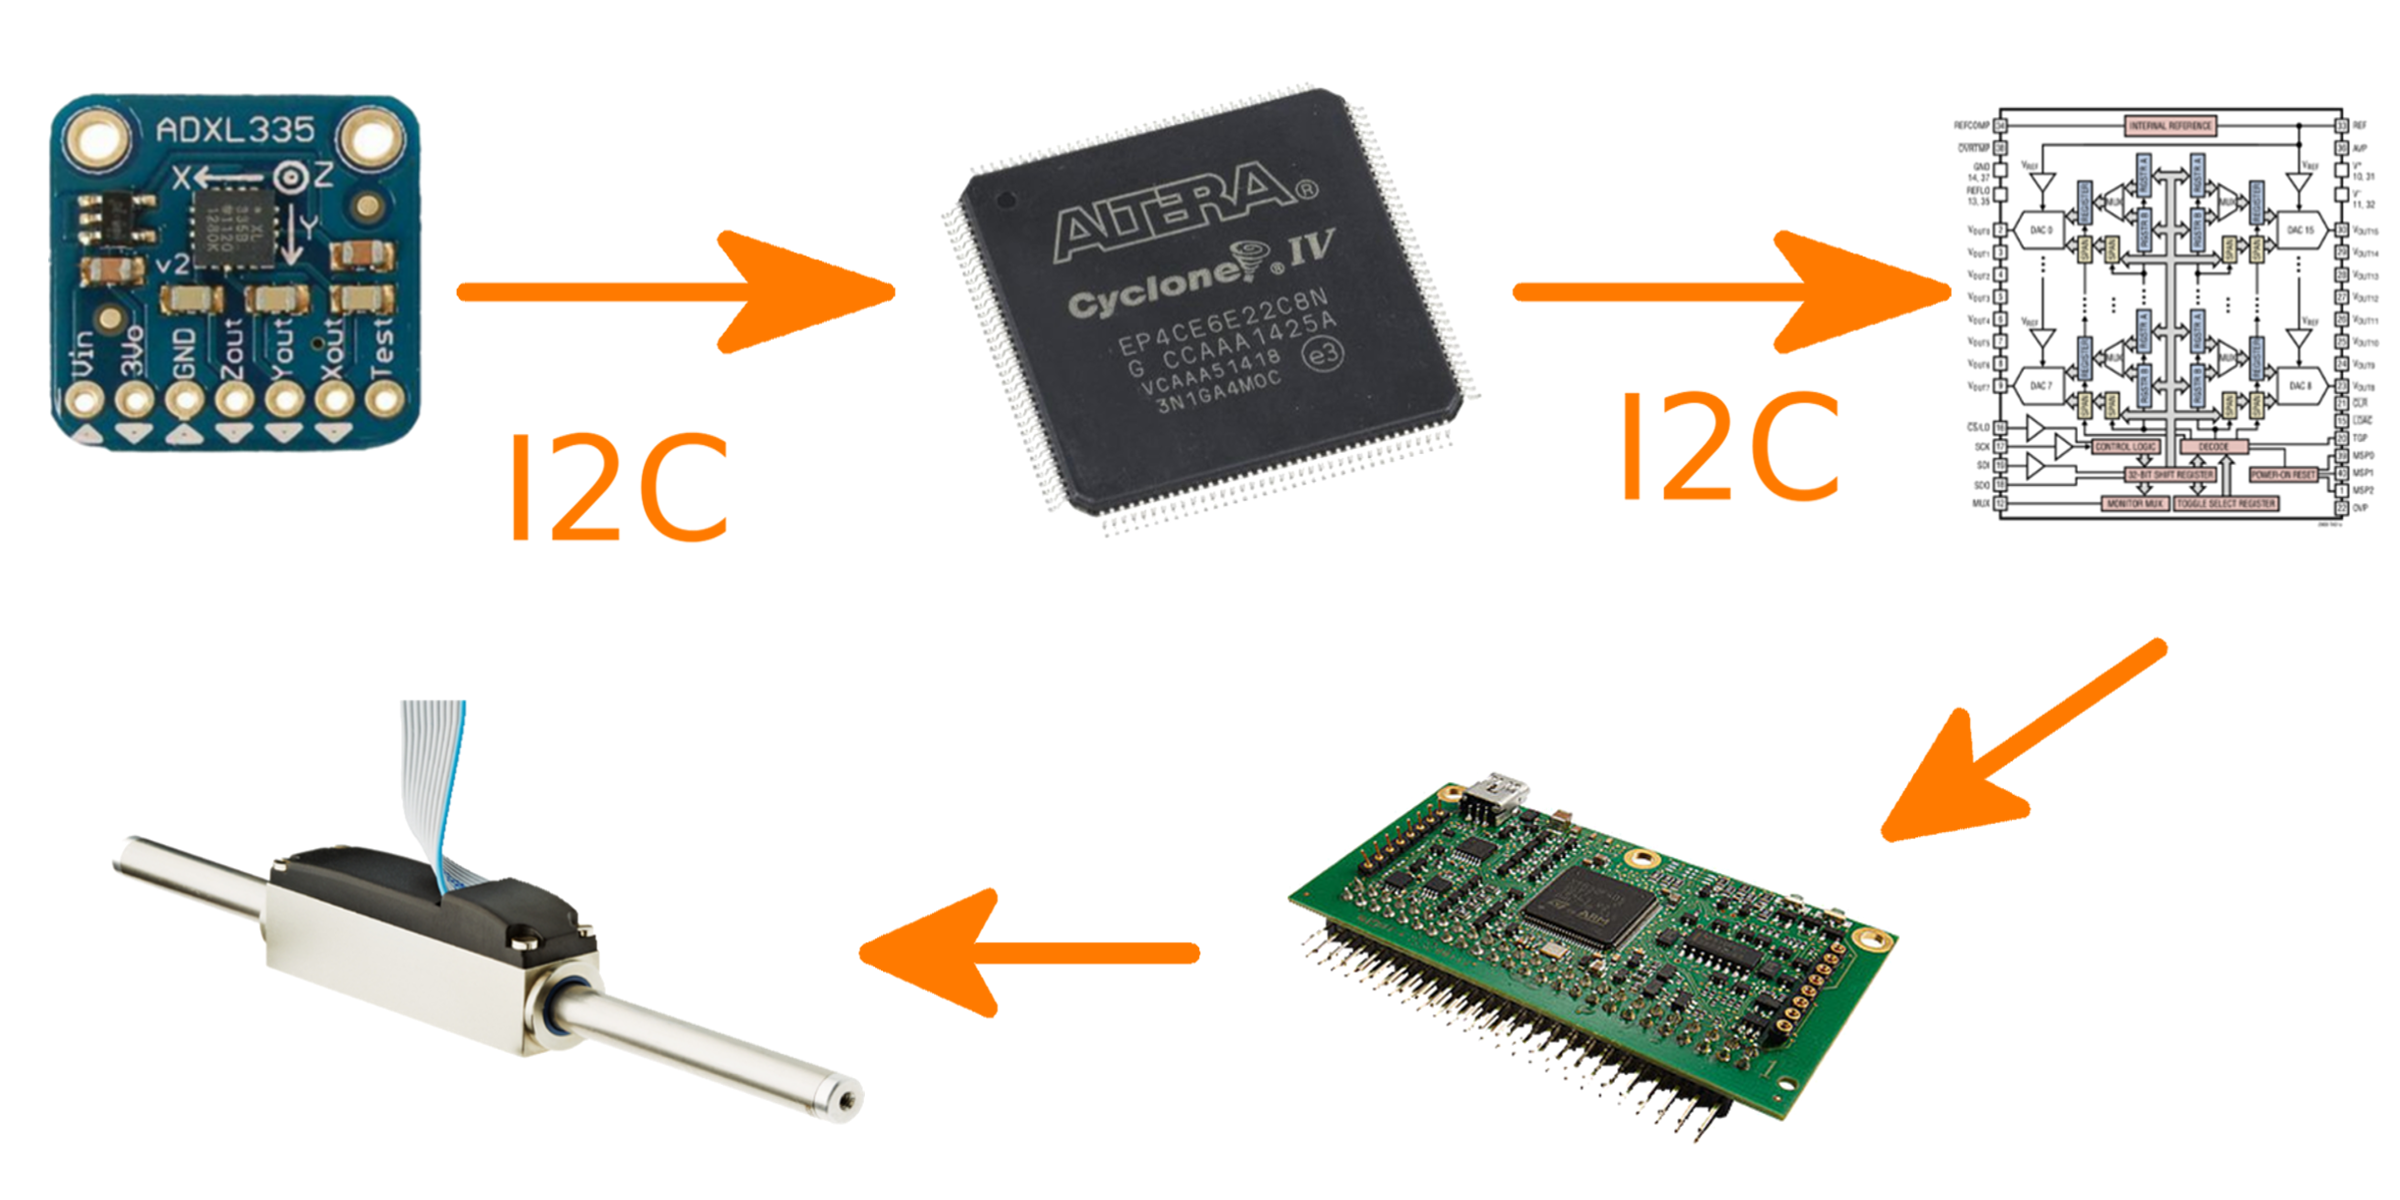
\includegraphics[width=15cm]{CH.png}\hss}\hfill\null
  	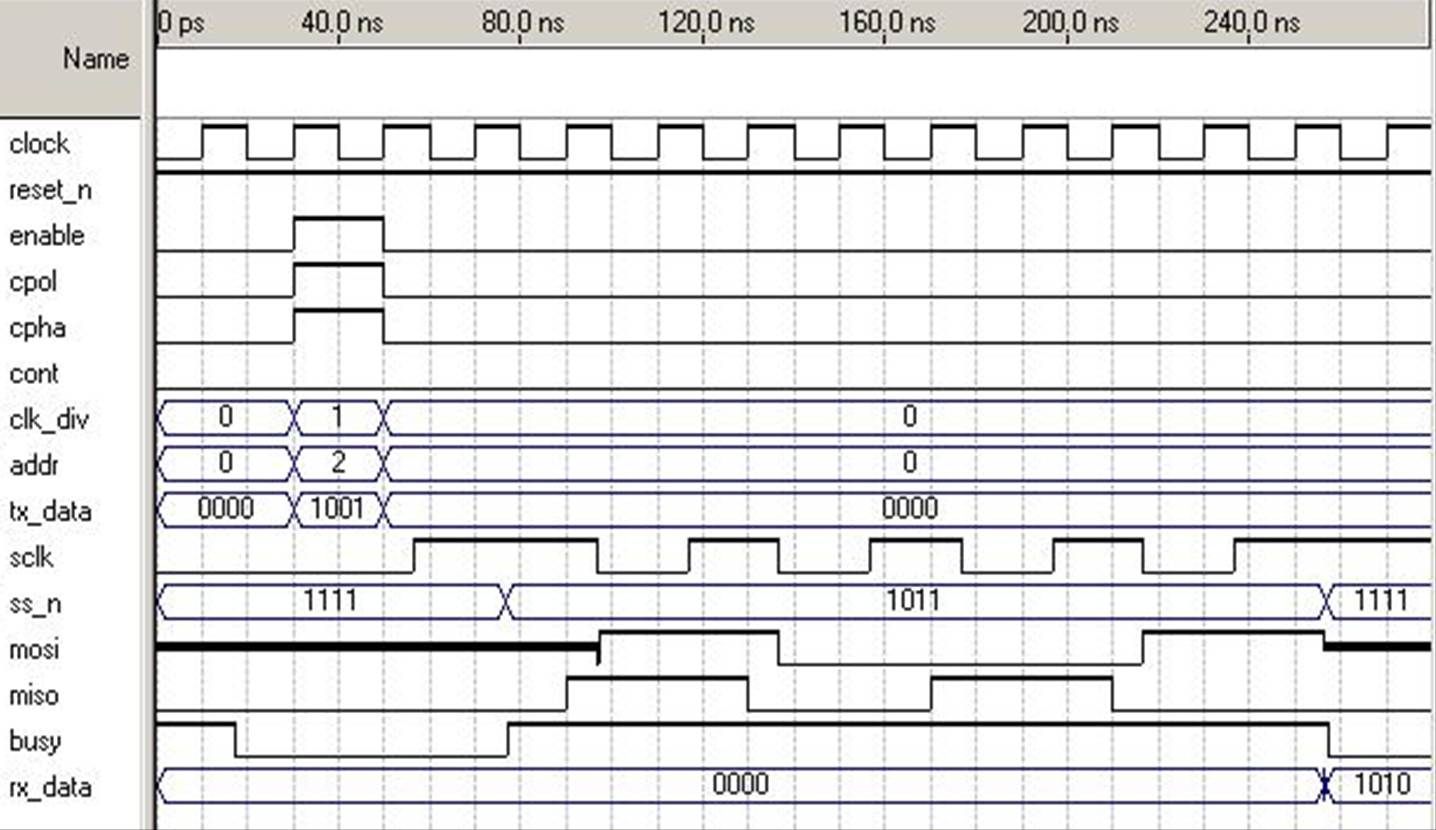
\includegraphics[width=12cm]{transaction_timing_diagram_web.JPG}
    \caption{diagramme d'état d'une transaction}
	\end{figure}
	
	\section{Modification}
		Une fois notre module pris en main, il nous a fallu le modifier afin de l'instancier avec l'utilisation des lignes miso et mosi mutualisées, mettant en oeuvre trois fils au lieux de quatre. Pour cela nous avons utilisé le mode haute impédance nécessaire à l'utilisation des ports en entrée sortie sur notre FPGA. Après avoir modifié le code afin de mutualiser les lignes miso et mosi, nous avons également dû adapter l'algorithme précédemment établi afin de mettre en haute impédance la ligne en fonction des besoins, afin que cette dernière ne soit pas bloquée lors d'une écriture ou d'une lecture de données. 
		
		Ainsi, lors d'une transaction, lorsque le nombre de bit total sera atteint, la ligne sera mise en haute impédance afin de libérer cette dernière pour une possible lecture.
		
	\begin{lstlisting}
 		void SensorInit()
		{
			--transmit spi clock toggle
					IF(assert_data = '1' AND clk_toggles < last_bit_rx) THEN
					  if (BITCOUNTER = 7 ) then
					  	tmp := tx_buffer(d_width-1);
					  end if;				
  	          if (BITCOUNTER >= 8 and tmp = '1') then
					  	MISOMOSI <= 'Z';				  
					  else 
					  	MISOMOSI <= tx_buffer(d_width-1);          --clock out data bit
					  	tx_buffer <= tx_buffer(d_width-2 DOWNTO 0) & '0'; --shift data transmit buffer				  
					  end if;				  
					  BITCOUNTER := BITCOUNTER +1;
					END IF;
		}
	\end{lstlisting}
	
	\section{Spi - application de plus "haut niveau"}
		Par la suite, nous avons instancié une application de plus haut niveau ayant comme rôle d'encapsuler notre module SPI ainsi que de nous permettre de configurer et d'adresser les registres souhaités de notre accéléromètre.
		
		\subsection{Encapsulation du module SPI MASTER}
			L'instantiation de notre module SPI MASTER reste trivial dans cette api, étant donné que nous avons simplement à configurer les différents ports et paramètre précédemment cité. Ainsi, le paramétrage s'effectue comme suivant:

	\begin{lstlisting}
 		sm_accel: entity work.spi_master(SPI_ACCEL)
  	GENERIC MAP(
   	 		slaves  => 1,
   	 		d_width => 16
	 		)
  	PORT MAP(
    	clock    => CLOCK_50,				-- clock system
    	reset_n  => reset_n,				-- signal de reset
    	enable   => spi_enable,			-- signal enable
    	cpol     => '1',						-- spi clock polarity
    	cpha     => '1',           	--spi clock phase
    	cont     => '0',         		--continuous mode command
    	clk_div  => 5,							--system clock cycles, based on 1/2 period of clock (~10MHz -> 3 ; 100K -> 250)
    	addr     => 0,             --address of slave
    	tx_data  => spi_txdata,    --data to transmit
    	sclk     => spi_sclk,      --spi clock
    	ss_n     => spi_ss_n,      --slave select
    	busy     => spi_busy,      --busy / data ready signal
    	rx_data  => spi_rxdata,			--data received
	 		MISOMOSI => GPIO_SPI_SDIO		--GPIO(2)
		);
		\end{lstlisting}
		
		\subsection{Accès aux registres de l'accéléromètre}
			Afin d'utiliser notre accéléromètre, nous avons à configurer divers registres pour que les données reçues soient conformes à l'utilisation que nous souhaitons faire de notre accéléromètre. C'est pourquoi, nous avons besoin d'effectuer les configurations suivantes:
			
			\begin{itemize}
				\item Avoir un intervalle de valeur évoluant de 0 à 8 g.
				\item Accéder aux registres contenant les valeurs échantillonnées par notre matériel sur l'axe des "Z"
				\item Configurer un bit d'état, permettant de savoir si la mémoire interne peut être accédée en lecture ou non.				
			\end{itemize}
			
			Pour cela, nous avons implémenté deux tableaux de registres, le premier contenant la configuration de l'accéléromètre et le deuxième contenant les registres à accéder en lecture.
		\begin{lstlisting}
 		constant ACCEL_CONFIG : T_WORD_ARR:= (
			7x"2D" & ADXL_WRITE_REG & 8x"01",		--initiate protocol configure registers (standby <- 1 : standby mode)
			7x"2F" & ADXL_WRITE_REG & 8x"52",		--Power-on reset, code 0x52		
			7x"2C" & ADXL_WRITE_REG & 8x"03",		--G range [+-8g : 3] ; [+- 4g : 2] ; [+-2g : 1] ; [disable : 0]
			7x"28" & ADXL_WRITE_REG & 8x"00",		--HPF [0.238 : 6] ; [0.954 : 5] ; [3.862 : 4]
			7x"2D" & ADXL_WRITE_REG & 8x"00"			--End protocol configure registers (standby mode <- 0 : mesurement mode)
			);
			
		constant ACCEL_READ : T_WORD_ARR:= (
			ADXL_DATAZ1_ADD & ADXL_READ_REG & 8x"00", 	-- DATAZ1 (MSB) - 2100
			ADXL_DATAZ2_ADD & ADXL_READ_REG & 8x"00", 	-- DATAZ2		 		- 1F00
			ADXL_DATAZ3_ADD & ADXL_READ_REG & 8x"00", 	-- DATAZ3 (LSB)	- 1D00
			ADXL_STATUS_ADD & ADXL_READ_REG & 8x"04"		-- NVM_BUSY to check if memory can be access
			);
		\end{lstlisting}
		
		Ces deux tableaux ainsi que le module SPI MASTER sont mis en application au travers de la machine d'état que nous allons maintenant décrire. Machine d'état pouvant être interprétée comme l'algorithme de ce module de plus haut niveau.			
		
		\subsection{Intégration globale - Machine d'état}
				Au travers de la machine d'état ci-dessous, nous pouvons observer le comportement de notre module, pour que ce dernier puisse interagir avec notre accéléromètre au travers de l'envoi et de la réception de données.
		
			\begin{figure}[!ht]
    		\center
   		 	%\hfill\hbox to 0pt{\hss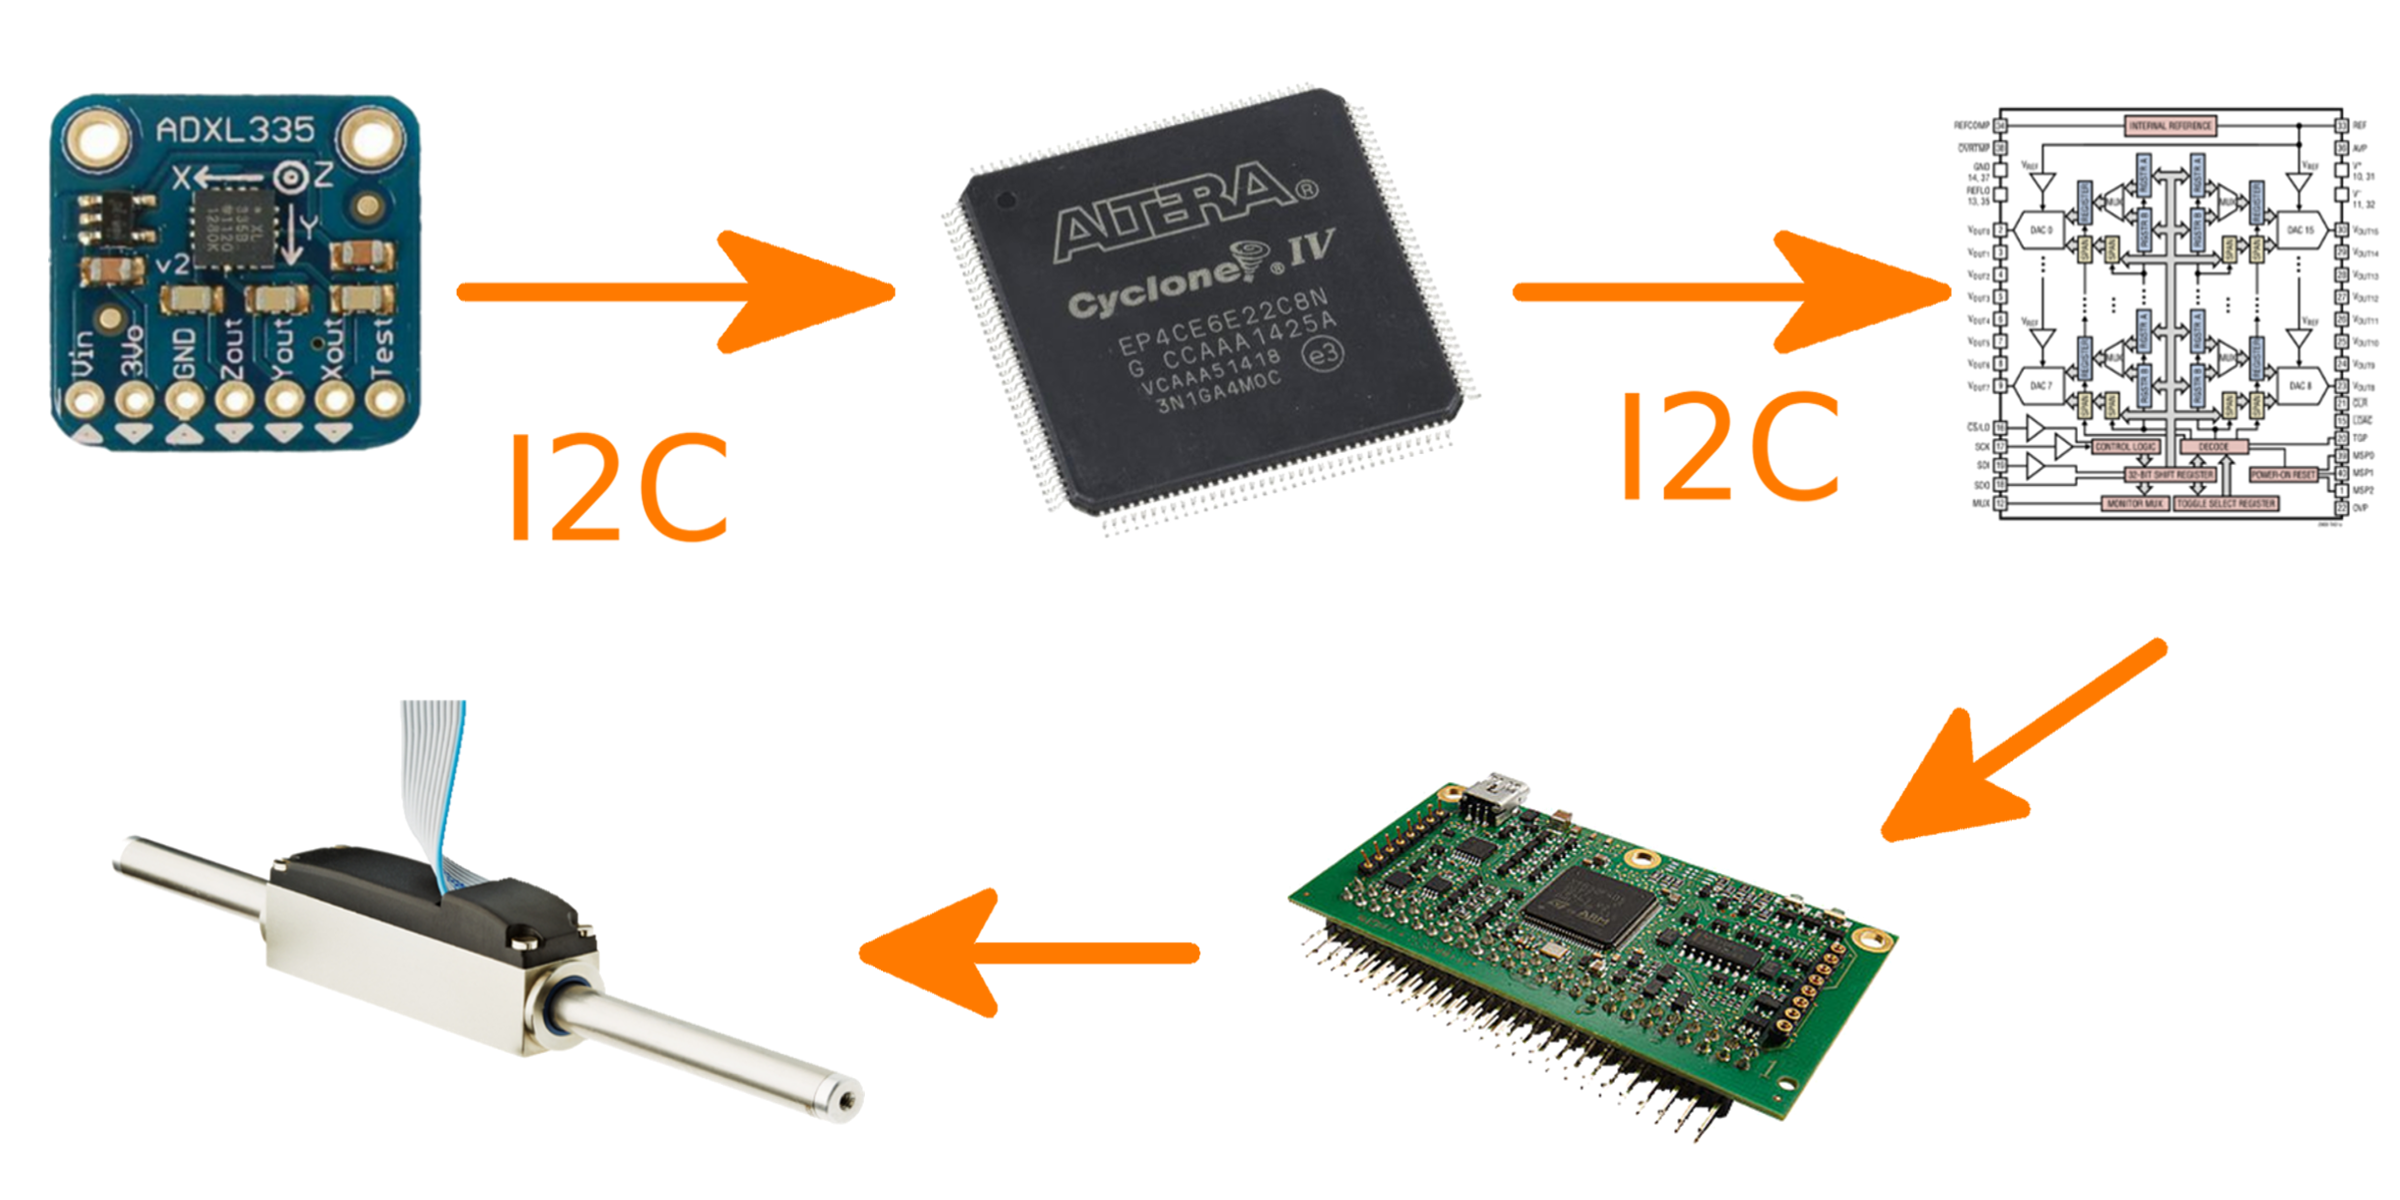
\includegraphics[width=17cm]{CH.png}\hss}\hfill\null
  			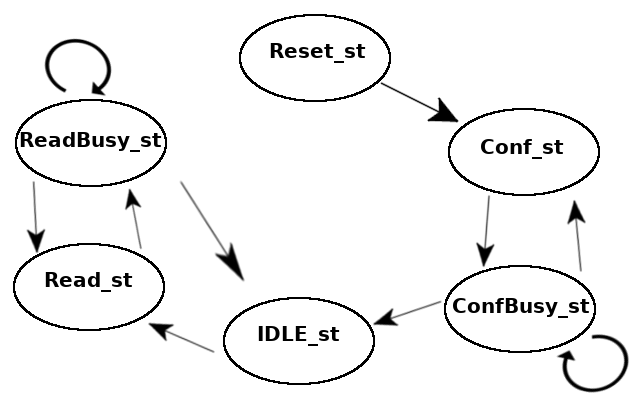
\includegraphics[width=10cm]{acc_StateMach.png}
    		\caption{Machine d'état - module accéléromètre}
			\end{figure}
			
			On retrouve ainsi un premier état, "Reset\_st", qui nous permet de réinitialiser notre module et ainsi notre communication. Ensuite, viennent les états de configuration "Conf\_st" et "ConfBusy\_st" au travers desquels nous configurons les registres de l'accéléromètre que nous avons décrits plus tôt. Puis vient un état d'attente "Idle\_st", état dans lequel l'accéléromètre se met en attente d'un évènement, qui dans notre cas va être le déclenchement d'une demande de lecture des données échantillonnées par l'accéléromètre. Enfin, nous retrouvons les états de lecture "Read\_st" et "ReadBusy\_st"; "Read\_st" permettant l'accès à un registre de valeur, puis basculant en "ReadBusy\_st" afin de déterminer s'il reste ou non un registre à lire. Pour finalement retourner en état d'attente lorsque les trois registres, de 20 bits en tout formant la valeur échantillonnée, auront été lus.		
	
	\chapter{Le filtrage}
	
	\section{Etat de l'art}
	Au sein de la chaîne, le module de filtrage est la clef de voute de cette dernière. C'est au sein de ce module que va être intégrée la partie de traitement du signal, que nous aborderons par la suite. Le traitement du signal prend place au travers d'une fonction de transfert, devant nous permettre de moduler notre signal en fonction de la courbe de réponse souhaitée pour notre chaîne.
	
	En attendant que cette fonction de transfert soit déterminée grâce à la manipulation sur le banc de test (que nous décrirons également plus tard), nous avons un module ayant un rôle simple et précis, copier les données qu'il reçoit en entrée, traiter ces dernières codées en complément à deux afin qu'elles puissent être interprétées par notre DAC n'acceptant que des données non signées sur 16 bits. Notre module se base donc sur une machine d'état relativement simple.
	
	Lors du premier état "IDLE\_st", nous attendons qu'une donnée soit adressée au module et lorsque c'est le cas, nous effectuons un cast sur notre donnée codée sur 20 bits, afin de travailler sur un mot de 16 bits, composé des 16 MSB du mot précédent, à destination du DAC. Ensuite, nous appliquons un offset afin de décaler notre mot complémenté à deux (évoluant de -32768 à +32767) afin que ce dernier devienne un mot non signé, codé de 0 à 65535.
	
	\chapter{Du FPGA au CNA}
	
	\section{Mise au point}
	
	Pour ce dernier module de la chaîne de contrôle, nous avons à mettre en place la communication entre le FPGA et notre DAC via une liaison SPI. Etant donné la nature de la transmission, nous n'avons pas besoin de mettre au point une nouvelle machine d'état. Assurant une liaison SPI, nous pouvons réutiliser notre code, développé pour la transmission entre l'accéléromètre et le FPGA. La seule modification à apporter est l'ajout d'un état nous permettant d'adresser un registre particulier sur le DAC, correspondant à l'une des lignes de sortie en tension du DAC. Cet état se comporte donc comme suivant.
	
	Lorsque nous arrivons en transmission, nous concaténons quatre bits de poids fort correspondant à une configuration de registre permettant un swap instantané entre l'entrée et le registre de contrôle, à la suite desquels nous ajoutons encore quatre bits correspondant à l'adresse de la ligne de sortie en tension. Enfin, sont ajoutés à la suite les 16 bits de données à transmettre.
	
		\begin{lstlisting}
 			when TRANSMITst =>
					fifo_oe_w <= '0';
					spi_txdata(15 downto 0)	 <= fifo_read;
					spi_txdata(19 downto 16) <= SPI_CONFIG(1);
					spi_txdata(23 downto 20) <= SPI_CONFIG(0);
					
					cState <= TRANSMITCONFst;
		\end{lstlisting}
		
		Ainsi, en réadaptant notre api encapsulant le module "SPI MASTER", nous avons pu aisément remettre en place une liaison SPI vers un nouveau device.
		
		\section{Difficulté rencontrée}
		
		Par la suite, alors que nous souhaitions mettre en place notre chaîne de contrôle, afin de réaliser des tests sur notre maquette de piano, nous nous sommes aperçus d'un problème non pas sur la propagation des données, mais sur la stabilité du signal électrique de ces dernières. En effet, notre moteur réagissait aux impulsions mesurées par notre accéléromètre, mais ce dernier restait très peu stable et oscillait de manière aléatoire.
		
		Ainsi, afin de déterminer la cause du problème, nous avons cherché à visualiser nos signaux à l'aide d'un oscilloscope et nous avons obtenu les graphiques ci-dessous. Pouvant observer notre signal "bruité", nous avons cherché à déterminer la cause de ce problème.
		
		\begin{figure}[!ht]
    \center
   	%\hfill\hbox to 0pt{\hss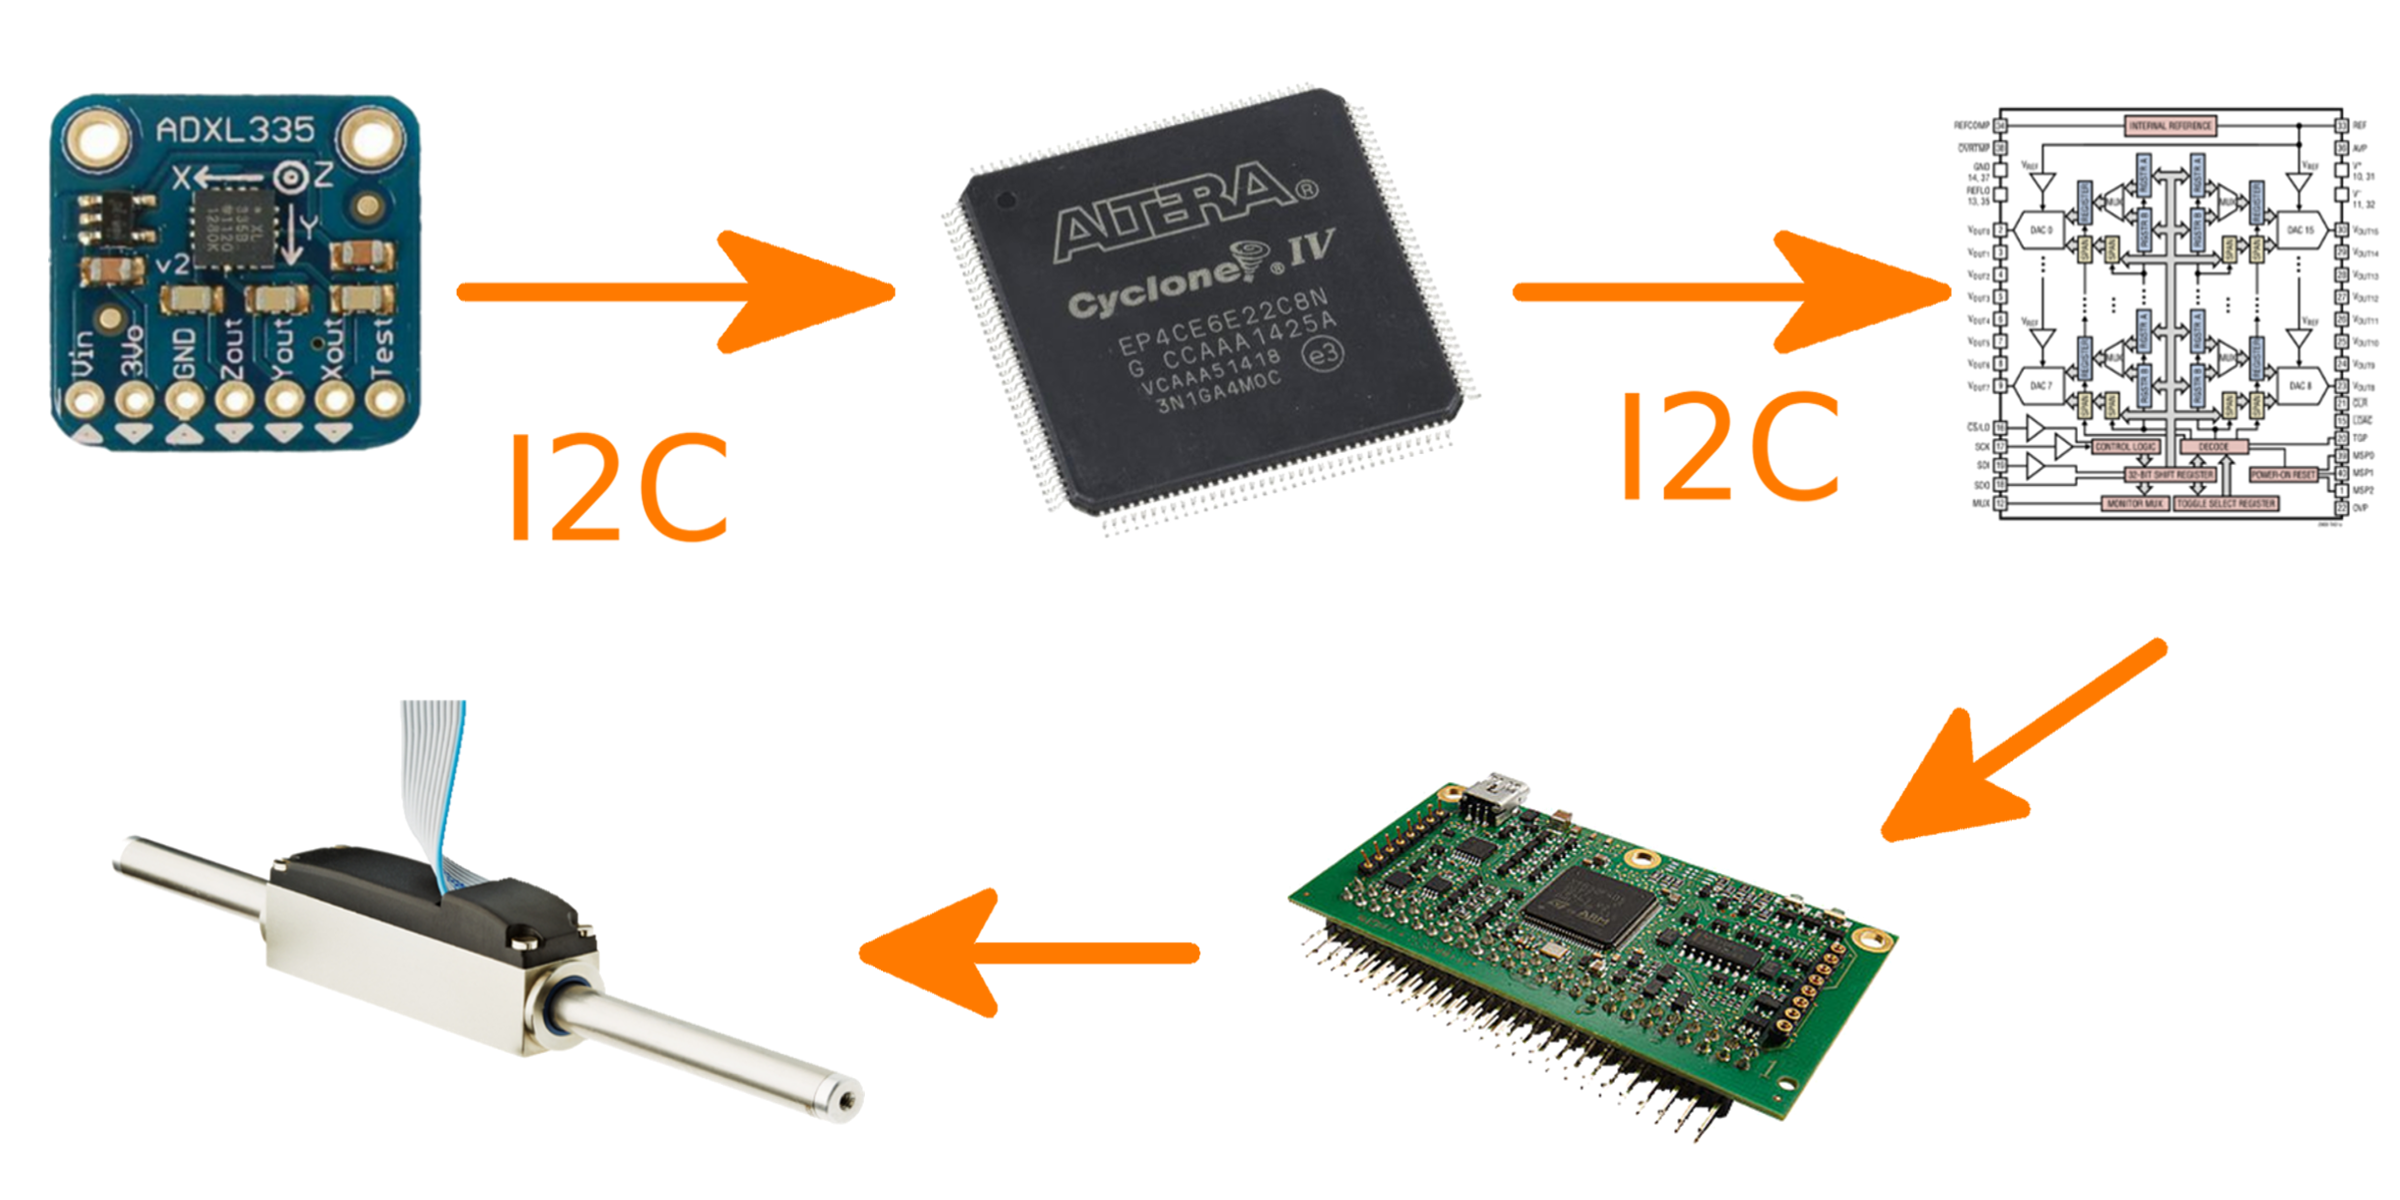
\includegraphics[width=17cm]{CH.png}\hss}\hfill\null
  	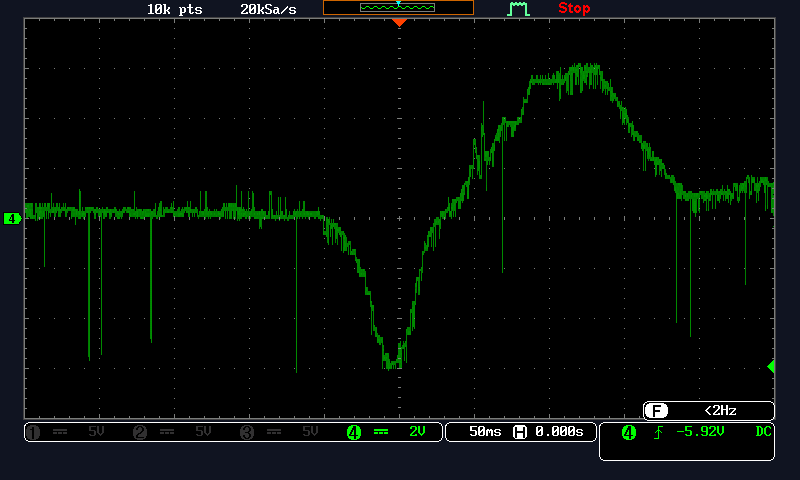
\includegraphics[width=10cm]{bruit1.PNG}
		\caption{Stabilité - graphique 1}
	\end{figure}
	
	Dans un premier temps, étant donné que nous travaillions sur un prototypage rapide, nous avions beaucoup de câbles connectés à l'aide de connecteurs rapides, ce qui pouvait être source de problème. Nous avons donc éliminé cette possibilité en concevant une carte "mezzanine" (carte que nous détaillerons lors d'un prochain chapitre) afin de disposer de branchements toujours amovibles, mais d'une plus grande qualité.
	
	N'ayant toujours pas résolu notre problème, nous nous sommes tournés, cette fois, du côté de la propagation du signal électrique au sein du FPGA, à l'aide d'un outil de diagnostique interne "signal tap". À l'aide de cette oscilloscope numérique, nous avons pu remonter notre signal jusqu'à l'apparition du bruit, nous conduisant à une FIFO au sein du module DAC.
	
	Cette FIFO fut développée alors que j'avais peu de connaissance vis-à-vis du langage VHDL et de ces spécificités, afin de m'exercer. Ce qui me conduisit dans un "piège" de débutant, non visible lors de la phase de débug sous ModelSim. En effet, l'outil de débug nous permet de simuler nos scripts, mais il reste une simulation, si bien qu'une recopie déclenchée par un front montant d'une horloge système apparait comme fonctionnelle, alors qu'en application, il nous faudrait attendre que le front d'horloge soit passé, puis teste l'état de cet "oenable" pour ensuite effectuer notre copie.
	
	Ce mécanisme de conception se nomme la métastabilité.
	
	Afin de remédier rapidement à ce problème, nous avons choisi d'implémenter une FIFO, mise à disposition par le framework du constructeur de la carte, éliminant ainsi tout problème de métastabilité.		
		
	\chapter{Une octave "augmentée"}
		Après avoir mis au point cette première manipulation, devant mettre en oeuvre l'action d'une touche de piano, entrainant la frappe d'une corde; l'ensemble étant fonctionnel et ayant démontré la preuve de concept, nous allons maintenant chercher à généraliser cette chaîne sur un mécanisme composé de douze touches.
		
		Cette généralisation ayant été prévue dès le début du projet, le découpage de ce dernier en module, reste très avantageux. En effet, utilisant maintenant douze touches, il nous faut récupérer les données provenant de douze accéléromètres et donc appliquer douze filtrages numériques indépendants. Pour cela, nous pouvons donc réutiliser nos deux premiers modules (accéléromètre et Filtre) que nous allons dupliquer à l'aide d'une fonctionnalité fournie par le langage VHDL, les "GENERATE".
		
		Cette fonction, nous permet de pouvoir dupliquer un élément de code, dans notre cas, douze fois; et c'est là que tout l'intérêt du VHDL apparait. Si nous avions implanté notre projet sur un micro-processeur, ces douze modules auraient fonctionné de manière sérialisée. Ici, grâce au VHDL, ces douze modules vont fonctionner de manière parfaitement parallèle, ainsi, si deux touches sont jouées en même temps, les informations relatives à celles-ci se propageront simultanément.
		
		La seule modification majeure qui va devoir être apportée, va être sur le dernier module, devant pouvoir stocker simultanément les informations de douze modules, pour ensuite sérialiser ces dernières, une par une, sur la ligne à destination de la communication SPI.
		
		\newpage
		
	\section{Modification du module DAC}
		Devant maintenant récupérer les informations en provenance de douze accéléromètres et possiblement de manière simultanée, il nous faut adapter notre dernier module. Là où notre première implémentation se reposait sur la recopie d'une entrée sur une sortie lors d'un acquittement signifiant qu'une donnée était disponible, il nous faut maintenant travailler avec notre douzaine de modules ainsi que les acquittements certifiant la disponibilité de nouvelles données.
		
		Afin de nous contraindre à nos nouvelles contraintes, nous avons mis en place une architecture basée sur un empilement de FIFO à horloge mixte. La logique de notre nouvelle architecture est illustrée sur la figure suivante.
		
	\begin{figure}[!ht]
    \center
   	%\hfill\hbox to 0pt{\hss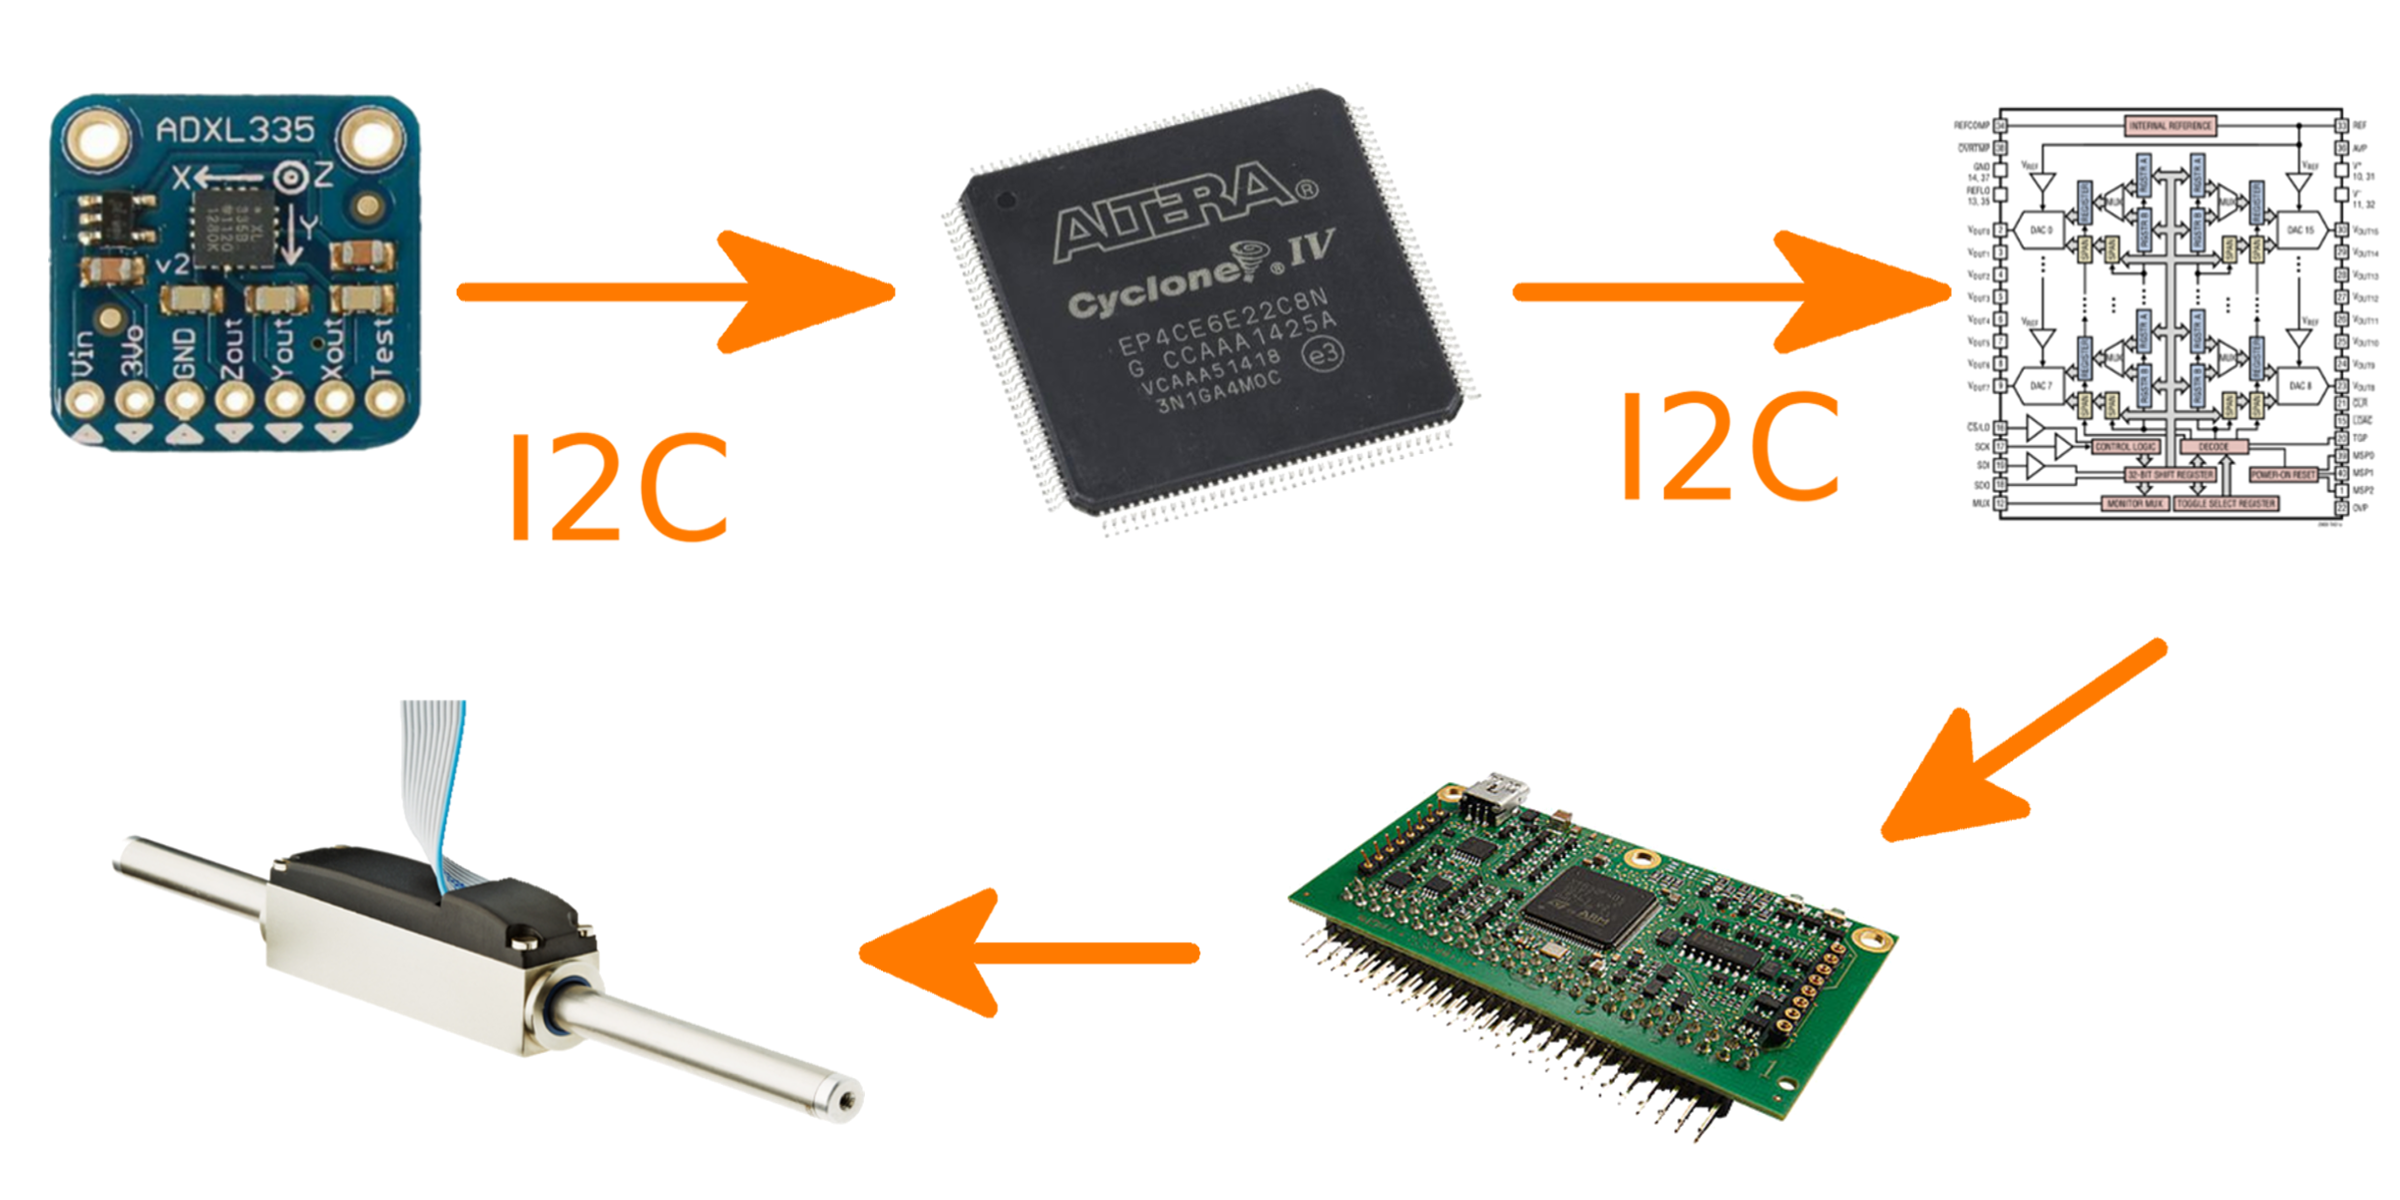
\includegraphics[width=17cm]{CH.png}\hss}\hfill\null
  	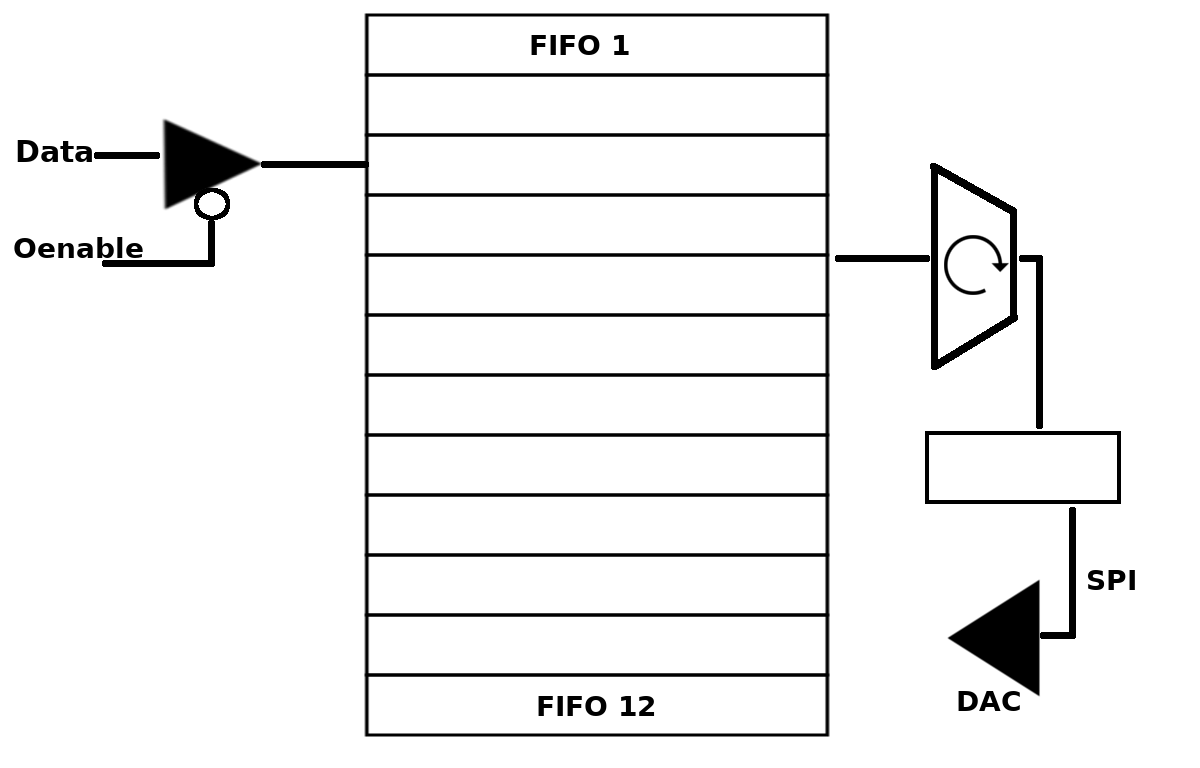
\includegraphics[width=12cm]{octave.png}
		\caption{Une octave "augmentée" - Architecture}
	\end{figure}
		
		Comme nous pouvons le voir sur la figure ci-dessus, cette nouvelle architecture se base sur un ensemble de douze FIFO pouvant être accédé de manière indépendante par chacun des modules auxquel cette dernière est rattachée. Ensuite, nous exploitons encore une fois la spécificité du langage VHDL au travers d'une boucle "for" qui nous permet de pouvoir parser l'ensemble des FIFO sur un seul coup d'horloge du système (horloge ayant une fréquence différente de celle permettant le stockage des données dans les FIFO.
		Grâce à ce mécanisme, nous pouvons, pour chaque coup d'horloge, parser l'ensemble de nos FIFO, afin de déterminer si de nouvelles données sont disponibles, pour ensuite les sérialiser sur une dernière FIFO reliéee à une api encapsulant le bus SPI qui va permettre l'envoi des données au DAC.
		
		Cette architecture n'a pas pu être testée en condition, sur la maquette, elle n'a pour l'instant été testée qu'en simulation sous l'outil de modélisation "ModelSim". Bien que permettant une simulation au plus proche des conditions réelles, il nous faudra valider ce modèle en phase de test, pour ainsi déterminer si les contraintes de temps et de propagation des données sont respectées; le cas échéant, il nous faudra mettre au point une architecture plus subtile.
		
		\section{Ouverture}
		
		Maintenant que notre chaîne de contrôle est fonctionnelle et que nous avons vu comment adapter son architecture afin d'évoluer vers un banc de test plus complet comprenant une douzaine de touches, il nous faut à présent penser aux améliorations futures qui, sans "dénaturer" le modèle existant, nous permettrait d'apporter une valeur ajoutée au projet.
		
		C'est dans cet esprit que nous pourrions mettre en place une solution de monitoring, afin de pouvoir suivre en temps réel, l'évolution du signal au fur et à mesure de la chaîne, afin de valider son traitement ainsi que son bon "comportement", sans avoir à passer par des outils de mesure difficilement transportables et encombrants.
		
	\begin{figure}[!ht]
    \center
   	%\hfill\hbox to 0pt{\hss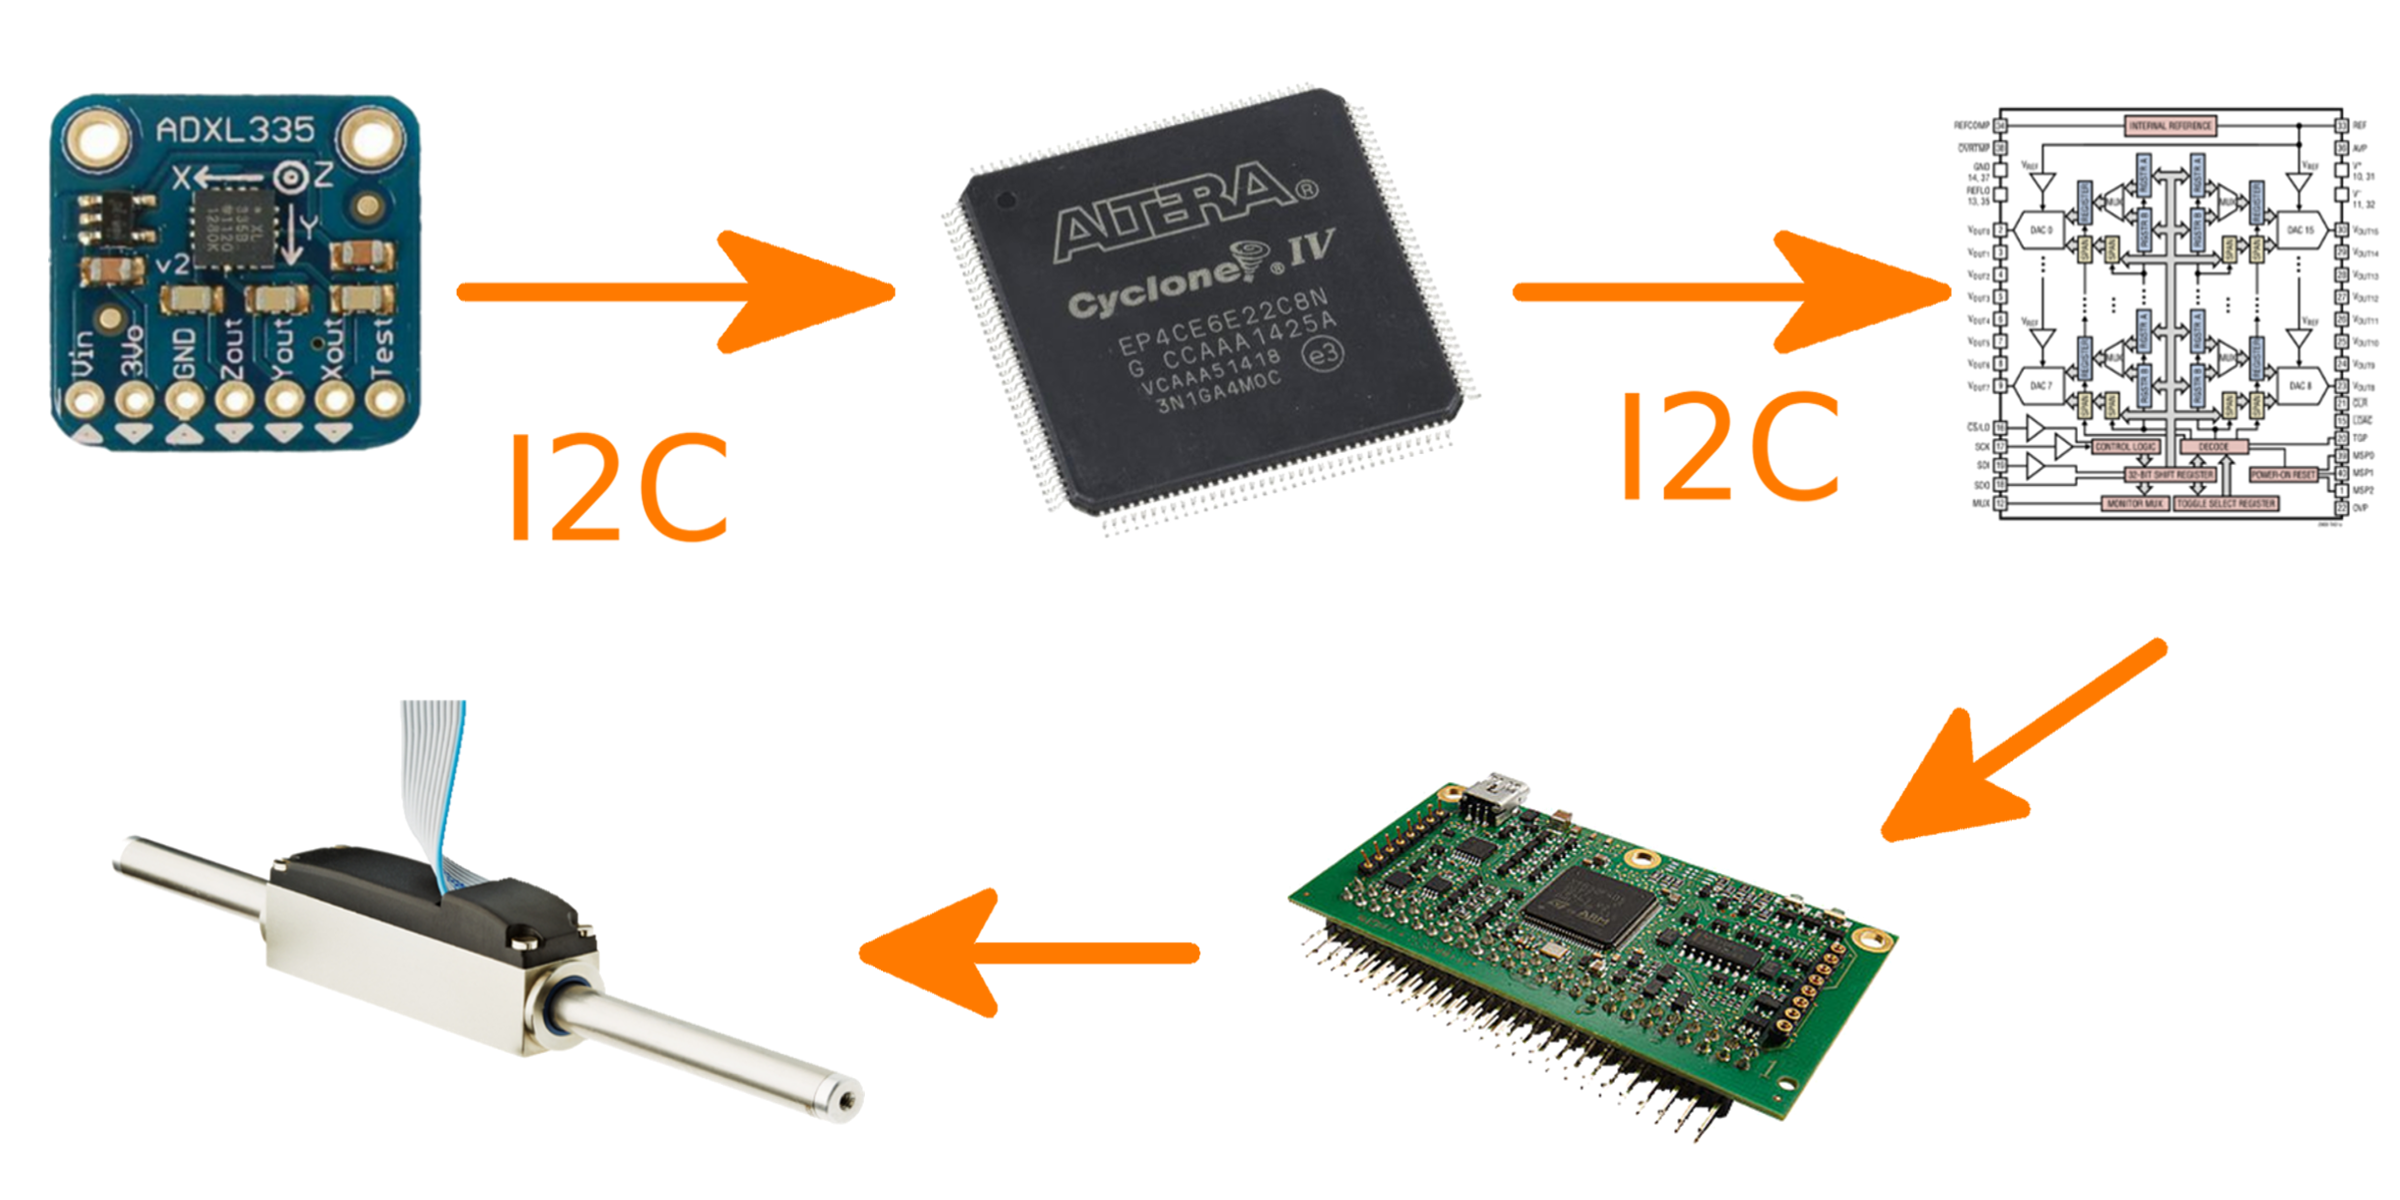
\includegraphics[width=17cm]{CH.png}\hss}\hfill\null
  	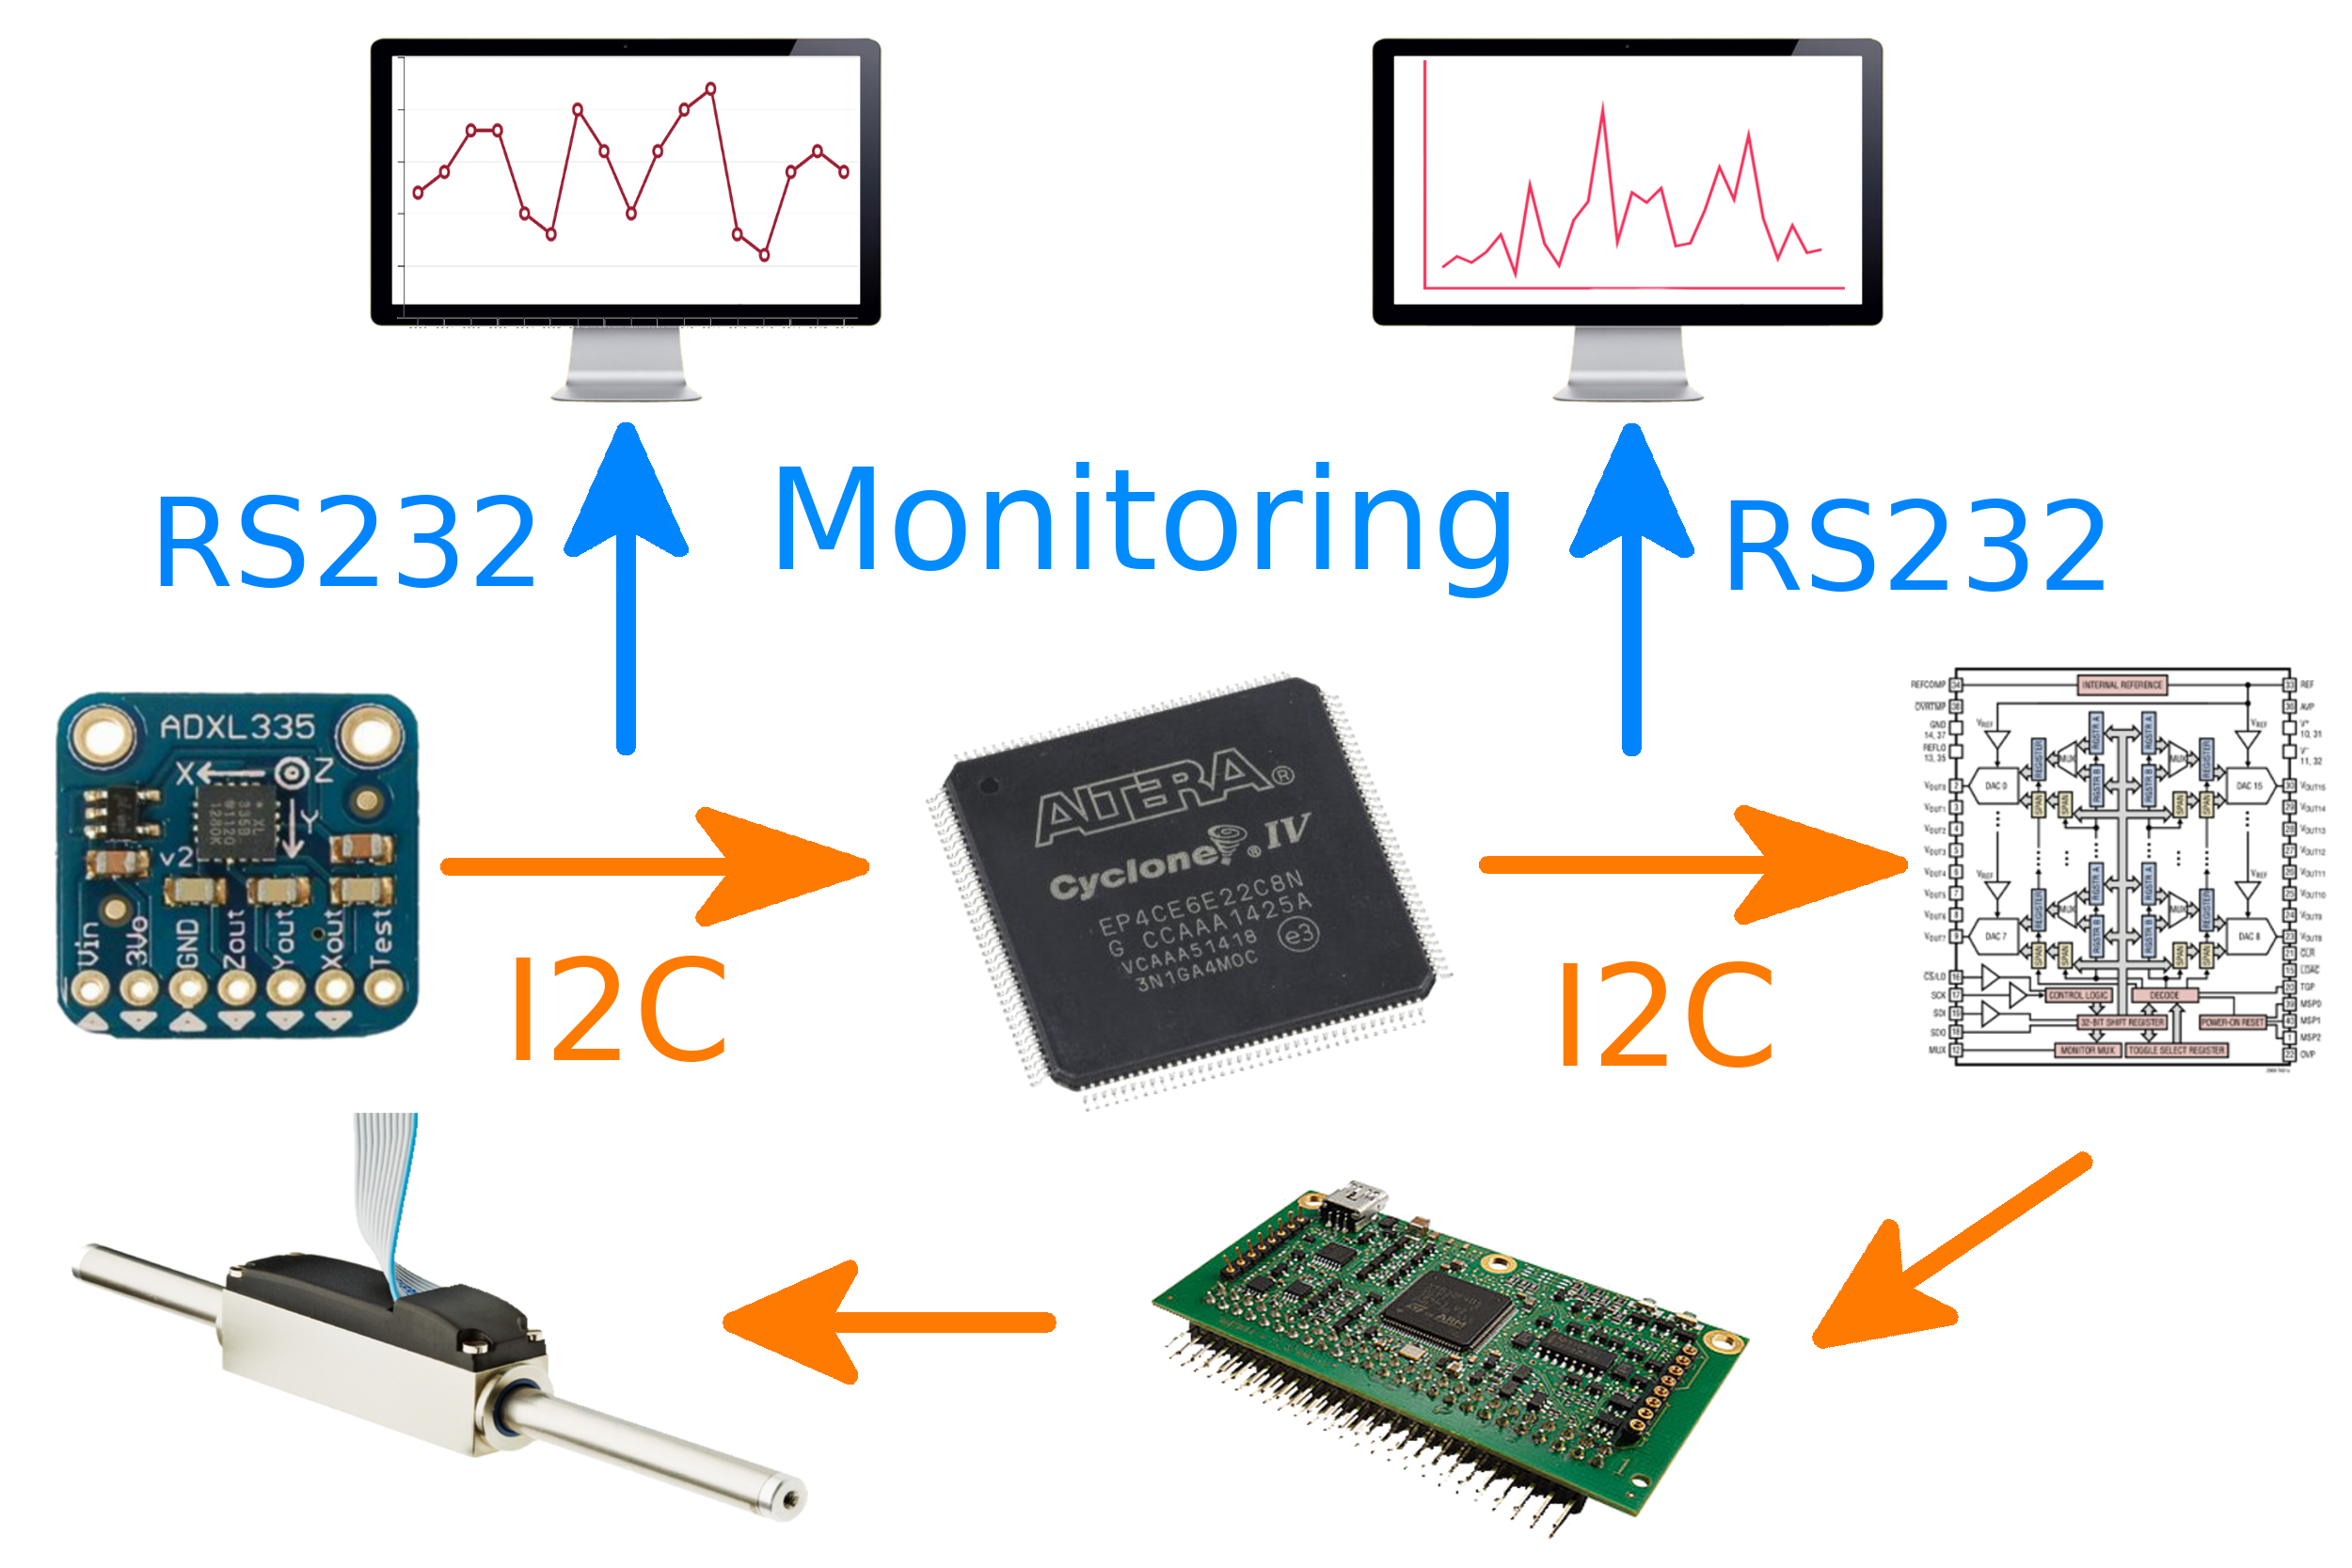
\includegraphics[width=12cm]{CH&MO.png}
		\caption{Chaîne de contrôle - Monitoring des informations}
	\end{figure}
		
	Ci-dessus se trouve la maquette imaginée afin de monitorer le signal en provenance des accéléromètres avant et après l'étape de filtrage numérique, nous permettant ainsi, comme dit plus haut, de caractériser et valider notre modèle.



%--------------------------------------------------------------------------------------
%
%	Asservissement et caractérisation
%		Fonction de transfert

%		Manipulation en laboratoire
%
%--------------------------------------------------------------------------------------
	\part{Asservissement et caractérisation}
	
	Lors de la précédente partie, nous avons abordé l'ensemble des aspects qui nous ont permis de mettre au point notre chaîne de contrôle; en partant des données fournies par notre accéléromètre, leurs réceptions et leurs traitements au sein de notre carte programmable (FPGA), jusqu'à leur envoi et leur réception par le Convertisseur Numérique Analogique, permettant le contrôle du contrôleur moteur, en lui transmettant des consignes de fonctionnement.
	
	Lors de cette partie, nous allons nous concentrer sur la mise au point de l'asservissement numérique, élément indispensable, devant prendre place au sein du filtre numérique de notre carte programmable FPGA.
	
	L'asservissement numérique est un processus en plusieurs étapes, consistant à piloter un système tiers, en mesurant périodiquement des valeurs de consigne, fournies par un système de capteurs, dans notre cas, un accéléromètre. 
	Par la suite, ces données sont traitées par notre calculateur, mais étant donné le mode de traitement des informations imposées par notre calculateur qui est de nature numérique et cadencé dans le temps de façon périodique grâce à une horloge; les informations en entrée, provenant de nos capteurs, sont donc des grandeurs discrètes.
	
	Les différentes étapes que l'on retrouve, générique à tout système asservi sont les suivantes:
	
	\begin{itemize}
		\item l'échantillonnage d'un signal continu
			Cette opération consiste à relever les informations prises par un signal continu à intervalles de temps
			régulier, appelé période d'échantillonnage. On parle alors de signal échantillonné, signifiant que le
			calculateur ne tiendra compte que des valeurs prises par le calculateur aux instants d'échantillonnage.
			
		\item La conversion d'un signal analogique en un signal numérique
			Il s'agit de convertir la valeur prise par un signal analogique à l'instant d'échantillonnage en une
			valeur numérique, afin qu'elle puisse être traitée par le calculateur. Un tel signal peut, par exemple, 
			provenir d'un capteur. On parlera alors de signal de mesure.
			 
		\item La conversion d'un signal numérique en un signal analogique
			Cette opération consiste à transformer le signal numérique issu du calculateur à l'instant 
			d'échantillonnage (on parlera de signal numérique de commande), en signal analogique de commande 
			existant sur toute la période d'échantillonnage, l'objectif étant de commander le système physique.
			
		\item  La synthèse d'un algorithme de calcul
			Il s'agit d'établir une loi d'évolution du signal de commande numérique en fonction des signaux de mesure
			et de référence, également numériques, afin de permettre au système asservi de satisfaire un cahier des
			charges. Cette fonction est appelée correcteur numérique ou encore loi de commande numérique. Elle a pour
			objectif de déterminer la valeur du signal numérique de commande à un instant d'échantillonnage, à partir 
			d'un algorithme de commande, de mesure et de référence.
	\end{itemize}
	
	Ainsi, l'on peut résumer sous forme de schéma bloque une structure classique d'asservissement numérique comme suivant:
	
%	\begin{figure}[!ht]
%    \center
%    %\hfill\hbox to 0pt{\hss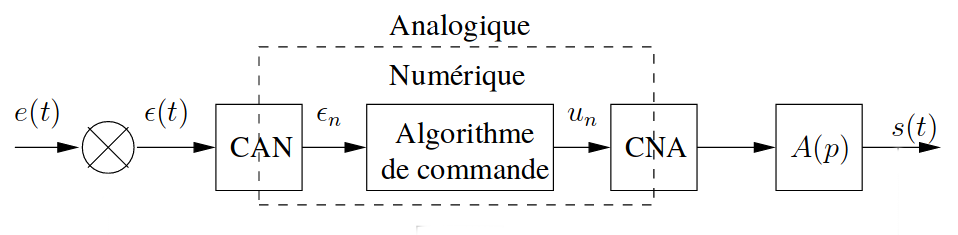
\includegraphics[width=17cm]{Assert_1.png}\hss}\hfill\null
%  	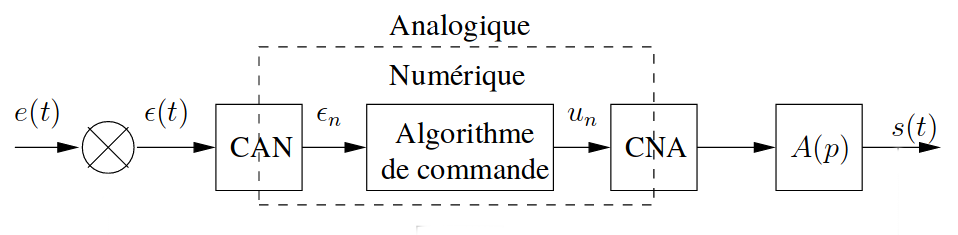
\includegraphics[width=17cm]{Assert_1.png}
%    \caption{Structure classique d'asservissement numérique}
%	\end{figure}	
	
	De plus, l'asservissement numérique de notre projet implique la caractérisation de la fonction de transfert de notre système dans son ensemble.
	Ainsi, afin de déterminer notre fonction de transfert, seront présentés les différents protocoles et les différentes manipulations effectuées sur notre banc de test.

	\chapter{Asservissement du projet Champ}
	
		Au sein de notre projet, notre asservissement va reprendre les différentes étapes présentées ci-dessus. Ainsi, concernant l'échantillonnage d'un signal continu, cette étape est réalisée au sein de notre accéléromètre étant donné que ce dernier nous fournit un signal échantillonné à une fréquence de 1 KHz (Période d'une milliseconde). Notre accéléromètre disposant d'un convertisseur analogique numérique intégré sur chaque axe, c'est au sein de ce dernier que s'effectue l'opération d'échantillonnage du signal continu.
		
		Par la suite, c'est au sein de notre carte programmable FPGA que s'effectue la phase de traitement sur notre signal discret. C'est au sein de notre filtre numérique que va être appliqué l'algorithme de synthèse sur les mesures en provenance de l'accéléromètre, afin d'asservir le système contrôlé, selon le cahier des charges.
				
		Enfin, la fonction de conversion de notre signal numérique en un signal analogique est assurée par le convertisseur numérique analogique (CNA) ayant pour rôle de fournir une commande au contrôleur moteur, existant sur toute la période d'échantillonnage, afin de commander notre système physique.
		
		Comme précédemment, on peut résumer l'asservissement mis en place pour le projet CHAMP, sous la forme d'un schéma bloc, comme suivant:
		
	\begin{figure}[!ht]
    \center
    %\hfill\hbox to 0pt{\hss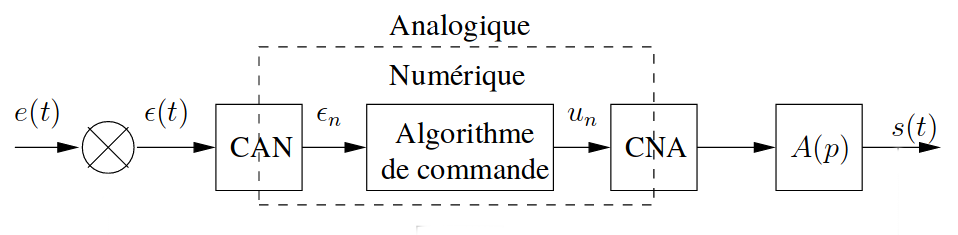
\includegraphics[width=17cm]{Assert_1.png}\hss}\hfill\null
  	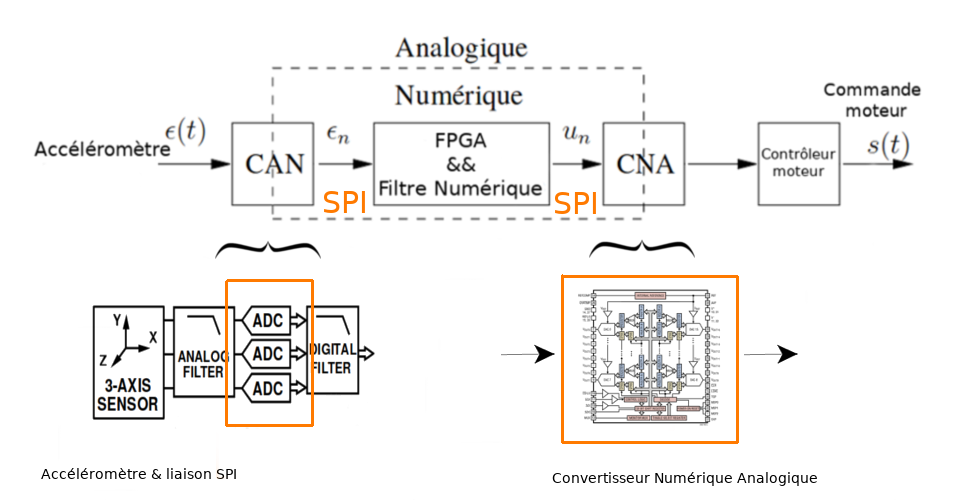
\includegraphics[width=12cm]{Assert_2.png}
    \caption{Asservissement numérique du projet CHAMP}
	\end{figure}	
		
		
	\chapter{Fonction de transfère}
	
		La fonction de transfert de notre système correspond à l'algorithme, appliqué sur nos données (discrètes) au sein du filtre. Une fois les données sorties de cet algorithme, les données sont aptes à piloter notre système tiers comme nous le souhaitons.
		
		Une fonction de transfert est le modèle mathématique de la relation entre la sortie et l'entrée de notre système ; le plus souvent cette fonction étant invariante en fonction des paramètres d'entrer.
		Du point de vue d'une approche physique, la fonction de transfert caractérise la dynamique du système; elle ne dépend que de ses caractéristiques physiques. 
		Ainsi, un système sera décrit par sa fonction de transfert et représenté comme suivant:

	\begin{figure}[!ht]
    \center
    %\hfill\hbox to 0pt{\hss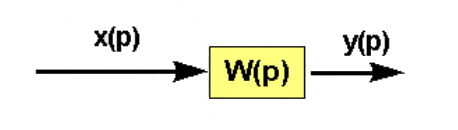
\includegraphics[width=17cm]{transf1.png}\hss}\hfill\null
  	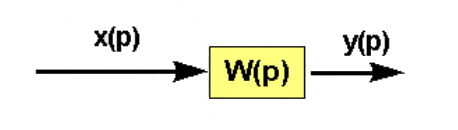
\includegraphics[width=5cm]{transf1.png}
    \caption{Modèle quelconque}
	\end{figure}
	
	Nous aurons donc la fonction de transfert suivante : W(p) = Y(p) / x(p).
	
	\newpage
	
	\chapter{Première manipulation}
	
		\section{Introduction}
	
		À travers cette première manipulation, nous avons cherché à déterminer la fonction de transfert de notre modèle, en visualisant à l'aide d'un graphique, les données fournies en entrée du système (provenant du DAC), ainsi que les données en sortie de notre modèle (une fois traitées par le contrôleur moteur).
		En procédant ainsi, nous allons pouvoir observer et comparer l'évolution de nos courbes en fonction du temps et ainsi déterminer si ces dernières évoluent selon le même schéma, ou si le traitement des données par le contrôleur moteur induit un retard au sein du système.
		
	On retrouve, ci-dessous, le schéma bloc de la première manipulation réalisée.
		
	\begin{figure}[!ht]
    \center
    %\hfill\hbox to 0pt{\hss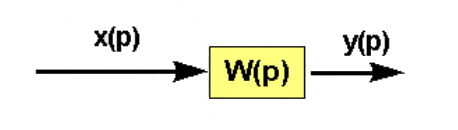
\includegraphics[width=17cm]{transf1.png}\hss}\hfill\null
  	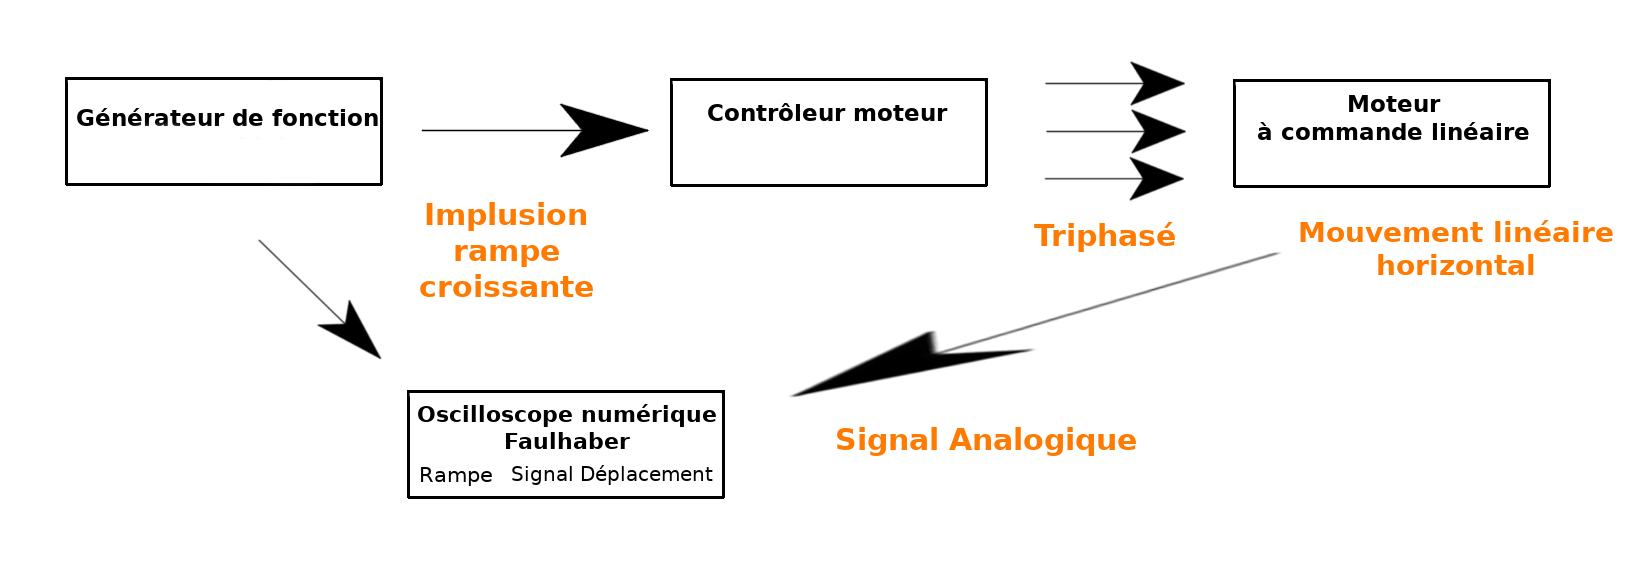
\includegraphics[width=18cm]{manip1.png}
    \caption{Schéma bloc - Première manipulation}
	\end{figure}	
		
		Tel que illustré ci-dessus, nous utilisons un générateur de fonction afin de transmettre une impulsion au contrôleur moteur, sous la forme d'une rampe croissante.
		Grâce à l'oscilloscope numérique intégré au sein du logiciel de configuration des contrôleurs Faulhaber, nous avons pu mesurer la position du barreau aimanté en fonction du temps, via l'exploitation des données provenant des capteurs à effet hall, ainsi que le niveau de tension du signal analogique d'entrée.
		
		De plus, le contrôleur moteur de Faulhaber proposant différents modes de contrôle pour le moteur, tel qu'un contrôle en position, en vitesse et en accélération, nous avons cherché à exploiter les données mesurées, afin de caractériser ces différents modes de contrôle et valider ou non, leur bon fonctionnement, en accord avec le comportement souhaité.
		
		Nous avons, tout d'abord, commencé par tracer sous forme de graphiques, les courbes des trois différents modes de contrôle proposés par le contrôleur sous différents niveaux de tension, variant sur un intervalle allant de 1 volt, jusqu'à 5 volts.
		De plus, nous avons également mesuré, pour chaque niveau de tension, l'évolution de la grandeur analogique en entrée du contrôleur moteur. Tracer les courbes d'évolution des grandeurs analogiques en entrée nous permet de nous assurer que les signaux discrets échantillonnés et utilisés par le contrôleur, correspondent bien aux signaux fournis par le générateur de fonction.
		
		On retrouve ainsi, les graphiques suivants:
		
	\textsc{\begin{figure}[h]
     \begin{minipage}[c]{.46\linewidth}
         \centering
         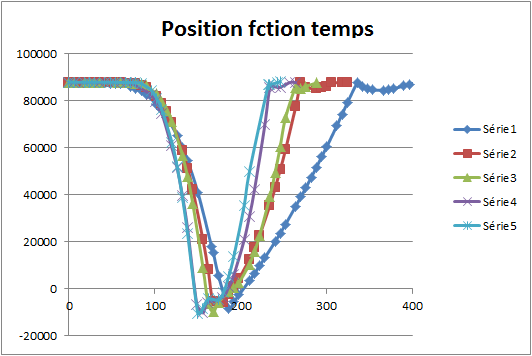
\includegraphics[width=8.3cm]{m1_pos.png}
         \caption{Graphique de position en fonction du temps}
     \end{minipage}
     \hfill%
     \begin{minipage}[c]{.46\linewidth}
         \centering
         \includegraphics[width=9cm]{m1_speed.png}
         \caption{Graphique de vitesse en fonction du temps}
     \end{minipage}
     \hfill%
     \begin{minipage}[c]{.46\linewidth}
         \centering
         \includegraphics[width=8.3cm]{m1_torque.png}
         \caption{Graphique d'accélération en fonction du temps}
     \end{minipage}
     \hfill%
     \begin{minipage}[c]{.46\linewidth}
         \centering
         \includegraphics[width=9cm]{m1_AnIn.png}
         \caption{Graphique des entrées analogiques en fonction du temps}
     \end{minipage}
 	\end{figure}} 
		
	Dans un premier temps, pour chacun des graphiques ci-dessus, on peut observer une évolution des courbes, qui paraît être en accord avec le comportement attendu. Ainsi, que l'on analyse le mode de position, de vitesse, ou d'accélération, on peut observer que l'ensemble des courbes décroissent de plus en plus rapidement, plus le niveau de tension appliqué devient élevé. Il en va de même pour les courbes du graphique de l'entrée analogique en fonction du temps, plus le niveau de tension augmente, plus la pente des rampes devient importante. Ainsi, jusqu'ici, nous restions plutôt confiants.
	
	Par la suite, nous avons commencé à nous intéresser et nous concentrer sur le mode de contrôle en accélération (mode torque) de notre contrôleur. En effet, étant donné qu'à l'aide de notre module, nous captons le signal d'accélération de la touche de notre piano, l'utilisation du contrôle en accélération (torque) de notre contrôleur nous parut comme étant un choix intéressant et logique pour le contrôle des moteurs; nous permettant de travailler sur les données brutes du signal d'accéléromètre, 	sans besoin de l'intégrer pour en obtenir la vitesse et donc d'intégrer avec ce dernier, des erreurs.
	
	Étant donné que les données sont obtenues par intégrations successives, donc par sommes successives, les mesures ne peuvent pas être prises réellement en continu; donc, les sommes introduiront nécessairement de petites erreurs. D'autre part, même avec une mesure parfaitement exacte de l'accélération, on se retrouve avec une estimation de la vitesse qui dérive petit à petit, en fonction des erreurs accumulées. La position est obtenue en intégrant la vitesse, y compris son erreur d'intégration. Ainsi, l'erreur de position sera quadratique par rapport aux approximations initiales. 
	
	C'est pour cette raison, que nous nous sommes appliqués à mettre en place le contrôle en accélération sur notre contrôleur. Mais avant d'implanter cette solution, nous avons tout de même cherché à vérifier si ce dit mode de contrôle en accélération (mode torque), appliquait au moteur un comportement image de l'accélération mesurée. Même si ce mode de contrôle paraissait être "idéal" pour le projet, un premier élément attira notre attention. Ce mode de contrôle en accélération étant nommé contrôle "Torque", il traduirait l'application d'un couple sur notre moteur, pour mettre ce dernier en mouvement, hors un couple appliqué à un moteur en translation, paraît quelque peut contradictoire.
	Une fois la documentation du contrôleur vérifiée, il s'avère que ce mode de contrôle "Torque" soit un asservissement numérique sous la forme d'un correcteur Proportionnel Intégral (PI) en courant; ce dernier combinant l'action des correcteurs précédents pour améliorer les performances globales du système asservi. Mais, bien qu'étant un asservissement en courant, une solution de contrôle, plutôt aisée à mettre en oeuvre, serait de comparer la courbe du contrôle en accélération avec la courbe de la deuxième dérivée du contrôle en position. En procédant ainsi, nous devrions avoir deux courbes ayant la même allure, permettant ainsi de valider le comportement du contrôle en accélération.
	
	\newpage
	
		\section{Caractérisation du mode de contrôle en accélération ou mode "Torque"}

	Souhaitant obtenir une courbe d'accélération en nous basant sur un mode de contrôle en position, il va donc nous falloir dériver deux fois notre fonction, afin d'obtenir une courbe d'accélération exploitable.
	Notre système à dériver étant une fonction discrète, nous allons calculer sa dérivée première comme suivant: 
	
	\[	
		f'(x) = \frac{f(x+h) - f(x-h)}{2h}
	\]
	
	puis, sa dérivée seconde:
	
	\[	
		f''(x) = \frac{f(x+h) - 2f(x) + f(x-h)}{h^2}
	\]
	
	
		\textsc{\begin{figure}[h]
    	\begin{minipage}[c]{.46\linewidth}
         \centering
         \includegraphics[width=8.3cm]{fscd.png}
         \caption{Graphique de la dérivée seconde de la position en fonction du temps}
    	\end{minipage}
     	\hfill%
     	\begin{minipage}[c]{.46\linewidth}
         \centering
         \includegraphics[width=9cm]{torque.png}
         \caption{Graphique de l'accélération en fonction du temps}
    	\end{minipage}
		\end{figure}}
		
		Grâce aux graphiques ci-dessous, nous pouvons nous apercevoir que nos deux graphiques ont une allure en rien comparable, jetant un doute sur le fonctionnement du mode "Torque" de notre contrôleur moteur; posant la question du rôle de ce mode de contrôle, si ce dernier n'est pas destiné à être image d'un contrôle en accélération.
		De plus, outre la non-adéquation avec le mode de contrôle "Torque", nous nous sommes demandés si le traitement du signal analogique par le contrôleur moteur, pouvait ou non, induire un retard, un décalage temporel entre la consigne mesurée et l'établissement de la valeur de contrôle en sortie du contrôleur.
		
		\newpage
		
		\section{Du retard induit}
		
		Suite à la caractérisation du mode "Torque", comme nous l'avons dit précédemment, l'induction d'un retard entre la consigne mesurée et l'établissement de la valeur de contrôle en sortie du contrôleur, si elle existe, peut être un obstacle à l'établissement de notre fonction de transfert.
		
		Pour cela, à l'aide des données relevées plus tôt à partir des capteurs à effet hall, nous avons tracé de nouveaux graphiques afin de pouvoir visualiser le signal de contrôle, ainsi que le signal de consigne appliqué en entrée du contrôleur en fonction du temps.
		
		Nous avons commencé par appliquer un signal carré avec notre générateur de fonction, d'une amplitude variant d'un volt jusqu'à cinq volts; en comparant les différents jeux de mesures réalisées sur la même base de temps, on arrive à un retard moyen d'une valeur de douze millisecondes.
		
		Ensuite, nous avons effectué le même test en appliquant une rampe croissante avec notre générateur de fonction et nous avons pu observer un retard d'en moyenne 10 millisecondes entre la consigne et le signal de sortie.
		
		\section{Conclusion}
		Après avoir cherché à caractériser le comportement du contrôle en accélération de notre contrôleur moteur, puis après avoir observé le retard induit dans notre système par ce même contrôleur moteur, nous pouvons conclure que la manipulation mise en place, ne nous permet pas de pouvoir établir la fonction de transfert de notre module.
		
		Pour cela, nous allons mettre en place une seconde manipulation, dans laquelle le retard n'aura pas d'incidence. De plus, cette manipulation aura aussi l'avantage de nous permettre de mieux caractériser le contrôle "Torque" du contrôleur.
		
		\newpage		
		
	\chapter{Seconde manipulation}
	
		\section{Introduction}
	
		Comme nous avons pu le voir précédemment, lors de la première manipulation, le retard induit par le contrôleur moteur nous a posé soucis dans la première manipulation. Du fait de ce retard, il nous était impossible de mettre en place un modèle afin de pouvoir déduire notre fonction de transfert.
		
		Pour cela, nous avons mis en place cette deuxième expérience, qui a pour but de nous permettre de sortir un modèle, au sein duquel le retard n'aurait pas d'incidence; mais ne serait qu'un élément de l'équation à faire varier pour établir notre modèle. Pour cette manipulation, nous avons procédé, comme l'illustre le schéma bloc ci-dessous.		
		
	\begin{figure}[!ht]
    \center
    %\hfill\hbox to 0pt{\hss\includegraphics[width=17cm]{transf1.png}\hss}\hfill\null
  	\includegraphics[width=18cm]{manip2.png}
    \caption{Schéma bloc - Seconde manipulation}
	\end{figure}	
	
		Nous utilisons encore une fois notre générateur de fonction afin de générer un signal sinusoïdale à destination de notre contrôleur, ce signal analogique sinusoïdale sera varié selon deux paramètres. Tout d'abord son amplitude, évoluant sur un intervalle de trois volts jusqu'à cinq volts, puis c'est la fréquence du signal que nous ferons varier; fréquence qui devra évoluer entre vingt Hertz et 100 Hertz.	Faire varier ces paramètres va nous permettre de vérifier le paramètre ayant une incidence majeure sur le comportement du contrôleur.

	De plus, nous avons placé un accéléromètre sur notre bras aimanté, afin de pouvoir tracer sa courbe de réponse sur l'axe "Z" sur notre oscilloscope. Tracer cette courbe de réponse en même temps que la courbe fournie par le générateur de fonction va nous permettre d'observer l'ensemble des différences entre ces deux courbes et d'en déduire le déphasage ainsi que le retard.
	
	Enfin, nous pourrons également mieux tenter de caractériser notre contrôle en accélération, étant donné que nous pourrons comparer des grandeurs physiques de même nature en entrée, comme en sortie du système. Ces données pourront être analysées au travers d'un diagramme de BODE.
	
		\section{Traitement des données}
		
		Afin de caractériser notre fonction de transfert, nous avons tout d'abord commencé par représenter sous forme de graphique notre nouveau système, afin de pouvoir observer les différences entre les deux courbes obtenues.
		On retrouve, ci-dessous, trois graphiques à titre d'exemple des mesures effectuées; mesures ayant également été prises pour les valeurs de fréquences suivantes : 20Hz, 30Hz, 40Hz, 50Hz, 70Hz et 100Hz. 
		
	\textsc{\begin{figure}[h]
     \begin{minipage}[c]{.46\linewidth}
         \centering
         \includegraphics[width=8.3cm]{osciAcc_3v.png}
         \caption{Graphique oscillo - accéléromètre - 20Hz, 3 Volts}
     \end{minipage}
     \hfill%
     \begin{minipage}[c]{.46\linewidth}
         \centering
         \includegraphics[width=9cm]{osciAcc_4v.png}
         \caption{Graphique oscillo - accéléromètre - 20Hz, 4 Volts}
     \end{minipage}
     \hfill%
     \begin{minipage}[c]{.46\linewidth}
         \centering
        \includegraphics[width=8.3cm]{osciAcc_5v.png}
         \caption{Graphique oscillo - accéléromètre - 20Hz, 5 Volts}
     \end{minipage}
 	\end{figure}}
 	
 	Grâce à nos graphiques ci-dessus, on peut observer que nos deux courbes, image du signal sinusoïdale fournie par le générateur de fonction, ainsi que le signal issu de notre accéléromètre analogique, sont quasiment en opposition de phase (pour un déphasage avoisinant les 180 degrés). Mais pour le moment, il nous est impossible de déterminer si nos courbes sont déphasées ou si le signal analogique de l'accéléromètre est en retard par rapport au signal du générateur de fonction; retard pouvant être dû à notre contrôleur moteur.
 	
 	Afin de déterminer si nous sommes en présence d'un retard, d'un déphasage, ou des deux, nous avons procédé comme suivant.
 	Dans un premier temps, nous avons reconstruit deux signaux sinusoïdaux, en nous basant sur leur équation, afin de pouvoir faire varier leurs paramètres et ainsi en déduire le déphasage et/ou le retard.
 	Le premier signal reconstitué se base sur le signal du générateur de fonction. Dans ce cas-ci, il nous est possible de négliger le retard, étant le signal premier.
	
	\[	
		f(x) = Offset + Ampl * Sin( 2*Pi*F*(T) + Dephasage )
	\]	
	
	Le deuxième est l'image du signal fournie par l'accéléromètre, fonction dans laquelle, nous intégrons cette fois, la notion de retard.
	
	\[	
		f(x) = Offset + Ampl * Sin( 2*Pi*F*(T-retard) + Dephasage )
	\]	
	
	Enfin, nous avons effectué une minimisation sous contrainte sur la fonction sinus, précédemment reconstruite, afin de déterminer les coefficients de déphasage, de retard et d'amplitude, tout en fixant des paramètres tels que l'amplitude et la fréquence. Cette méthode nous a donc permis de déterminer de manière précise, le déphasage entre nos deux courbes, ainsi que les rapports d'amplitudes entre ces dernières, comme nous pouvons l'observer sur la figure ci-dessous:
	
	\begin{figure}[!ht]
    \center
    %\hfill\hbox to 0pt{\hss\includegraphics[width=17cm]{transf1.png}\hss}\hfill\null
  	\includegraphics[width=10cm]{dephAmp.png}
    \caption{Minimisation de la fonction sinus}
	\end{figure}	
	
	Disposant maintenant de l'ensemble des rapports d'amplitudes et de déphasages entre nos signaux analogiques, il nous est possible de tracer la courbe de déphasage en fonction de la fréquence et de l'amplitude en fonction de la fréquence.
	 	
		\begin{figure}[!ht]
    \center
    %\hfill\hbox to 0pt{\hss\includegraphics[width=17cm]{transf1.png}\hss}\hfill\null
  	\includegraphics[width=15cm]{dFctionFreq.png}
    \caption{Déphasage en fonction de la fréquence}
	\end{figure}	
	
	\begin{figure}[!ht]
    \center
    %\hfill\hbox to 0pt{\hss\includegraphics[width=17cm]{transf1.png}\hss}\hfill\null
  	\includegraphics[width=15cm]{AFctionFreq.png}
    \caption{Amplitude en fonction de la fréquence}
	\end{figure}
	
	Grâce aux courbes ci-dessous, on peut observer que nous disposons enfin d'un modèle à partir duquel nous pouvons déterminer une fonction de transfert de notre système. Mais avant cela, il nous reste un dernier graphique à analyser; disposant des rapports d'amplitudes entre nos signaux analogiques, nous pouvons réaliser un diagramme de BODE. Ce diagramme devrait nous permettre de pouvoir caractériser, de manière précise, notre contrôleur moteur.
	
	\begin{figure}[!ht]
    \center
    %\hfill\hbox to 0pt{\hss\includegraphics[width=17cm]{transf1.png}\hss}\hfill\null
  	\includegraphics[width=15cm]{baud.png}
    \caption{Diagramme de BODE}
	\end{figure}	
	
	Comme nous pouvons le voir ci-dessus, notre diagramme de BODE qui devrait être horizontal, s'avère avoir une pente de six db/octave, ce qui traduit que nous sommes déjà dans la pente de la bande rejetée, alors que nous sommes très loin de la valeur de la fréquence de coupure étant de 1 KHz.
	
	\begin{figure}[!ht]
    \center
    %\hfill\hbox to 0pt{\hss\includegraphics[width=17cm]{transf1.png}\hss}\hfill\null
  	\includegraphics[width=15cm]{bode.png}
    \caption{Diagramme générique de BODE}
	\end{figure}
	
\newpage	
	
		\section{Conclusion}
			Après avoir reconstruit des signaux sinusoïdaux, puis effectué une minimisation sous contrainte, afin de pouvoir déterminer les coefficients de déphasage ainsi que les rapports d'amplitudes entre le signal de notre oscilloscope et de notre accéléromètre, nous avons pu réaliser des graphiques nous permettant de déduire une fonction de transfert de notre système.
			
			Mais suite à la modélisation du diagramme de BODE, nous pouvons conclure qu'étant déjà dans la courbe de fréquence rejetée, le contrôle en accélération de notre contrôleur ne paraît pas être viable, invalidant de ce fait nos courbes devant nous permettre de déterminer notre fonction de transfert.
			
\newpage
			
		\chapter{Ouverture}
	
		Etant donné les échecs connus avec les deux précédentes manipulations, une troisième doit être mise en place afin de déterminer efficacement le contrôle en vitesse du contrôleur.
		
		Pour cela, nous allons procéder comme illustré sur le schéma bloc ci-dessous. La manipulation reprend le même principe que la deuxième, à la différence que nous allons intégrer le signal de l'accéléromètre au sein du FPGA pour fournir au contrôleur une courbe en adéquation avec un contrôle en vitesse.
		
	\begin{figure}[!ht]
    \center
    %\hfill\hbox to 0pt{\hss\includegraphics[width=17cm]{transf1.png}\hss}\hfill\null
  	\includegraphics[width=18cm]{manip3.png}
    \caption{Schéma bloc - ouverture manipulation futur}
	\end{figure}
	
	De  plus, le deuxième accéléromètre ne sera pas fixé physiquement sur le deuxième moteur, ce qui va nous permettre de le brancher à divers endroits dans le système afin de pouvoir identifier des sources de déphasage ou de retard. Ainsi, nous pourrons disposer d'une caractérisation très précise de notre système et pouvoir disposer d'une fonction de transfert viable.
	
	
	
	%--------------------------------------------------------------------------------------
%
%	Les cartes réalisées
%		Minimiser la board de l'accéléromètre
%		Ampli AOP et fin de course optique
%		Mezanine du FPGA
%
%--------------------------------------------------------------------------------------
\part{Les circuits imprimés réalisés}
	
	\section{Accéléromètre - evalBoard}
		Alors que nous réalisions la conception de notre chaîne de contrôle, nous avons travaillé avec la carte d'évaluation du constructeur, étant fournie montée avec un accéléromètre, permettant une prise en main rapide du device. Plus tard, après avoir fini la conception de cette chaîne de mesure, il nous a fallu monter notre PCB sur un marteau de la maquette de piano, ce qui a soulevé un "problème" dont nous étions déjà au fait; la carte d'évaluation étant trop grande. Devant s'insérer au sein d'une mécanique de précision, nous avons donc des contraintes de tailles précises à respecter afin d'équiper notre mécanique.
		
		Nous avons donc conçu un nouveau PCB sous l'outil de conception et de routage "KICAD", répondant à nos contraintes de taille; en voici une illustration.
		
 \textsc{\begin{figure}[h]
     \begin{minipage}[c]{.46\linewidth}
         \centering
         \includegraphics[width=7cm]{PCB.PNG}
     \end{minipage}
     \hfill%
     \begin{minipage}[c]{.46\linewidth}
         \centering
         \includegraphics[width=7cm]{3D_print.PNG}
     \end{minipage}
 \end{figure}}
 
 Une fois ce PCB à disposition, il nous a fallu l'insérer au sein de notre maquette. Pour cela, nous avons travaillé avec le service mécanique, second corps de métier travaillant sur le projet, ayant repensé l'ensemble de la mécanique interne du piano, afin de pouvoir insérer divers PCB dans ce dernier.
 
 Le résultat de ce travail en collaboration, fut le support d'accéléromètre si dessous, nous permettant de fixer le PCB précédemment créé, sur le marteau, afin d'offrir une plateforme stable, assurant la bonne qualité des mesures effectuées.
 
 \textsc{\begin{figure}[h]
     \begin{minipage}[c]{.46\linewidth}
         \centering
         \includegraphics[width=7cm]{Accelerometre_v2.JPG}
     \end{minipage}
     \hfill%
     \begin{minipage}[c]{.46\linewidth}
         \centering
         \includegraphics[width=7cm]{montage.jpg}
     \end{minipage}
 \end{figure}}
	
	
	\section{Ampli AOP et intérupteur fin de course}
	
	La conception de cette carte fut motivée par deux éléments. Dans un premier temps, lors de futurs manipulations, nous allons avoir besoin de détecter lorsqu'une touche est au repos ou non, ce qui est rendu possible, grâce à l'utilisation d'interrupteur fin de course "optique" (une photodiode permettant de piloter un transistor). De plus, lors de manipulations sur notre banc de test, nous pensions avoir besoin de pouvoir amplifier un signal analogique provenant d'un générateur de fonction ou d'un capteur quelconque.
	
	C'est pourquoi, nous avons mis au point ce PCB, composé d'un AOP et d'un circuit intégré permettant le contrôle de nos interrupteurs.
	
	\textsc{\begin{figure}[h]
     \begin{minipage}[c]{.46\linewidth}
         \centering
         \includegraphics[width=7cm]{OPB&AOP_1.PNG}
     \end{minipage}
     \hfill%
     \begin{minipage}[c]{.46\linewidth}
         \centering
         \includegraphics[width=7cm]{OPB&AOP_4.PNG}
     \end{minipage}
 \end{figure}}
 
	
	\section{Mezzanine pour connection de meilleur qualité}
	
	La réalisation de cette carte fut, de nombreuses fois, remise à plus tard, étant donné le prototypage rapide mise en place, la maquette a souvent été amenée à évoluer au fur et à mesure de la conception de la chaîne. Mais une fois notre modèle aboutit, ainsi que les problèmes de métastabilité rencontrés, nous nous sommes concentrés à la réalisation de la carte de connexion.
	
	\textsc{\begin{figure}[h]
     \begin{minipage}[c]{.46\linewidth}
         \centering
         \includegraphics[width=7cm]{3D_TOP.PNG}
     \end{minipage}
     \hfill%
     \begin{minipage}[c]{.46\linewidth}
         \centering
         \includegraphics[width=7cm]{3D_BOTTOM.PNG}
     \end{minipage}
 \end{figure}}
	
		
%--------------------------------------------------------------------------------------
%
%	Elément de fin de document
%		Conclusion
%		Bibliographie
%		Table des figures
%
%--------------------------------------------------------------------------------------

\part{Conclusion}

	Clôturant mes cinq années d'études à l'UTBM (Université de Technologie de Belfort-Montbéliard), j'ai effectué mon stage de fin d'étude au laboratoire de Physique Nucléaire et des Hautes Energies de Paris, au sein du service électronique, sous la tutelle de Monsieur Hervé LEBBOLO.

Le projet mené vise la réalisation d'un système de motorisation asservie de la mécanique d'un piano à queue afin d'offrir de nouvelles couleurs aux préparateurs de pianos, ainsi que de nouvelles voies d'expression musicales aux interprètes tout en gardant intact le toucher traditionnel des mécaniques à répétition.

Ce stage fut, pour moi, une véritable chance, me permettant de lier ma passion de la musique à mon domaine d'étude, de plus, il fut pour moi l'occasion de découvrir de nouvelles technologies liées au monde du système embarqué, de parfaire mes connaissances en traitement du signal, ainsi que d'être formé à la conception, au routage et à la fabrication de PCB.

Au travers du développement de notre chaîne de contrôle, j'ai pu appréhender de nouvelles technologies, qui m'étaient inconnues, le développement sur processeur FPGA, soutenu par le langage VHDL. De plus, au travers des manipulations sur banc de test, j'ai pu parfaire mes compétences en traitement du signal, afin de proposer une fonction de transfert pour notre système. Enfin, la conception de PCB sous KICAD fut pour moi l'occasion d'être formé à un aspect de mon métier plus orienté électronique.

De plus, de part l'autonomie de travail qui me fut accordée, j'ai eu à ma charge la gestion de mon temps, ainsi que la gestion de mon projet, sans contrainte. Cette expérience aura été pour moi l'occasion d'appréhender la gestion d'un projet de grande envergure, impliquant des personnes travaillant dans divers services et donc de diverses compétences.


\part{Bibliographie}

	\begin{itemize}
		\item Descriptif global du projet: BHLS-CNRS-UPMC-LPNHE-IRCAM.pdf
		\item Module opensource SPI VHDL - https://eewiki.net/pages/viewpage.action?pageId=4096096
		\item Introduction au VHDL:
						- https://sti.discip.ac-caen.fr/IMG/pdf/vhdl.pdf
						- http://www.montefiore.ulg.ac.be/\~senny/download/ELEN040\_TranspVHDL.pdf
						- http://lslwww.epfl.ch/pages/teaching/cours\_lsl/sl\_info/19.VHDL.pdf
						- http://hdl.telecom-paristech.fr/vhdl\_intro.html
						- https://tcuvelier.developpez.com/tutoriels/vhdl/introduction-langage/
						- http://perso.citi.insa-lyon.fr/trisset/cours/MAC-TC/cours-VHDL.pdf
		\item FIFO en VHDL - https://vlsicoding.blogspot.com/2013/10/design-synchronous-fifo-in-vhdl.html
		\item Buffer circulaire en VHDL - http://www.ece.ualberta.ca/\~elliott/ee552/studentAppNotes/1999f/circular\_buffer/circular\_buffer.html
		\item VHDL norme 2008 - https://www.doulos.com/knowhow/vhdl\_designers\_guide/vhdl\_2008/vhdl\_200x\_ease/
		\item ModelSim manual Reference - https://users.ece.cmu.edu/\~kbiswas/se\_cmds.pdf
	\end{itemize}


\part{Table des figures}

	\listoffigures
	
\part{Annexe}

	\chapter{Conception PCB - accéléromètre evalBoard}
		\includepdf[scale=1, pages=-]{FICHE_FABRICATION_OPBANDAOP.pdf}
		\includepdf[scale=1, pages=1]{FICHE_LIAISON_SCHEMA_PCB_NEWS.pdf}	
		\includepdf[scale=1, pages=1]{FICHIER_DIMENSION_EVALBOARD.pdf}
		\includepdf[scale=1, pages=-]{PLAN_CABLAGE_TOP_ELEMENTS_EVALBOARD.pdf}
		\includepdf[scale=1, pages=-]{PLAN_PERCAGE_EVALBOARD.pdf}
		\includepdf[scale=1, pages=-]{EVAL_Printing_Impression_Schematique.pdf}	
		\hfill\hbox to 0pt{\hss\includegraphics[width=15cm]{Liste_compos.png}\hss}\hfill\null\newline
			
	\chapter{Conception PCB - Ampli AOP et intérupteur fin de course}
		\includepdf[scale=1, pages=-]{AOP_FICHE_FABRICATION_OPBANDAOP}
		\includepdf[scale=1, pages=-]{AOP_FICHE_LIAISON_OPBANDAOP}	
		\includepdf[scale=1, pages=-]{AOP_FICHIER_DIMENSION_OPBANDAOP}
		\includepdf[scale=1, pages=-]{AOP_PLAN_CABLAGE_BOTTOM_ELEMENTS_OPBANDAOP}
		\includepdf[scale=1, pages=-]{AOP_PLAN_CABLAGE_TOP_ELEMENTS_OPBANDAOP}
		\includepdf[scale=1, pages=-]{AOP_PRINTING_IMPRESS_SCHEMATIC}	
		\includepdf[scale=1, pages=-]{AOP_PLAN_PERCAGE_OPBANDAOP}		
		
		\hfill\hbox to 0pt{\hss\includegraphics[width=15cm]{AOP_Liste_Compos.png}\hss}\hfill\null\newline
		
		\hfill\hbox to 0pt{\hss\includegraphics[width=15cm]{AOP_ListeComposants.png}\hss}\hfill\null\newline
		
	\chapter{Conception PCB - Mezzanine}
		\includepdf[scale=1, pages=-]{M_FICHE_FABRICATION_MEZZA}
		\includepdf[scale=1, pages=-]{M_FICHE_LIAISON_MEZZA}	
		\includepdf[scale=1, pages=-]{PLAN_CABLAGE_BOTTOM_ELEMENTS_MEZZA}
		\includepdf[scale=1, pages=-]{PLAN_CABLAGE_TOP_ELEMENTS_MEZZA}
		\includepdf[scale=1, pages=-]{PLAN_PERCAGE_MEZZA}
		\includepdf[scale=1, pages=-]{M_PRINTING_IMPRESS_SCHEMATIC}	
		
	\chapter{Projet - Présentation par Faulhaber}
		\includepdf[scale=1, pages=-]{dff_180285_motion_1_2018_fr_fin.pdf}

\end{document}

